\documentclass[11pt]{article}
\usepackage[margin=1in]{geometry}
\usepackage{amsmath,amssymb,amsthm}
\usepackage{graphicx}
\usepackage{booktabs}
\usepackage{array}
\usepackage[colorlinks=true,linkcolor=blue,citecolor=blue,urlcolor=blue]{hyperref}
\usepackage{natbib}
\emergencystretch=3em
\newtheorem{prop}{Proposition}

\title{The Mass-Tracking Closure in Four-Dimensional Quasi-Topological Gravity:\\
Double-Null Equations, an Exact Generalized-Mass Law\\
and Evolution from Event-Horizon-Regular Data}
\author{Gracen Ownby}
\date{}

\begin{document}
\maketitle

\begin{abstract}
The series' regular black hole is the Hayward metric, whose static sector is realized in four-dimensional quasi-topological gravity with $h(\psi)=\psi/(1-\ell^{2}\psi)$. We write the field equations with a massless scalar field in double-null form, derive them from the reduced action, and obtain an exact law for the generalized mass, $\partial_vm=8\pi r^{2}y\phi_v^{2}$, for every $h$. For data regular on the event horizon $y\ge\tfrac12$, so $m$ cannot decrease; the finite-time singularity of interior characteristic data belongs to the branch $y<0$. A constrained evolution from such data agrees with an independent fourth-order code to $10^{-7}$ in $r$. For tail amplitudes $3\times10^{-4}$--$3\times10^{-2}$ the interior flux is the linear kernel of Paper~G, the metric exponent is $-\kappa_-(m_f)$, and a front arrives behind which $\psi\to1/\ell^{2}$, $m$ grows linearly and the Kretschmann invariant exceeds $10^{25}\ell^{-4}$: the curvature bound of the static solutions does not extend to the dynamical interior. The accurate range of a scheme of order $p$ is limited by an error growing as $h_v^{p}e^{\kappa_+v}$, explained by a one-dimensional model with one fitted constant; evolving the difference from the exact horizon solution removes it (regular to $\kappa_+v\simeq69$). Behind the front the solution is slaved to the interior flux, and $K\propto v^{4k-2}$ for a tail $v^{-k}$ is an extrapolation supported over the simulated range. A collapse of a compact scalar pulse generates the tail $v^{-3}$; for strong pulses its coefficient is $F\cdot8m_f|Q|$ with $F=1-Q_{\rm abs}/Q_0$ ($Q_0$ the Noether charge of the data, $Q_{\rm abs}$ the charge absorbed by the growing event horizon), to $0.05\%$ on average in $22$ cases. The identification of $Q_{\rm abs}$ with the horizon term of the time-inverted Newman--Penrose constant of Gajic and Kehrberger is conditional: the hypotheses of their theorem (a given metric settling to Schwarzschild) were not verified for the collapse data, and of that paper the statements of Sections~1--4, the derivation of the $\ell=0$ constant (Proposition~7.1, Lemma~7.2), Sections~6, 8, 9 and the appendices were read, the energy estimates of Section~5 and the iteration of Sections~7.4--7.8 were not; for a Schwarzschild exterior the coefficient $8M|Q|$ is also obtained here independently, to first order in $M$ and by a numerical evolution ($1.000$ to $10^{-3}$). Not established: extendibility at $v=\infty$ and timelike tidal forces.
\end{abstract}

\section{Introduction}
\label{sec:intro}

The preceding papers of this series use the Hayward metric~\citep{Hayward2006}
\begin{equation}
f(r)=1-\frac{2mr^{2}}{r^{3}+2m\ell^{2}}
\label{eq:hayward}
\end{equation}
with a length $\ell$ fixed and a mass parameter $m$ that tracks the mass of the hole (the closure $s=0$ of Paper~E~\citep{PaperE}). Paper~E asked whether the inner horizon of this metric survives perturbation. It answered with a thin-shell model that holds for any closure $M(m,r)$ and with a nonlinear double-null evolution that holds only for the \emph{additive} closure $M=\mu+M_N(r)$, because the Einstein--nonlinear-electrodynamics system has no closure in which the mass parameter tracks the Misner--Sharp mass. Paper~G~\citep{PaperG} developed a late-time method for that additive system: data regular on the event horizon, the linear response of the static interior to the horizon flux, and exact integration of the mass along a ray. The open point is therefore the following: the series' metric is the static solution of a theory, if one exists, whose field equations couple $m$ to the dynamics, and until that theory is specified one cannot evolve the interior of~\eqref{eq:hayward}.

Such a theory now exists for the static sector. \citet{BuenoCanoHennigar2024} showed that quasi-topological gravities in dimensions $D\ge5$ admit regular black holes whose metric function is fixed by a single function $h(\psi)$ of the curvature invariant $\psi=(1-f)/r^{2}$; such polynomial theories do not exist in four dimensions, where non-polynomial quasi-topological gravities with the same structure were constructed by \citet{BuenoCanoHennigarMurcia2025}, and \citet{BorissovaCarballoRubio2026} identified the choice $h=\psi/(1-\ell^{2}\psi)$ with the Hayward metric (their Eq.~(156) solves their Eq.~(152), $h=2M/r^{3}$, with this $h$; this choice has a $\psi^{2}$ term and is not generated by the series of \citealt{BuenoCanoHennigarMurcia2025}). The formation of regular black holes by the collapse of thin dust shells in higher-dimensional ($D\ge5$) quasi-topological gravity was studied by \citet{BuenoCanoHennigarMurcia2024}, and the time-dependent spherically symmetric field equations with matter for the non-polynomial four-dimensional theories were obtained by \citet{BuenoCanoHennigarMurcia2025}. \citet{FrolovZelnikov2026} (null-shell collisions in regular black holes of quasi-topological gravity: large amplification only for collisions extremely close to the inner horizon) and \citet{DiFilippo2026} (mass inflation and thin shells in quasi-topological gravity) studied shells and mass inflation in these theories; the latter argue that in standard distributional theory null thin shells are not available for the pure-gravity regular black hole solutions in the standard distributional theory (a conclusion drawn within that theory and, as far as we read, at the level of the abstract of that paper; Ref.~\cite{FrolovZelnikov2026} uses null shells with the Dray--'t~Hooft--Barrab\`es--Israel junction conditions), so that the Ori thin-shell construction of Paper~E need not carry over. This paper uses the first group of results to evolve the interior and compares with the second.

\paragraph{Related work.} Mass inflation at the inner horizon of charged black holes was identified by \citet{PoissonIsrael1989,PoissonIsrael1990} and given an exact model by \citet{Ori1991}; double-null evolutions of scalar-field collapse to charged black holes \citep{BradySmith1995,Burko1997,HodPiran1998}, the late-time analysis of the shock at the inner horizon \citep{MarolfOri2012} and the mathematical theory \citep{Dafermos2005} describe a weak null singularity. For regular black holes in general relativity with matter, \citet{CarballoRubio2022a} construct regular black holes whose inner horizon has vanishing surface gravity (a degenerate inner horizon) and find no exponential mass inflation in the two perturbation models they study, \citet{BonannoPanassitiSaueressig2025} find power-law growth of the Hayward mass function, map its basin of attraction, and find logarithmic growth in an asymptotically safe collapse model, \citet{Iofa2022} computes the flux (in his abstract, the energy density) of scalar perturbations measured by a free-falling observer near the inner horizon of the Hayward black hole, which diverges exponentially there and which he states is not directly connected with mass inflation (the inner mass function itself stays finite in his calculation), and \citet{ShaoGuoTianZhang2025} evolve a scalar field in the Hayward geometry sourced by non-linear electrodynamics and find that a strong field shrinks the inner horizon to zero. In quasi-topological gravity the static vacuum solutions satisfy a limiting-curvature property \citep{BuenoHennigarMurciaVicenteCano2026}, minimally coupled matter breaks the mass-independent bound but sufficient conditions on the stress tensor keep the curvature bounded for static matter \citep{BuenoHennigarMurciaVicenteCano2026}, null-shell collisions give large amplification only extremely close to the inner horizon \citep{FrolovZelnikov2026}, and thin shells are constrained differently from the Ori model \citep{DiFilippo2026}. We are not aware of a double-null evolution, in the quasi-topological theory itself, of a continuous scalar flux from event-horizon-regular data through the inner-horizon region; the present paper is that evolution and reports what it shows about the generalized mass, the metric exponent and the curvature.

\paragraph{What is done.} (1) We write the field equations of Ref.~\cite{BuenoCanoHennigarMurcia2025} for a massless minimally coupled scalar field in double-null form (Section~\ref{sec:eqs}) and verify them by five independent checks that do not rely on the derivation (Section~\ref{sec:checks}). (2) We derive an exact law for the generalized mass along an ingoing ray, $\partial_vm=8\pi r^{2}y\phi_v^{2}$ (Section~\ref{sec:ray}), and prove that data regular on the event horizon have $y\ge\tfrac12$, so that the generalized mass cannot decrease (Section~\ref{sec:prop}). With the range of $h$ the law classifies where $\psi$ can go (Section~\ref{sec:classes}). (3) We report what characteristic data on interior rays do in this system, a finite-advanced-time singularity of the data ray, and explain with the proposition that it belongs to the branch $y<0$, which event-horizon-regular data exclude (Appendix~\ref{sec:num}). (4) We construct event-horizon-regular data for an arbitrary $h$ (Section~\ref{sec:ehdata}) and a constrained evolution that is stable where the free evolution of Paper~E is not (Section~\ref{sec:cy}). (5) We report the evolution of the Hayward $h$ from these data: the interior flux against the linear kernel, the metric exponent, the front of the inflating mass, the state behind it and the curvature (Section~\ref{sec:hay}); and of a bounded $h$ (Section~\ref{sec:model2}). (6) We identify the numerical limit of the run, a growth of the truncation error as $h_v^{p}e^{\kappa_+v}$ ($p$ the order of the scheme; for the second-order code $\propto(B\,h_v)^{2}$), and remove it by refining the advanced-time step alone (Section~\ref{sec:cy}); we show that the state behind the front is slaved to the interior flux and read the endpoint from that structure, with its asymptotics, for three tail exponents (Sections~\ref{sec:slave} and~\ref{sec:endpoint}); (7) we repeat the evolution with a second, independent code of fourth order, which agrees with the first and allows the curvature invariant to be followed to $v\simeq380$, and study that invariant and the tidal integrals along the ingoing null ray in that range (Sections~\ref{sec:code2} and~\ref{sec:curv2}); (8) we derive the mechanism of the limit, remove it by evolving the differences from the exact horizon solution, locate and remove a rounding-level seed of the remaining late-time growth (a step in the initial row), and follow the solution to $\kappa_+v\simeq50$--$69$ for five tail exponents, three amplitudes and three inner masses (Sections~\ref{sec:mech}, \ref{sec:seed} and~\ref{sec:curv3}); (9) we replace the prescribed horizon tail by the one generated by a collapse (a nonlinear double-null stage and a linear stage on the static exterior, with their validation), measure its exponent and amplitude in the Hayward and Einstein cases, drive code~E with it, and repeat the construction with collapse data of nonzero Newman--Penrose constant, which gives the exponent $k=2$ and a coefficient fixed by the data (Section~\ref{sec:collapse}); (10) we scan the strength of a pulse imposed on the horizon and then produce strong pulses by collapse into an existing hole ($m_f/m_0$ up to $5$), which fixes the inner radius at $r_-(m_f)$ and shows that the $v^{-3}$ coefficient is reduced by a factor $F=0.37$--$1$ with respect to the linear identity $B=8m|Q|$; (11) we explain $F$ as one minus the fraction of the Noether charge of the data that the growing event horizon absorbs, verify this in $22$ cases to $0.05\%$ on average ($0.09\%$ at most; the reading of that fraction as the horizon term of a published theorem is conditional, Section~\ref{sec:collapse}), and give a priori estimates of that fraction; (12) we repeat the construction for data with a nonzero scalar charge at infinity (Section~\ref{sec:collapse}).

\paragraph{What is not done.} The field equations are those of the reduced action of Refs.~\cite{BuenoCanoHennigarMurcia2025,BorissovaCarballoRubio2026}; we check that the covariant densities lift that action (Section~\ref{sec:checks}(g)) and that the double-null equations are its Euler--Lagrange equations (Section~\ref{sec:checks}(f)), but we take the four-dimensional theory itself, and the Hayward function as its resummation, from those references; for $\ell^{2}\psi\ge1$ and for $\psi\to-\infty$ the time-dependent equations are an analytic continuation that we adopt and do not prove (the event-horizon-regular solutions of Sections~\ref{sec:hay}--\ref{sec:model2} stay in $0<\psi<1/\ell^{2}$, inside the radius of convergence of the series). We do not include the Hawking flux, we do not simulate beyond $v\simeq1400$ ($\kappa_+v\simeq69$ for $m/\ell=5$; the endpoint is read from a structure verified to that range), we do not classify the singularity at $v=\infty$ (extendibility, tidal forces on timelike observers), and nothing here concerns the Ori shell (Ref.~\cite{DiFilippo2026} argues that null thin shells are not available in standard distributional theory for these theories; Ref.~\cite{FrolovZelnikov2026} uses them with junction conditions). Section~\ref{sec:open} lists what is and is not established.

\section{The theory and the closure}
\label{sec:theory}

In a four-dimensional quasi-topological gravity (Refs.~\cite{BuenoCanoHennigarMurcia2025,BorissovaCarballoRubio2026}; Ref.~\cite{BuenoCanoHennigar2024} for the higher-dimensional polynomial theories with the same structure) the static spherically symmetric solutions are $ds^{2}=-N^{2}f\,dt^{2}+dr^{2}/f+r^{2}d\Omega^{2}$ with $N$ constant and $f$ determined by
\begin{equation}
h(\psi)=\frac{2m}{r^{3}},\qquad \psi\equiv\frac{1-f}{r^{2}},
\label{eq:hpsi}
\end{equation}
where $m$ is an integration constant (the \emph{generalized mass}) and $h$ is the characteristic function of the theory; Einstein gravity is $h=\psi$, for which $f=1-2m/r$. The Hayward metric~\eqref{eq:hayward} is the solution of~\eqref{eq:hpsi} for
\begin{equation}
h(\psi)=\frac{\psi}{1-\ell^{2}\psi},\qquad h'(\psi)=\frac{1}{(1-\ell^{2}\psi)^{2}},
\label{eq:hH}
\end{equation}
because $1-\ell^{2}\psi=r^{3}/(r^{3}+2m\ell^{2})$ for~\eqref{eq:hayward}. Two facts about this realization matter for what follows. First, the Misner--Sharp mass is $M=r^{3}\psi/2=mr^{3}/(r^{3}+2m\ell^{2})$, which is bounded by $r^{3}/2\ell^{2}$ for any $m$, whereas the generalized mass $m$ is not; the mass-tracking closure of Paper~E~\citep{PaperE} is the statement that $m$ is the quantity which is conserved in the vacuum and changed by the flux of matter, the Misner--Sharp mass being a derived function of $(m,r)$. Second, in the quasi-topological theory the field equations determine how $m$ changes (Eq.~\eqref{eq:mlaw} below), so no closure has to be postulated; the additive closure of Paper~E was needed because the Einstein--NED system does not supply one.

For the bounded model of Ref.~\cite{BuenoCanoHennigarMurcia2025} (Eq.~(51) there; ``bounded'' refers to the range of $\psi$, while $h$ itself diverges at $|\psi|=1/\alpha$)
\begin{equation}
h(\psi)=\frac{\psi}{\sqrt{1-\alpha^{2}\psi^{2}}},\qquad h'(\psi)=\frac{1}{(1-\alpha^{2}\psi^{2})^{3/2}},
\label{eq:hB}
\end{equation}
$\psi$ is confined to $(-1/\alpha,1/\alpha)$ in the static solutions and the generalized mass is unrestricted. We call this model~2 and the Hayward model~1; model~0 is Einstein gravity. The static interior of model~1 with $m=5$, $\ell=1$ has $r_-=1.057475$, $r_+=9.897927$, $\kappa_-=0.795649$ (the background of Paper~E at $\mu=0$), and that of model~2 with $m=1$, $\alpha=1$ has $\psi(r_-)=0.8376$; the choice $m=1$ keeps $\psi(r_-)$ away from the wall (interior-data runs, Appendix~\ref{sec:num}). The event-horizon-regular runs of Section~\ref{sec:model2} use $m=1.5$.

\paragraph{Static relations.} From~\eqref{eq:hpsi}, $\psi'(r)=-3h/(rh')$ and so
\begin{equation}
f'(r)=-2r\psi-r^{2}\psi'=rQ(\psi),\qquad Q(\psi)\equiv\frac{3h}{h'}-2\psi .
\label{eq:Q}
\end{equation}
At a horizon $\psi=1/r_h^{2}$ and $\kappa_h=|f'|/2=r_h|Q(\psi_h)|/2$. For Hayward $Q=\psi(1-3\ell^{2}\psi)$, which gives $Q(1/r_-^{2})=-1.5048$ and $\kappa_-=0.7956$ at $r_-=1.0575$, as it must; for $h=\psi$, $Q=\psi$. The sign of $Q'$ at the inner horizon is opposite to that in Einstein gravity ($Q'=1-6\ell^{2}\psi_-=-4.36$ for Hayward); we use $Q$ only through~\eqref{eq:Q} and~\eqref{eq:psiv} below.

\section{Double-null form of the field equations}
\label{sec:eqs}

Take $ds^{2}=-W\,du\,dv+r^{2}d\Omega^{2}$, $W=e^{\sigma}$, a massless scalar $\phi(u,v)$ minimally coupled with the usual stress tensor $T_{\mu\nu}=\partial_\mu\phi\,\partial_\nu\phi-\tfrac12 g_{\mu\nu}(\partial\phi)^{2}$, and
\begin{equation}
\psi=\frac{1}{r^{2}}\Bigl(1+\frac{4r_ur_v}{W}\Bigr),\qquad Q=\frac{3h}{h'}-2\psi,\quad c_1=\frac1{h'},\quad c_2=\frac{9\,h^{2}h''}{4\,h'^{3}},\quad c_3=\frac{h''}{h'^{3}} .
\end{equation}
In the gauge $\varphi=r$ the time-dependent equations of Ref.~\cite{BuenoCanoHennigarMurcia2025} read
\begin{equation}
\partial_r\!\bigl[r^{3}h(\psi)\bigr]=\frac{8\pi G}{N^{2}f}\,r^{2}T_{tt},\qquad
\partial_tf=-\frac{8\pi G}{h'(\psi)}\,rf\,T_{tr},\qquad
\partial_rN=\frac{4\pi G}{h'(\psi)}\,rN\Bigl(T_{rr}+\frac{T_{tt}}{N^{2}f^{2}}\Bigr)
\end{equation}
(Eqs.~(36)--(38) there; $T_{tt}$, $T_{tr}$, $T_{rr}$ are the components of the stress tensor of the scalar). Since $f=(\nabla r)^{2}$ and $\psi=(1-f)/r^{2}$ are scalars, the gauge $\varphi=r$ can be chosen wherever $\nabla r\neq0$, and the first and third equations, rewritten in null coordinates with $T_{uu}=\phi_u^{2}$, $T_{vv}=\phi_v^{2}$ and $T_{uv}=0$, give the two Raychaudhuri-type equations; the combination that defines the static solution, $f'=rQ(\psi)$, gives $r_{uv}$. The remaining equation, for $\sigma_{uv}$, is not independent: it is fixed by the compatibility of the others (Section~\ref{sec:checks}(e)). With $G=1$, then,
\begin{align}
r_{uu}-\sigma_ur_u&=-\frac{4\pi r}{h'}\,\phi_u^{2}, & r_{vv}-\sigma_vr_v&=-\frac{4\pi r}{h'}\,\phi_v^{2},\label{eq:ray}\\
r_{uv}&=-\frac{Wr}{4}\,Q(\psi),\label{eq:ruv}\\
\sigma_{uv}&=\frac{W\psi}{2}-W c_2-\frac{8\pi}{h'}\phi_u\phi_v+\frac{64\pi^{2}c_3}{W}\phi_u^{2}\phi_v^{2},\label{eq:suv}\\
\phi_{uv}&=-\frac{r_u\phi_v+r_v\phi_u}{r}.\label{eq:phi}
\end{align}
For $h=\psi$ ($h'=1$, $h''=0$, $c_2=c_3=0$, $Q=\psi$) these are the Einstein--scalar equations in the form used in Paper~E~\citep{PaperE}: $r_{uv}=-\tfrac14 W r\psi=-\tfrac14(W r^{-1}+4r_ur_v/r)$, $\sigma_{uv}=\tfrac12W\psi-8\pi\phi_u\phi_v$. For a static solution $r_{uv}=ff'/4$ and $\sigma_{uv}=ff''/4$ (interior $f<0$, $W=|f|$), which~\eqref{eq:ruv} and~\eqref{eq:suv} must reproduce from~\eqref{eq:hpsi} (check (b) below).

\paragraph{Status of the equations.} Equations~\eqref{eq:ray}, \eqref{eq:ruv} and \eqref{eq:phi} are our transcription of Ref.~\cite{BuenoCanoHennigarMurcia2025} into null coordinates, and Eq.~\eqref{eq:suv} follows from them by compatibility; we did not find them in this form in the literature. Check~(f) below derives all of them, including the $c_3$ term, from the spherically reduced action of Refs.~\cite{BuenoCanoHennigarMurcia2025,BorissovaCarballoRubio2026}, independently of the transcription. The checks of Section~\ref{sec:checks} test the transcription (not the field equations of the theory). The equations of Ref.~\cite{BuenoCanoHennigarMurcia2025} are proved there for the class of $h$ generated by the theory, which contains the bounded model~\eqref{eq:hB}; the Hayward $h$, which has a $\psi^{2}$ term, is realized by the action of Ref.~\cite{BorissovaCarballoRubio2026}, whose characteristic function is arbitrary and whose spherical reduction has the same Horndeski form (check~(f)).

\section{Checks on the equations}
\label{sec:checks}

The checks (a)--(e) below do not use the equations being tested to produce the reference; (f) derives them from the reduced action and (g) connects that action to the four-dimensional invariants.

(a) \emph{Einstein limit.} The code with $h=\psi$ (model~0) and the code of Paper~E~\citep{PaperE} for the additive closure at $m_N=0$ differ by $9.7\times10^{-17}$ (maximum over the grid, field scale $3.4$) on identical data (\texttt{check\_gr\_limit.py}).

(b) \emph{Static interior.} For the Hayward $h$ with $m=5$ and for the bounded $h$ with $m=1$, equations~\eqref{eq:ruv}--\eqref{eq:suv} reproduce $ff'/4$ and $ff''/4$ computed by finite differences of the exact $f$ to $1.3\times10^{-7}$ and $1.1\times10^{-6}$ (relative, nine radii between $1.05r_-$ and $0.97r_+$; limited by the finite difference) (\texttt{check\_static\_identity.py}).

(c) \emph{Integrability.} The $u$- and $v$-Raychaudhuri equations~\eqref{eq:ray} are compatible with the $r_{uv}$ equation~\eqref{eq:ruv} only if, with $c=4\pi/h'$ and $Q=3h/h'-2\psi$,
\begin{equation}
c\,Q'-c=c'\,(Q+2\psi) .
\label{eq:integrab}
\end{equation}
This is an identity in $h$; we verified it with numerical derivatives of $h$ at six values of $\psi$ for the Hayward $h$ (maximum relative violation $1.8\times10^{-11}$) and five for the bounded $h$ ($2.1\times10^{-9}$). Using $c'=-4\pi h''/h'^{2}$, $Q'=3-3hh''/h'^{2}-2$ and $Q+2\psi=3h/h'$, both sides equal $4\pi\bigl(1-3hh''/h'^{2}\bigr)/h'$ identically, so~\eqref{eq:integrab} is exact for every $h$.

(d) \emph{Convergence of the constraints.} The evolution uses~\eqref{eq:ruv}--\eqref{eq:phi} only, not~\eqref{eq:ray}. The residuals $r_{uu}-\sigma_ur_u+4\pi r\phi_u^{2}/h'$ and the $v$ analog, computed afterwards, converge at second order in the mesh width for both models (rows: model and window in $v$; $A=0.02$, $B=0.002$; entries: relative $L_2$ residual in the $u$ and $v$ directions; \texttt{run\_qtg\_validate.py}, \texttt{validate\_model1.log}, \texttt{validate\_model2.log}). A wrong $\sigma_{uv}$ or $r_{uv}$ would leave an $O(1)$ residual.

\begin{center}\small
\begin{tabular}{lcccc}
\toprule
model, window & $h=0.08$ ($u$, $v$) & $h=0.04$ & $h=0.02$ & orders ($u$; $v$)\\\midrule
1, $v\in[0,20]$ & $4.0\!\times\!10^{-3}$, $3.0\!\times\!10^{-3}$ & $9.9\!\times\!10^{-4}$, $7.5\!\times\!10^{-4}$ & $2.5\!\times\!10^{-4}$, $1.9\!\times\!10^{-4}$ & $2.0$; $2.0$\\
1, $v\in[20,55.2]$ & $5.9\!\times\!10^{-1}$, $6.8\!\times\!10^{-4}$ & $1.4\!\times\!10^{-1}$, $1.7\!\times\!10^{-4}$ & $3.4\!\times\!10^{-2}$, $4.2\!\times\!10^{-5}$ & $2.0$; $2.0$\\
2, $v\in[0,20]$ & $1.2\!\times\!10^{-3}$, $6.1\!\times\!10^{-4}$ & $2.9\!\times\!10^{-4}$, $1.6\!\times\!10^{-4}$ & $7.4\!\times\!10^{-5}$, $4.1\!\times\!10^{-5}$ & $2.0$; $1.9$\\
2, $v\in[20,60]$ & $2.4\!\times\!10^{-2}$, $2.7\!\times\!10^{-4}$ & $5.9\!\times\!10^{-3}$, $6.8\!\times\!10^{-5}$ & $1.5\!\times\!10^{-3}$, $1.7\!\times\!10^{-5}$ & $2.0$; $2.0$\\\bottomrule
\end{tabular}
\end{center}
The static background itself converges at second order (maximum relative error in $r$: $9.3\times10^{-4},\,2.3\times10^{-4},\,5.8\times10^{-5},\,1.5\times10^{-5}$ for $h=0.08,\ldots,0.01$, model~1).

The $u$-residual of model~1 in the second window is large at the coarsest mesh ($0.59$) and falls at second order ($0.14$, $0.034$); we attribute the size to the exponentially small $r_u$ in that window (the residual is relative to $\|r_{uu}\|$) but have not separated that from truncation error in $\sigma_u$. The scheme, like that of Paper~E, loses accuracy as $v$ approaches the singular time of Appendix~\ref{sec:num}.

(e) \emph{Compatibility.} Given~\eqref{eq:ray}, \eqref{eq:ruv} and~\eqref{eq:phi}, the mixed derivative of the Raychaudhuri equation must agree with the $u$-derivative of~\eqref{eq:ruv}, $\partial_v(r_{uu})=\partial_u(r_{uv})$. This is linear in $\sigma_{uv}$ and determines it from the other equations at any point where $r_u\ne0$ (the derivatives of all the fields that appear follow from the equations themselves). We solved it at $2000$ random points (random $r,r_u,r_v,\sigma,\sigma_u,\sigma_v,\phi_u,\phi_v$ with $\psi$ in the domain of $h$) for the Hayward $h$ and the bounded $h$ and compared with~\eqref{eq:suv}, including the coefficient $9/4$ of $c_2$: the maximum relative difference is $3.4\times10^{-12}$ and $3.3\times10^{-10}$ (\texttt{check\_compat.py}). So~\eqref{eq:suv} is not an independent assumption: it is what makes the system consistent, for every $h$ (the integrability identity~\eqref{eq:integrab} is the same statement for the coefficient of $\phi_u^{2}$).

(f) \emph{Derivation from the reduced action.} The tests (a)--(e) check the transcription and its consistency; they do not show that the equations are those of the theory. We therefore derived them from an action. Ref.~\cite{BuenoCanoHennigarMurcia2025} (Eqs.~(22)--(26) there) reduces the four-dimensional action on spherical symmetry, $ds^{2}=\gamma_{ab}dx^{a}dx^{b}+\varphi^{2}d\Omega^{2}$, to the two-dimensional Horndeski theory
\begin{equation}
S=\frac1{2G}\!\int\! d^{2}x\sqrt{-\gamma}\,\Bigl[G_2-\Box\varphi\,G_3+G_4R-2G_{4,X}\bigl((\Box\varphi)^{2}-\nabla_a\nabla_b\varphi\nabla^a\nabla^b\varphi\bigr)\Bigr]-2\pi\!\int\! d^{2}x\sqrt{-\gamma}\,\varphi^{2}(\nabla\phi)^{2},
\label{eq:S2d}
\end{equation}
with $X=(\nabla\varphi)^{2}$, $\psi=(1-X)/\varphi^{2}$, $G_2=\varphi^{2}(3h-2\psi h')$, $G_3=2\varphi h'$ and $G_4=-\tfrac12\varphi^{2}\psi\!\int\!\mathrm d\psi\,\psi^{-2}h'$; for $h=\psi+\sum_{n\ge3}a_n\psi^{n}$ this is the action of that paper, and Ref.~\cite{BorissovaCarballoRubio2026} (Eqs.~(130) and~(142) there, the former written with $H=3h$; note that Eq.~(133) of that paper, $H=12M/r^{3}$, corresponds to $H=6h$, i.e.\ to the Einstein normalization $H_2=2\psi$, $H_3=4$, so the two normalizations of $H_i$ in that paper differ by a factor $2$, which we absorb in the overall coefficient of the action) gives the same functions for an arbitrary $h$, in particular for terms $\psi^{2}$ as in the Hayward function, for which $G_4$ contains $-a_2\varphi^{2}\psi\ln\psi$. We took $\varphi=r$ and the double-null metric $-W\,du\,dv$ ($\sqrt{-\gamma}=W/2$, $X=-4r_ur_v/W$, $\Box r=-4r_{uv}/W$, $R=4\sigma_{uv}/W$, $(\Box r)^{2}-r_{ab}r^{ab}=8(r_{uv}^{2}-\mathcal R_u\mathcal R_v)/W^{2}$ with $\mathcal R_u=r_{uu}-\sigma_ur_u$) and computed the Euler--Lagrange expressions $E_W$ and $E_r$ by automatic differentiation of the Lagrangian with respect to $(r,r_u,r_v,r_{uu},r_{uv},r_{vv},W,W_u,W_v,W_{uv})$, in exact rational arithmetic on bivariate Taylor jets (\texttt{action\_check2.py}, \texttt{action\_check3.py}; the logarithm of the $\psi^{2}$ term in float64). At random points, with $h$ a random polynomial of degree four or five, the results are: (i) $E_W=0$ is Eq.~\eqref{eq:ruv} (the difference is zero in every test); (ii) with the Raychaudhuri constraints~\eqref{eq:ray} imposed at the point and~\eqref{eq:ruv} to second order in the jet, $E_r=0$ is Eq.~\eqref{eq:suv}, including the term $64\pi^{2}c_3\phi_u^{2}\phi_v^{2}/W$ (difference exactly zero in $12$ tests with $a_2=0$ and at most $1.3\times10^{-14}$ in $8$ tests with $a_2\ne0$; without the $c_3$ term the difference is $10^{-5}$--$10^{-1}$ of order one of $\sigma_{uv}$ at the same points, and for a Raychaudhuri coefficient $1.1$ times larger it is $6\times10^{-3}$ or more); $E_r$ does not depend on $r_{uuu}$, as a second-order equation must not. (iii) A second action, built only from the static reduction $L=\tfrac12N\,\mathrm d(r^{3}h)/\mathrm dr$ (the Lagrangian-reduction property of these theories), a two-dimensional covariant completion $G_2(r,X)+G_3(r,X)\Box r+F(r)R$ that is analytic at $X=0$, and unique with those requirements, has Euler--Lagrange expressions identical to those of~\eqref{eq:S2d} (difference zero), so the result does not depend on the form in which the reduced action is written (\texttt{action\_check.py}, with the hand-derived partial derivatives). With it the coefficient of the Raychaudhuri equations is also derived rather than assumed: $\partial_v(r_{uu}-\sigma_ur_u+c\,r\phi_u^{2})$ vanishes on the constraint surface, with $\sigma_{uv}$, $r_{uv}$ and $\phi_{uv}$ from the field equations, exactly for $c=4\pi/h'$ ($30$ tests, $h$ of degree $4$ and $6$) and not for $1.1\,c$ or $c(1+\psi/5)$. The scripts and logs are in \texttt{code/eh\_qtg/}. What this establishes is that~\eqref{eq:ruv}--\eqref{eq:suv} and the coefficient $4\pi/h'$ are the field equations of the reduced action of Refs.~\cite{BuenoCanoHennigarMurcia2025,BorissovaCarballoRubio2026}; check~(g) below connects that action to the four-dimensional invariants.

(g) \emph{The reduction from the four-dimensional invariants.} The action of Ref.~\cite{BorissovaCarballoRubio2026} (Eq.~(66) there; Ref.~\cite{BuenoCanoHennigarMurcia2025}, Eqs.~(3)--(5) and (20)--(21): the Lagrangians of the first curvature orders, the recursion and the action as a tower, for $h$ a power series in $\psi$) is $S=\int\!\mathrm d^{4}x\sqrt{-g}\,[H_2(P)-H_3(P)\,H+H_4(P)\,K+2H_4'(P)(H^{2}-T)]$ with the four scalars $P,H,T,K$ built from the Zakhary--McIntosh invariants of the Ricci and Weyl tensors (their Eqs.~(55), (63)--(65)); on the warped product $g=q_{ab}\mathrm dy^{a}\mathrm dy^{b}+\varphi^{2}\mathrm d\Omega^{2}$ they are designed to equal $\psi=(1-(\nabla\varphi)^{2})/\varphi^{2}$, $\eta=\Box\varphi/\varphi$, $\tau=\nabla_a\nabla_b\varphi\nabla^a\nabla^b\varphi/\varphi^{2}$ and the Ricci scalar $\mathcal R$ of $q$. We tested this, not assumed it: for five random spherically symmetric metrics (arbitrary $q_{ab}(y)$ and $\varphi(y)$ with no Killing vector, so including all time-dependent terms), the four-dimensional Riemann tensor was computed from the metric by fourth-order finite differences (no warped-product formula), the invariants $I_R$, $I_{\hat R^{2}}$, $I_{\hat R^{3}}$, $I_{C^{2}}$, $I_{C^{3}}$, $I_{R^{2}C}$ were formed, and (i) their values agree with the reductions $R=\mathcal R-4\eta+2\psi$, $I_{C^{2}}=\Omega^{2}/3$, $I_{C^{3}}=\Omega^{3}/18$, $I_{\hat R^{2}}=\Sigma$, $I_{\hat R^{3}}$, $I_{R^{2}C}$ of that reference ($\Omega=\mathcal R+2\eta+2\psi$) to $\le9\times10^{-11}$; (ii) the lifts $P,H,T,K$ reproduce $\psi,\eta,\tau,\mathcal R$ to $\le3\times10^{-11}$ (\texttt{lift\_check\_4d.py}, \texttt{lift\_check\_4d.log}); (iii) the density with $H_2=2P$, $H_3=4$, $H_4=1$ equals the Ricci scalar ($\le3\times10^{-13}$). In Eq.~(65) the third term of the numerator must be $4\,I_{\hat R^{2}}I_{C^{3}}^{2}/I_{C^{2}}$ (the arXiv HTML source has the square; a text extraction of the PDF gave the first power): with $I_{C^{3}}$ to the first power the term has dimension $L^{-6}$ against $L^{-12}$ for the others, and the test fails ($K\sim10^{4}$ instead of $\mathcal R\sim10^{-1}$ in the script log). Since $\sqrt{-g}=\varphi^{2}\sqrt{-q}\sin\theta$ and $\int\!\mathrm d\Omega=4\pi$, the density reduces to $4\pi\varphi^{2}[H_2-H_3\eta+H_4\mathcal R+2H_4'(\eta^{2}-\tau)]$, which is~\eqref{eq:S2d} with $G_2=\varphi^{2}H_2$, $G_3=\varphi H_3$, $G_4=\varphi^{2}H_4$ and $G_{4,X}=-H_4'$ (using $\partial\psi/\partial X=-1/\varphi^{2}$) when the $H_i$ are in the normalization of Eq.~(142) of Ref.~\cite{BorissovaCarballoRubio2026} ($H_2=3h-2\psi h'$, $H_3=2h'$, $H_4=-\tfrac12\psi\!\int\!\mathrm d\psi\,h'/\psi^{2}$, which for $h=\psi$ is one half of the Einstein-normalized $H_2=2\psi$, $H_3=4$, $H_4=1$ used in~(iii)) and the overall factor is $1/(16\pi G)$ (so that $4\pi\varphi^{2}\cdot2H_i/(16\pi G)=\varphi^{2}H_i/(2G)$). By the principle of symmetric criticality for the compact group $SO(3)$ the field equations of the reduced action are the spherically symmetric sector of those of the four-dimensional theory. Limits: the lifts are non-polynomial (ratios of invariants; $I_{C^{2}}$ and $I_{C^{2}}I_{R^{2}C}+2I_{\hat R^{2}}I_{C^{3}}$ must not vanish, which fails for flat or conformally flat regions) and are not unique (Ref.~\cite{BorissovaCarballoRubio2026} notes that other eliminations give inequivalent four-dimensional theories with the same spherical sector), so the check shows that a four-dimensional theory with this reduction exists, which is all the time-dependent spherical dynamics uses; it says nothing about perturbations that break spherical symmetry (hyperbolicity of the full theory is not addressed).

\section{An exact law for the generalized mass along an ingoing ray}
\label{sec:ray}

Let $\rho=-r_v$ and $y=-r_u/W$, so that $\psi=(1+4y\rho)/r^{2}$ and the Misner--Sharp mass is $M=\tfrac r2(1+4y\rho)=r^{3}\psi/2$ (the variables of the nonlinear test of Paper~E~\citep{PaperE}). Equations~\eqref{eq:ray} and~\eqref{eq:ruv} give, along a ray $u=$ const,
\begin{equation}
r'=-\rho,\qquad \rho'=\sigma_v\rho+\frac{4\pi r}{h'}\phi_v^{2},\qquad y'=\frac{rQ}{4}-\sigma_vy,
\label{eq:rayodes}
\end{equation}
and differentiating $r^{2}\psi=1+4y\rho$,
\begin{equation}
\psi_v=\frac{\rho}{r}\bigl(Q+2\psi\bigr)+\frac{16\pi}{r\,h'(\psi)}\,y\,\phi_v^{2},\qquad Q+2\psi=\frac{3h}{h'} .
\label{eq:psiv}
\end{equation}
The metric function $\sigma_v$ cancels. Multiplying by $h'$ and using $r_v=-\rho$,
\begin{equation}
\boxed{\;\frac{\partial m}{\partial v}=8\pi\,r^{2}\,y\,\phi_v^{2},\qquad m\equiv\tfrac12r^{3}h(\psi)\;}
\label{eq:mlaw}
\end{equation}
for every $h$: $(r^{3}h)_v=3r^{2}r_vh+r^{3}h'\psi_v=16\pi r^{2}y\phi_v^{2}$. This law is not written in Ref.~\cite{BuenoCanoHennigarMurcia2025}; it is the combination of its Eqs.~(36) and~(37) along an ingoing null ray. In the gauge $\varphi=r$ they give $\mathrm d(r^{3}h)=8\pi r^{2}[T_{tt}\,\mathrm dr/(N^{2}f)+f\,T_{tr}\,\mathrm dt]$; on $\mathrm dr=-Nf\,\mathrm dt$, for the massless scalar $T_{tt}-NfT_{tr}=\tfrac12(\phi_t-Nf\phi_r)^{2}$, and with $\partial_v=\lambda(\partial_t-Nf\partial_r)$, $y=-1/(4\lambda N)$, this is Eq.~\eqref{eq:mlaw}. It also follows from Eqs.~\eqref{eq:ray}--\eqref{eq:ruv}. For $h=\psi$ it is the mass equation of the Einstein--scalar system ($M_v=8\pi r^{2}y\phi_v^{2}$; for $M\gg r$ it gives $d\ln M/dv=4\pi r\phi_v^{2}/\rho$, the ray equation of Paper~E). Its content in the present context is that the \emph{sign of $y$ is the sign of the change of the generalized mass}, independently of the theory: $m$ increases on rays with $y>0$ and decreases on rays with $y<0$. We verified~\eqref{eq:mlaw} on the converged solution of Appendix~\ref{sec:num} (\texttt{check\_mass\_law.py}): $|\partial_vm-8\pi r^{2}y\phi_v^{2}|/|8\pi r^{2}y\phi_v^{2}|=2\times10^{-4}$ at $v=5$, $3\times10^{-4}$ at $v=45$, $1.5\times10^{-4}$ at $55$, $3\times10^{-4}$ at $60$ and $2\times10^{-2}$ at $64$ on $u=0$ (central differences of the stored samples at $\Delta v=0.05$, where $m$ changes by a factor $2$ per $4$ units of $v$; the larger value is the finite-difference error of $\partial_vm$ at the steepest point). On the event-horizon-regular runs the same check is made in Section~\ref{sec:hay}.

\section{A sign theorem for data regular on the event horizon}
\label{sec:prop}

The sign of $y=-r_u/W$ decides the sign of the change of the generalized mass in~\eqref{eq:mlaw}. Equations~\eqref{eq:ray} give a monotonicity law for $y$ and for its ingoing counterpart $q=-r_v/W=\rho/W$. Since $r_{uu}-\sigma_ur_u=W\,\partial_u(r_u/W)$ and likewise in $v$,
\begin{equation}
\partial_u y=\frac{4\pi r}{h'(\psi)}\,\frac{\phi_u^{2}}{W},\qquad
\partial_v q=\frac{4\pi r}{h'(\psi)}\,\frac{\phi_v^{2}}{W},\qquad
\psi=\frac{1+4yqW}{r^{2}} .
\label{eq:yq}
\end{equation}
Both are exact consequences of~\eqref{eq:ray}. They are the content of the sign theorem below, and they are the equations that the evolution of Section~\ref{sec:cy} integrates in place of evolving $r_u$ and $r_v$.

\begin{prop}\label{prop:y}
Let the matter be the real massless scalar field of~\eqref{eq:phi} (so that its stress tensor satisfies the null energy condition, $T_{uu}\propto\phi_u^{2}\ge0$ and likewise in $v$), let $h'>0$ on the range of $\psi$ attained, let $r>0$, and let $(r,\sigma,\phi)$ solve~\eqref{eq:ray}--\eqref{eq:phi} on $\{U\ge0,\,v\ge0\}$ in coordinates $(U,v)$ regular across the event horizon $\mathcal H^{+}=\{U=0\}$, with $y=-r_U/W=\tfrac12$ on $\mathcal H^{+}$. Then
\begin{enumerate}
\item[(i)] $y\ge\tfrac12$ everywhere;
\item[(ii)] $q$ is non-decreasing in $v$ and $\partial_vm\ge4\pi r^{2}\phi_v^{2}\ge0$ along every ingoing ray: the generalized mass is non-decreasing;
\item[(iii)] if $\rho\ge0$ on $v=0$, then $\rho\ge0$ and $\psi\ge1/r^{2}>0$ everywhere.
\end{enumerate}
\end{prop}
\begin{proof}
(i) By~\eqref{eq:yq}, $\partial_uy\ge0$ at fixed $v$, and $y=\tfrac12$ at $U=0$. (ii) The second of~\eqref{eq:yq} gives $\partial_vq\ge0$; then~\eqref{eq:mlaw} and (i) give $\partial_vm=8\pi r^{2}y\phi_v^{2}\ge4\pi r^{2}\phi_v^{2}$. (iii) $q=\rho/W$ is non-decreasing from a non-negative value, and $\psi=(1+4yqW)/r^{2}\ge1/r^{2}$.
\end{proof}

\paragraph{Remarks.} (1) The value $\tfrac12$ is a normalization of $v$: under $v=b(\tilde v)$ one has $\tilde W=b'W$ and hence $\tilde y=y/b'$, while $u\to a(u)$ leaves $y$ unchanged, so on a non-degenerate horizon ($r_U<0$ on $\mathcal H^{+}$) the normalization $y=\tfrac12$ can always be arranged. The statement that matters, $y>0$ everywhere, does not depend on it. (2) For $h=\psi$ ($h'=1$) the first law of~\eqref{eq:yq} is the standard monotonicity of the Einstein--scalar system in double-null form (cf.\ the analogous identity in Ref.~\cite{Dafermos2005}); the point here is that it holds for every $h$ with $h'>0$, for the Hayward $h$ ($h'=(1-\ell^{2}\psi)^{-2}$) and the bounded $h$ ($h'=(1-\alpha^{2}\psi^{2})^{-3/2}$) alike. (3) The proposition does not say that a solution exists globally; it says that on the domain where one exists the negative-mass branch of Section~\ref{sec:classes} is not available. Data given on a pair of interior rays have no such constraint: $y$ is set by the data on $u=u_0$ and can be negative (Appendix~\ref{sec:num}). (4) The proposition is a statement about the sign of the source: it holds on the evolved solution, not only to linear order, and does not need the tail to be small. (5) Part (i) uses only the null energy condition: the sign of $\partial_uy$ in~\eqref{eq:yq} is that of $\phi_u^{2}$; part (ii) through~\eqref{eq:mlaw} also uses $T_{uv}=0$ (massless, no potential), since otherwise $\partial_vm$ has an extra term. For matter that violates it (a ghost scalar, $\phi_u^{2}\to-\phi_u^{2}$) $y$ decreases along $u$ and $y\ge\tfrac12$ is lost; the horizon value $y=\tfrac12$ is also an unstable one under forward integration along $\mathcal H^{+}$ (perturbations of $r_v$ there grow as $e^{\kappa_+v}$, Eq.~\eqref{eq:horizon} and Section~\ref{sec:cy}), which is why the data are built by integrating backwards in $v$ (Section~\ref{sec:ehdata}).

\section{Where \texorpdfstring{$\psi$}{psi} can go: classification by \texorpdfstring{$h$}{h}}
\label{sec:classes}

Equation~\eqref{eq:mlaw} and the definition $h(\psi)=2m/r^{3}$ determine $\psi$ along the ray from $m(v)$ and $r(v)$ by inverting $h$. The image of $h$ therefore decides what can happen.

\paragraph{Hayward.} $h=\psi/(1-\ell^{2}\psi)$ maps $\psi\in(-\infty,1/\ell^{2})$ one-to-one onto $h\in(-1/\ell^{2},\infty)$, with $h\to\infty$ at the pole $\psi\to1/\ell^{2}$ and $h\to-1/\ell^{2}$ as $\psi\to-\infty$. Hence, with $2m/r^{3}=h$:
\begin{itemize}
\item \emph{(i) $y>0$:} $m$ increases monotonically (mass inflation of the generalized mass; without bound if the flux persists, as in the runs below); as $2m/r^{3}\to\infty$, $\psi\to1/\ell^{2}$ from below. The pole is never reached at finite $v$: in~\eqref{eq:psiv} with $z=1-\ell^{2}\psi$ one has $\psi_v=3\rho\psi z/r+16\pi y\phi_v^{2}z^{2}/r$, whose right-hand side is smooth and vanishes at $z=0$, so $\psi=1/\ell^{2}$ is an invariant manifold. The Misner--Sharp mass $M=r^{3}\psi/2$ stays below $r^{3}/2\ell^{2}$ however large $m$ becomes. The curvature invariants of the Hayward metric are bounded by $\ell$ for $m\to\infty$ at fixed $r$ (Hayward's regularity), so nothing singular occurs by this route.
\item \emph{(ii) $y<0$:} $m$ decreases, becomes negative, and $2m/r^{3}$ reaches $-1/\ell^{2}$ when $r^{3}=2|m|\ell^{2}$. There $h$ leaves its range and $\psi\to-\infty$ (equivalently $r_ur_v/W\to-\infty$ in $\psi=(1+4r_ur_v/W)/r^{2}$). This is the radius at which the Hayward metric with a negative mass parameter, $f=1-2mr^{2}/(r^{3}+2m\ell^{2})$, has its pole, and at which the source $1/h'=z^{2}$ in the Raychaudhuri equations~\eqref{eq:ray} diverges together with $\sigma_v$. It is reached at a finite advanced time provided $r$ decreases to $(2|m|\ell^{2})^{1/3}$, which the dynamics decides: $|m|$ is increasing along the ray and, for $\rho>0$, $r$ is decreasing, so the two meet unless $r$ stops at a value above $(2|m|\ell^{2})^{1/3}$ first. Near the inner horizon $r\approx r_-=1.06$, so the singularity forms when $|m|\simeq r_-^{3}/2\ell^{2}=0.59$, i.e.\ when $m$ has changed by about $5.6$ from its static value $5$. This branch needs $y<0$, which data regular on the event horizon exclude (Proposition~\ref{prop:y}).
\end{itemize}
Both statements are consequences of~\eqref{eq:mlaw} and the range of $h$; they hold on any ray. The singular case is not a numerical failure: it is the end of the range of $h$.

\paragraph{Bounded $h$.} $h=\psi/\sqrt{1-\alpha^{2}\psi^{2}}$ maps $(-1/\alpha,1/\alpha)$ onto all of $\mathbb R$. So for every $m(v)\in\mathbb R$ and $r>0$ there is exactly one $\psi\in(-1/\alpha,1/\alpha)$: $\psi\to\pm1/\alpha$ as $m/r^{3}\to\pm\infty$, never reached at finite $m$. The walls are invariant ($\psi_v=3\rho\psi s^{2}/r+16\pi y\phi_v^{2}s^{3}/r$ with $s=\sqrt{1-\alpha^{2}\psi^{2}}$ vanishes there) and nothing diverges: mass inflation of $|m|$ of either sign ends at a wall, with $M=r^{3}\psi/2$ bounded by $r^{3}/2\alpha$ and $\sigma_v$ finite.

\paragraph{What this says.} Two characteristic functions that agree with Einstein gravity at small $\psi$ ($\psi\ll1/\ell^{2}$) differ qualitatively in what the inflating generalized mass does to the geometry when the mass can decrease: the Hayward $h$ ends the negative-mass side in a curvature singularity at finite radius, the bounded $h$ does not. The positive-mass side, which is the one that data regular on the event horizon select (Proposition~\ref{prop:y}), behaves in both as an inflation of $m$ with $\psi$ approaching the pole or the wall without reaching it. This is a statement about the ray equations; it uses neither the Ori shell nor the additive closure of Paper~E~\citep{PaperE}. In Paper~E's additive closure the Misner--Sharp mass inflates without bound on both sides at finite radius (the sign-mechanism and curvature sections there).

\section{Event-horizon-regular data in the theory}
\label{sec:ehdata}

Paper~G~\citep{PaperG} builds data regular on the event horizon for the additive closure from three ingredients: the exact static solution in Kruskal-type coordinates, the teleological data on the horizon, and the integration of the transverse equations along $v=0$. Each carries over to an arbitrary $h$, because in this theory the static metric is a function $f$ with simple zeros $r_-<r_+$ and the dynamical equations enter only through $Q(\psi)$ and $c_1=1/h'$. The domain is $U\ge0$, the interior of the event horizon, with $v\ge0$.

\paragraph{(a) Static solution.} With $\kappa_\pm=|f'(r_\pm)|/2$ and $x=Ue^{\kappa_+v}$, the static metric $-f\,du_s\,dv$ with $U=e^{-\kappa_+u_s}$ has
\begin{equation}
x\frac{dr}{dx}=\frac{f(r)}{2\kappa_+},\quad \widetilde W=-\frac{f}{\kappa_+U},\quad r_U=-\tfrac12\widetilde W,\quad r_v=\tfrac12f,\quad \tilde\sigma_v=\tfrac12f',\quad \tilde\sigma_U=\frac1U\Bigl(\frac{f'}{2\kappa_+}-1\Bigr),
\label{eq:static}
\end{equation}
with $r\to r_+$ as $x\to0$ (so $y=-r_U/\widetilde W=\tfrac12$ on $\mathcal H^{+}$) and $r\to r_-$ as $x\to\infty$. For $x<1$ we write $r=r_++z$, $z=-x\,w(x)$ with $w$ regular, and for $x\ge1$ $r=r_-+e^{L}$ with $L$ integrated in $\ln x$; the divided differences $f(r_++z)/z$, $[f'(r_++z)-f'(r_+)]/z$ and $f(r_-+\rho)/\rho$ that appear are evaluated from Taylor series of order $14$ near the zeros (truncated-Taylor arithmetic in double precision; no symbolic or multiprecision library is needed), so that every field keeps full relative precision down to $x\sim10^{-12}$ and $\rho=r-r_-\sim10^{-76}$. The implementation (\texttt{static\_gen.py}) accepts any $f$ and is checked against the Hayward polynomial implementation of Paper~E~\citep{PaperE}: the maximum relative difference in $(r,\sigma,r_U,r_v,\sigma_U,\sigma_v)$ over six points up to $v=98$ is $5.8\times10^{-13}$ (\texttt{static\_gen.log}).

\paragraph{(b) Teleological horizon data.} On $\mathcal H^{+}$ we impose $y=\tfrac12$, i.e.\ $r_U=-W/2$, so that $\psi_H=(1-2r_v)/r^{2}$, and the ray equations~\eqref{eq:ray}--\eqref{eq:ruv} reduce to
\begin{equation}
\sigma_v=\tfrac12\,r\,Q(\psi_H),\qquad r_{vv}=\sigma_vr_v-\frac{4\pi r}{h'(\psi_H)}\phi_v^{2},
\label{eq:horizon}
\end{equation}
which for $h=\psi$ is the horizon equation of Paper~E. The tail $\phi(0,v)=B(1+v)^{-k}$ is prescribed on $\mathcal H^{+}$. The event horizon is the one on which $r_v\to0$ at late times: we integrate~\eqref{eq:horizon} backwards from $v=v_1+300$ with $r_v=0$ and a radius $r_f$ fixed by the condition $r(0)=r_+$ (shooting, tolerance $10^{-16}$). The final radius is $r_f=r_H(v_1)>r_+$ for $B\neq0$, and the generalized mass accumulated on the horizon is
\begin{equation}
m_f=\tfrac12\,r_f^{3}\,h(r_f^{-2}),
\label{eq:mf}
\end{equation}
which is $r_f/[2(1-\ell^{2}/r_f^{2})]$ for the Hayward $h$ and $\tfrac12r_f^{3}\psi_f/\sqrt{1-\alpha^{2}\psi_f^{2}}$, $\psi_f=r_f^{-2}$, for the bounded $h$. For the Hayward $h$, $m=5$ and $\ell=1$ this gives $m_f=5.000001$, $5.000099$ and $5.00996$ for $B=3\times10^{-4}$, $3\times10^{-3}$ and $3\times10^{-2}$ (\texttt{kap\_check\_m1\_B*.log}).

\paragraph{(c) Initial row.} On $v=0$ the fields $r$, $\sigma$, $r_U$, $\sigma_U$ are the exact static ones~\eqref{eq:static}; $r_v$, $\sigma_v$ and $\phi_v$ follow from the transverse equations in $U$ (the $u$-derivatives of~\eqref{eq:ray}--\eqref{eq:phi}) with $\phi_U=0$ on $v=0$ (no ingoing perturbation) and the horizon values as the starting point, integrated to $10^{-12}$ (\texttt{dnU\_qtg.py}). The data on $\mathcal H^{+}$ and on $v=0$ then agree at the corner.

\paragraph{(d) Grid.} The evolution is performed in $(s,v)$ with $U=c\,(e^{\kappa_+s}-1)/\kappa_+$, $c=0.2\,e^{-\kappa_+v_1}$, uniform in $s$ and $v$ ($h_s=h_v=h$), which resolves the layer $x=Ue^{\kappa_+v}$ at all $v$ with a fixed number of points; the fields are transformed ($\sigma_s=\tilde\sigma+\ln g'$, $r_s=r_Ug'$, $\phi_s=\phi_Ug'$, $g'=c\,e^{\kappa_+s}$) so that the equations keep their form, and $y,q,\psi,g_\phi=\phi_u\phi_v/W$ are invariant. We store four rays at $U\simeq0.3,\,0.6,\,1.0,\,1.2$.

\section{A constrained evolution}
\label{sec:cy}

\paragraph{The free evolution fails.} The scheme of Paper~E~\citep{PaperE} evolves $r,\sigma,\phi$ and the first derivatives $r_u,r_v,\sigma_u,\sigma_v,\phi_u,\phi_v$ by a predictor--corrector on the null diamond, using~\eqref{eq:ruv}--\eqref{eq:phi} only; the Raychaudhuri equations~\eqref{eq:ray} are constraints. On the exact static solution of Section~\ref{sec:ehdata}(a) (so $B=0$ and the data are exact) on $U\le3$, $v\le100$, with four meshes $h=0.1,\,0.05,\,0.025,\,0.0125$, this free evolution is second-order convergent at early times (extrapolated error in $\psi$ at $v=40$: $6\times10^{-14}$ on $U\simeq0.3$, $8\times10^{-11}$ on $U\simeq0.6$, but $2\times10^{-8}$ and $1.3\times10^{-6}$ on $U\simeq1.0$ and $1.2$), and then loses all accuracy, earlier on the rays with larger $U$ (on $U\gtrsim0.6$ by $v=60$, on $U\simeq0.3$ by $v=80$; Table~\ref{tab:static}): the error in $\psi$ on $U\simeq0.6$ at $v=60$ is $1.3\times10^{2},\,3.5,\,0.21,\,1.3\times10^{-2}$ on the four meshes, the solution is non-finite on $U\simeq0.6$ at $v=80$, and at $v=98$ on every ray and mesh (Table~\ref{tab:static}, \texttt{t\_static\_free\_U3.log}). Because the data are exact, this is a failure of the discretization, not of the data; we have not analyzed its mechanism. The cure below removes the evolved first derivatives.

\paragraph{The constrained scheme.} We keep $\sigma,\sigma_u,\sigma_v,\phi,\phi_u,\phi_v$ on the diamond scheme and replace the evolution of $r,r_u,r_v$ by the integrals of~\eqref{eq:yq}:
\begin{enumerate}
\item $y$ along $u$ at fixed $v$, starting from $y=\tfrac12$ on $\mathcal H^{+}$: $y_{i+1}=y_i+\tfrac12h_s(\gamma_i+\gamma_{i+1})$, $\gamma=4\pi rc_1\phi_s^{2}/W$ (trapezoid rule);
\item $q$ along $v$ at fixed $u$, starting from the initial row: $q^{j+1}=q^{j}+\tfrac12h_v(\gamma_v^{j}+\gamma_v^{j+1})$, $\gamma_v=4\pi rc_1\phi_v^{2}/W$;
\item $r$ along $v$ from $r_v=-qW$: $r^{j+1}=r^{j}+\tfrac12h_v(r_v^{j}+r_v^{j+1})$, so that $r$ is not evolved through $r_{uv}$;
\item $\psi=(1+4yqW)/r^{2}$, which enters $c_1$ and $Q$; the implicit coupling is resolved by four fixed-point sweeps inside each cell, and the diamond corrector for $(\sigma,\sigma_u,\sigma_v,\phi_u,\phi_v)$ is iterated three times.
\end{enumerate}
The scheme is second order and streams (memory $O(n_u)$; \texttt{qtg\_dn.c}, \texttt{evolve\_stream\_qtg\_cy}, mode~3). Two intermediate variants, mode~1 (project $r_u$ through $y$ only) and mode~2 (project $r_u$ and $r_v$), are also in the code; on static data they give extrapolated errors of at most $1.1\times10^{-9}$ and $1.1\times10^{-8}$, against $4.7\times10^{-11}$ for mode~3, which we use throughout. By construction $y$ and $q$ are non-decreasing, as Proposition~\ref{prop:y} requires: the discrete solution cannot violate the sign theorem.

\paragraph{Validation.} (i) \emph{Static data.} Table~\ref{tab:static} gives the error in $\psi$ against the exact solution on $U\simeq0.3$ and $U\simeq1.0$: second order in $h$, saturated rather than growing in $v$, and $\le3\times10^{-12}$ after Richardson--Romberg extrapolation in $h^{2}$ over four meshes; over all four rays, four times and the three variables $(r,\sigma_v,\psi)$ the largest extrapolated error is $4.7\times10^{-11}$ (\texttt{t\_static\_cy\_mode3.log}). (ii) \emph{Free and constrained evolutions on tail data} ($B=3\times10^{-3}$, meshes $h=0.05\ldots0.00625$): the two differ by $O(h^{2})$ at all times at which the free evolution is still usable, e.g.\ on $U\simeq1$ at $v=30$ the difference in $\sigma$ is $4.8\times10^{-4},\,1.2\times10^{-4},\,3.0\times10^{-5},\,7.5\times10^{-6}$, and at $v=40$ $1.0\times10^{-2},\,2.5\times10^{-3},\,6.3\times10^{-4},\,1.6\times10^{-4}$ (\texttt{free\_vs\_con.log}). (iii) \emph{An equation that is not used.} In mode~3 the $r_{uv}$ equation~\eqref{eq:ruv} does not update $r$. Its finite-difference residual on stored rows $v=\mathrm{const}$ is $1.1\times10^{-3},\,2.7\times10^{-4},\,6.7\times10^{-5}$ (relative $L^2$, meshes $h=0.05,\,0.025,\,0.0125$) at $v=40$ and $3.3\times10^{-3},\,8.9\times10^{-4},\,2.6\times10^{-4}$ at $v=100$: second order, through the front layer of Section~\ref{sec:hay} (\texttt{check\_ruv\_B0.003.log}). This tests $\sigma_{uv}$, including its $\phi_u^{2}\phi_v^{2}$ term, together with the Raychaudhuri integrals, where the flux terms are large (behind the front $r_{uv}\sim10^{-15}$ is below the roundoff of the finite difference and the test is uninformative there). (iv) \emph{Bounded $h$.} The same static test with $m=1.5$, $\alpha=1$ gives an extrapolated error $\le4.1\times10^{-11}$ (\texttt{t\_static\_b\_a1\_M1.5.log}). It fails for $m=5$, $\alpha=1$, where $\psi(r_-)$ is within $5\times10^{-3}$ of the wall (extrapolated error in $\sigma_v$ of $6.5\times10^{-3}$ at $v=98$), and that case is not used. (v) \emph{Two discretizations of the same equations.} Mode~2 advances $r$ with the $r_{uv}$ equation~\eqref{eq:ruv}, mode~3 does not use it; both integrate the Raychaudhuri equations for $r_u$ and $r_v$. On the tail data ($B=3\times10^{-3}$, $v_1=110$, four isotropic meshes $h=0.05,\ldots,0.00625$, Romberg) the two extrapolated solutions on $U\simeq1$ differ by $\le7.3\times10^{-9}$ in $\sigma_v$ at $v=30,\,40,\ldots,105$ ($3.3\times10^{-9}$ at $v=105$), by $1.6\times10^{-6}$ (relative) in $z=1-\ell^{2}\psi$ at $v=105$ ($z=4.8\times10^{-3}$) and by $9\times10^{-10}$ in $r$ (\texttt{modecmp.log}), through the front ($v\simeq70$) and $35$ units of $v$ behind it, where $\Sigma$ is dominated by the $c_3$ term. This tests the Raychaudhuri-integrated solution against the $r_{uv}$ equation where the flux terms are large, including a region where the finite-difference residual of item~(iii) is below round-off. (vi) \emph{Sensitivity to $c_3$.} The agreement of~(v) is not sensitive to the coefficient of the $c_3$ term and therefore does not test it. Replacing $c_3$ by $0.9$ and $1.1$ times itself changes $\sigma_v$ on $U\simeq1$ at $v=70$ from $-0.437$ to $-0.463$ and $-0.413$ (unextrapolated, $h=0.025$) and the modes differ by the same mesh error for all values ($|\delta z/z|=0.8$--$2.6\times10^{-2}$ at that mesh), and with $c_3=0$ there is no front ($\sigma_v=-0.795$ at $v=90$, \texttt{c3\_sensitivity.log}): the rise of $\sigma_v$ is driven by the $c_3$ term, and what fixes its coefficient is the reduced action (Section~\ref{sec:checks}(f)), equivalently the compatibility condition of Section~\ref{sec:checks}(e), repeated in $80$-digit decimal arithmetic for states like those behind the front ($1-\ell^{2}\psi$ from $10^{-6}$ to $10^{-1}$, $W$ down to $10^{-30}$, $g_\phi$ up to $10^{12}$, $2000$ states per decade): the relative defect of $\sigma_{uv}$ is $\le7.1\times10^{-50}$ (\texttt{check\_compat\_pole.log}).

\begin{table}[ht]\centering\small
\caption{Error in $\psi$ against the exact static solution at the finest mesh $h=0.0125$ ($B=0$, $\ell=1$, $m=5$), for the free evolution of Paper~E and the constrained evolution, and the constrained evolution after Richardson--Romberg extrapolation over four meshes (\texttt{t\_static\_free\_U3.log}, \texttt{t\_static\_cy\_mode3.log}). nf: non-finite.}\label{tab:static}
\begin{tabular}{llcccc}
\toprule
ray & evolution & $v=40$ & $v=60$ & $v=80$ & $v=98$\\\midrule
$U\simeq0.3$ & free & $2.5\!\times\!10^{-9}$ & $2.1\!\times\!10^{-5}$ & $2.0$ & nf\\
 & constrained & $1.3\!\times\!10^{-9}$ & $5.7\!\times\!10^{-5}$ & $5.8\!\times\!10^{-5}$ & $5.8\!\times\!10^{-5}$\\
 & constrained, extrapolated & $4\!\times\!10^{-14}$ & $2.5\!\times\!10^{-12}$ & $2.9\!\times\!10^{-12}$ & $2.9\!\times\!10^{-12}$\\\midrule
$U\simeq1.0$ & free & $2.9\!\times\!10^{-5}$ & $5.6\!\times\!10^{1}$ & nf & nf\\
 & constrained & $5.4\!\times\!10^{-5}$ & $5.4\!\times\!10^{-5}$ & $5.4\!\times\!10^{-5}$ & $5.4\!\times\!10^{-5}$\\
 & constrained, extrapolated & $1.9\!\times\!10^{-12}$ & $1.9\!\times\!10^{-12}$ & $1.9\!\times\!10^{-12}$ & $1.9\!\times\!10^{-12}$\\\bottomrule
\end{tabular}
\end{table}

\paragraph{Extrapolation.} The production runs use Richardson--Romberg extrapolation in the step (the T-table of $h^{2}$-extrapolation; the top level is quoted, and its difference from the next-lower level of the table is the error estimate). Its accuracy is limited in $v$; the next two paragraphs say by what.

\paragraph{What limits the window.} With four isotropic meshes $h_s=h_v=h=0.05,\ldots,0.00625$ the extrapolated solution is accurate only up to a window in $v$. For $B=3\times10^{-3}$ the inter-level difference of $\sigma_v$ on $U\simeq0.3$ is $3\times10^{-10}$ at $v=80$, $1.4\times10^{-6}$ at $160$, $3.4\times10^{-5}$ at $180$ and $2.2\times10^{-4}$ at $190$ (\texttt{endpoint\_m1\_B0.003\_v200.log}); for $B=3\times10^{-2}$ the inter-level difference of $\Sigma$ on $U\simeq1$ is $1.0\times10^{-2}$ (relative) at $v=90$ and $0.19$ at $v=100$, and the run is non-finite at $v=120$; for $B=3\times10^{-4}$ the run ends at $v=110$ inside the window. We have measured how the limit depends on the discretization. Every run becomes non-finite at an advanced time $v_b$. For $B=3\times10^{-3}$, $v_b$ depends on $h_v$ alone and shifts by the same amount at each halving: the first non-finite $v$ is $205.25,\,233.58,\,261.9,\,290.2$ for $h_v=0.05,\,0.025,\,0.0125,\,0.00625$ (\texttt{blow1.log}--\texttt{blow3.log}) and, at integer sampling, $319,\,347$ for $h_v=0.003125,\,0.0015625$ (Table~\ref{tab:vb}); the shift is $28.3$ per halving, and $\ln4/\kappa_+=28.31$. It does not depend on $h_s$ ($h_s=0.0125$, $h_v=0.05$: $205.3$; $h_s=0.05$, $h_v=0.0125$: $261.85$; \texttt{vb1.log}) nor on the end $v_1$ of the grid ($v_1=250$ and $400$: $205.25$ in both). It depends on the amplitude: for $B=3\times10^{-2}$ the first non-finite $v$ is $169,\,197,\,225,\,254$ at $h_v=0.0125,\ldots,0.0015625$, earlier than for $B=3\times10^{-3}$ by $93$, and $93\simeq(2/\kappa_+)\ln10=94.0$; for $B=3\times10^{-4}$ no level fails before the end of the grid ($v=298$), as the same law implies ($v_b\ge356$ at $h_v=0.0125$). The data of Table~\ref{tab:vb} are described to $1.5$ units of $v$ (the sampling is integer) by
\begin{equation}
v_b=205.25+\frac{2}{\kappa_+}\ln\frac{1.5\times10^{-4}}{B\,h_v},
\label{eq:vb}
\end{equation}
that is, the truncation error grows as $\epsilon\sim C\,(B\,h_v)^{2}\,e^{\kappa_+v}$ with $C$ independent of $h_s$, and the run fails when $\epsilon$ reaches a fixed size. The factor $B^{2}$ is the square of the flux, as for the source of the Raychaudhuri equation. We found~\eqref{eq:vb} by measurement. The rate $\kappa_+$ is the rate at which a perturbation of $r_v$ on the horizon grows under forward integration of the horizon equation~\eqref{eq:horizon} ($\delta r_{vv}=\sigma_v\delta r_v$ with $\sigma_v=\kappa_+$ there; equivalently the separation $x=Ue^{\kappa_+v}$ of neighboring rays from the horizon), and the dependence on the order of the scheme predicted by this reading, a shift of $p\ln2/\kappa_+$ per halving of $h_v$ for a scheme of order $p$, is confirmed by an independent fourth-order code (Section~\ref{sec:code2}); the prefactor and the dependence on $B$ are derived, for the fourth-order code, in Section~\ref{sec:mech}. The relative error of $\rho=-r_v$ behind the front, between $h=0.05$ and $0.025$, is $6.6\times10^{-3}$, $1.4\times10^{-2}$ and $0.12$ at $v=100,\,150,\,180$ on $U=1.5$ (\texttt{errprof.log}); behind the front $\sigma_v$ is the logarithmic derivative of $\rho$ (Section~\ref{sec:slave}), so a growing error in $\rho$ ends the window.

\begin{table}[ht]\centering\small
\caption{First non-finite sample $v$ of the run on $U\simeq1$ ($h_s=0.05$; sampled at integer $v$) and Eq.~\eqref{eq:vb} (\texttt{vb\_law.log}; the first three values for $B=3\times10^{-3}$ at $h_v\ge0.0125$ are $205.25,\,233.58,\,261.9$ at the sampling of the step, \texttt{blow1.log}--\texttt{blow3.log}). For $B=3\times10^{-4}$ no level fails before the end of the grid.}\label{tab:vb}
\begin{tabular}{lcccccc}
\toprule
 & \multicolumn{6}{c}{$h_v$}\\
$B$ & $0.05$ & $0.025$ & $0.0125$ & $0.00625$ & $0.003125$ & $0.0015625$\\\midrule
$3\times10^{-3}$ measured & 206 & 234 & 262 & 291 & 319 & 347\\
Eq.~\eqref{eq:vb} & 205.3 & 233.6 & 261.9 & 290.2 & 318.5 & 346.8\\
$3\times10^{-2}$ measured & -- & -- & 169 & 197 & 225 & 254\\
Eq.~\eqref{eq:vb} & 111.2 & 139.5 & 167.8 & 196.1 & 224.4 & 252.8\\
$3\times10^{-4}$ measured & -- & -- & $>298$ & $>298$ & $>298$ & $>298$\\
Eq.~\eqref{eq:vb} & 299.3 & 327.6 & 355.9 & 384.2 & 412.5 & 440.8\\\bottomrule
\end{tabular}
\end{table}

\paragraph{Refining the advanced-time step alone.} Because $v_b$ is fixed by $B\,h_v$, only $h_v$ needs to be refined. We keep $h_s=0.05$ and halve $h_v$ from $0.05$ to $0.0015625$ (six levels, grid to $v_1=400$, \texttt{gen\_q2.py}; the finest level has $2.6\times10^{5}$ steps and took $1370\,$s), and apply the Romberg extrapolation in $h_v^{2}$ to the finest $K\le4$ levels that are finite at least $30$ units of $v$ beyond the point considered (a level is used only where its error has not amplified by more than $e^{30\kappa_+}=4.3$ toward its own blow-up). The error estimate is the difference between the top of the table and the extrapolation from the finest $K-1$ levels. For $B=3\times10^{-3}$ this gives four levels to $v=230$ and two to $v\simeq 280$ with the levels above (more levels in Section~\ref{sec:endpoint}). The discretization error in $h_s$ then remains as a smooth systematic. We measured it with a second family at $h_s=0.025$ (finest level $h_v=0.003125$): $\sigma_v$ on $U\simeq1$ of the $h_s=0.05$ family is more negative by $1.2\times10^{-4}$ than that of the $h_s=0.025$ family for $150\le v\le220$ (constant to $2\%$), so by $1.6\times10^{-4}$ than the $h_s\to0$ limit (assuming $O(h_s^{2})$), and the $h_s=0.025$ family by $4\times10^{-5}$ (\texttt{hs\_extrap.log}). The finite-difference derivative $\partial_v\sigma$ of the stored $\sigma$ is less sensitive: at $h_s=0.05$ it differs from the $h_s\to0$ value of $\sigma_v$ by $3\times10^{-6}$ ($-0.043838$ against $-0.043835$ at $v=200$), while the stored $\sigma_v$ differs from it by $1.6\times10^{-4}$ (\texttt{rho\_check.log}). For $|\sigma_v|\gtrsim10^{-2}$ the $h_s$-systematic is below $2\%$ of $\sigma_v$ and we quote the $h_s=0.05$ values unless stated; near $\sigma_v\to0$ it would set the floor of the accuracy, $1.6\times10^{-4}$, which is reached at $v\approx 3\times10^{4}$ if $\sigma_v\simeq-5/v$ (Section~\ref{sec:endpoint}). It does not close the window.

\section{A second implementation}
\label{sec:code2}

The constrained scheme of Section~\ref{sec:cy} (code~A) is one discretization. Its validation (Section~\ref{sec:cy}) tests the solution against exact static data and against the $r_{uv}$ equation, but a coding error that also appears in the data and the evolution could survive it. We therefore wrote a second code (code~B; \texttt{code/eh\_qtg/codeb/qtg\_b.c}) that shares the equations and the data construction (\texttt{dnU\_qtg.py}) but nothing else: the primary variables are different, the discretization is different, and the order is four.

\paragraph{Code B.} The method of lines in $v$. A row $v=\mathrm{const}$ carries $(r,\sigma,\phi_s,y,q)$ on the $s$ grid of Section~\ref{sec:ehdata}(d); $r_v=-qW$, $q_v=4\pi rc_1\phi_v^{2}/W$ and $\phi_{s,v}$, $y_v=\tfrac14rQ-\sigma_vy$ (from~\eqref{eq:rayodes}) are the evolution equations, and $\sigma_v$, $\phi_v$ are not evolved but obtained on every row by integrating in $s$ from the horizon column, $\partial_s\sigma_v=\tfrac12W\psi-Wc_2-8\pi c_1\phi_s\phi_v+64\pi^{2}c_3\phi_s^{2}\phi_v^{2}/W$ and $\partial_s\phi_v=(yW\phi_v+qW\phi_s)/r$ (the $u$-derivatives of $\sigma_v$ and $\phi_v$ from~\eqref{eq:suv} and~\eqref{eq:phi}). Both the $s$-integration and the time stepping are Runge--Kutta of order four (classical RK4 in $v$ with the horizon column evaluated at the half-step; RK4 along $s$ with cubic interpolation of the row to the mid-points), so the scheme is not a diamond scheme and does not use $r_{uv}$ or $\sigma_u$. In the constrained version (the one used below) $y$ is recomputed on each Runge--Kutta stage from $\partial_sy=4\pi rc_1\phi_s^{2}/W$, $y=\tfrac12$ on $\mathcal H^{+}$ (Eq.~\eqref{eq:yq}); the unconstrained version evolves $y$ by its ODE.

\paragraph{Tests of code B.} (i) \emph{Exact static data} ($B=0$, same test as Table~\ref{tab:static}, $h_s=h_v=h$): without extrapolation the maximum error over the four rays at $v=98$ is $1.1\times10^{-6},\,6.9\times10^{-8},\,4.3\times10^{-9}$ in $r$, $1.5\times10^{-5},\,9.4\times10^{-7},\,5.9\times10^{-8}$ in $\sigma_v$ and $1.9\times10^{-6},\,1.2\times10^{-7},\,7.3\times10^{-9}$ in $\psi$ for $h=0.1,\,0.05,\,0.025$: observed order $4.00$ (from the last pair of meshes) in every quantity at every time (\texttt{t\_static\_b4.log}); the unconstrained version has the same order (\texttt{t\_static\_b4\_proj0.log}). These data have no flux, so the test does not exercise the $\phi_u\phi_v$ terms. (ii) \emph{Mesh dependence on tail data} ($B=3\times10^{-3}$, $k=\tfrac32$, ray $U\simeq1$, $h_v=0.05$): the (relative) difference between $h_s=0.05$ and $h_s=0.0125$ is $1.6\times10^{-8}$ in $r$ (and $1.5\times10^{-8}$ between $0.05$ and $0.025$) and $5.9\times10^{-8}$ in $\sigma_v$ at $v=60$; the errors of $h_s=0.05$ and $h_s=0.025$ against $h_s=0.0125$ are in the ratio $17.0$ (the fourth-order value) in $r$, $\phi_v$ and $\sigma_v$ for $v\lesssim200$, and the clean ratio is lost beyond that ($4.5$ at $v=250$, $3.2$ at $300$ in $\sigma_v$) where the truncation error in $h_v$ of the $h_v=0.05$ runs takes over (\texttt{cmp\_hs.log}). The $h_s$-systematic of code~A ($-1.6\times10^{-4}$ in $\sigma_v$, Section~\ref{sec:cy}) is therefore absent in B at $h_s=0.05$ (\texttt{cmp\_hs.py}). (iii) \emph{The error law} (Eq.~\eqref{eq:vb}). The first non-finite $v$ of B at $h_s=0.05$ is $252,\,307,\,364,\,420,\,477$ for $h_v=0.2,\,0.1,\,0.05,\,0.025,\,0.0125$, a shift of $55,\,57,\,56,\,57$ per halving, against $p\ln2/\kappa_+=56.6$ for $p=4$ ($28.3$ for code~A, $p=2$); the blow-up does not depend on the end of the grid ($v_1=360$ and $400$: $307$ at $h_v=0.1$). The usable range of a single level ends about $80$--$100$ units of $v$ before its blow-up: at $h_v=0.0125$ the change of $\sigma_v$ from the next coarser level is $2\times10^{-7}$ at $v=200$ and $2.2\times10^{-5}$ at $300$, and the change of $K$ is $2.4\times10^{-3}$ (relative) at $300$, $1.8\times10^{-2}$ at $340$ and $0.15$ at $380$, so that, taking the error of the finer level as $1/15$ of the change, the window of B at $h_v=0.0125$ is $v\lesssim380$ for $K$ to $1\%$ (one run, $627\,$s on one core, \texttt{gen\_b\_v600.log}, against $1370\,$s for the finest level alone of code~A, whose Romberg window ends at $v\simeq300$). (iv) \emph{The unconstrained version} (with $y$ evolved by its ODE rather than recomputed from the constraint) is accurate on static data (i) but fails on the tail data: it is non-finite at $v=70,\,95,\,112$ for $h_v=0.1,\,0.05,\,0.025$, against $307,\,364,\,420$ for the constrained version at the same $h_v$ (\texttt{cmp\_table.log}). A related instability of the unconstrained evolution therefore appears in both codes, although the pattern differs (code~A's free evolution fails already on exact static data by $v\simeq60$--$80$, code~B's unconstrained version is accurate on static data to $v=98$ and fails on tail data); the mechanism remains unanalyzed.

\paragraph{Comparison with code A.} Code~A: $h_s=0.05$ and $0.025$ families, Romberg in $h_v^{2}$ over the finest levels that are finite $30$ units of $v$ beyond the point, then the $h_s\to0$ extrapolation of Section~\ref{sec:cy}; code~B: $h_s=0.05$, $h_v=0.05$ (the same ray, $U=0.99928$). The relative differences of the two codes for the $v_1=400$ run are $1.0\times10^{-7}$ in $r$ at $40\le v\le250$ and, in $\sigma_v$, $4.6\times10^{-7}$, $6.3\times10^{-7}$, $2.5\times10^{-7}$, $6.2\times10^{-6}$ and $8.1\times10^{-5}$ at $v=40,\,60,\,100,\,150,\,200$; in $\phi_v$ $3.8\times10^{-7}$ to $5.9\times10^{-7}$ for $v\le100$ and $1.6\times10^{-5}$ at $200$. The differences at $v\ge150$ are the size of the error of B at $h_v=0.05$ itself (the change from $h_v=0.1$, divided by $15$, is $6\times10^{-6}$ and $7\times10^{-5}$ in $\sigma_v$ at $v=150,\,200$). Table~\ref{tab:codeb} compares the finest levels of the two codes up to $v=300$: with the $h_s$ correction of Section~\ref{sec:cy}, $\sigma_v^{\rm A}+1.6\times10^{-4}$, the two agree to $4\times10^{-6}$ (absolute) for $120\le v\le240$ and $1.3\times10^{-5}$ at $300$ (a constant shift is the weakest form of the correction: at $v=100$ the difference is $1.0\times10^{-5}$, whereas the $h_s\to0$ extrapolation of the two code~A families agrees with B to $6\times10^{-7}$ relative) (the rays differ by $1.2\times10^{-8}$ in $U$; $\sigma_v$ is independent of $U$ there to $10^{-4}$, Section~\ref{sec:slave}), which confirms the extrapolated values of Table~\ref{tab:end} and the size of the $h_s$-systematic, measured in Section~\ref{sec:cy} by a second mesh family. The error estimate $\delta\sigma_v$ of Table~\ref{tab:end} (difference of the top two Romberg levels) is $5\times10^{-9}$ and $4\times10^{-8}$ at $v=260$ and $280$, three orders below the gap to code~B there ($5\times10^{-6}$, $7\times10^{-6}$): near the end of the window it is not a bound. Code~B was run only for $B=3\times10^{-3}$, $k=\tfrac32$ and the ray $U\simeq1$.

\begin{table}[ht]\centering\small
\caption{$\sigma_v$ on $U\simeq1$ ($B=3\times10^{-3}$, $k=\tfrac32$) from code~A (Table~\ref{tab:end}, $h_s=0.05$), the same plus the $h_s\to0$ correction $+1.6\times10^{-4}$, and from code~B ($h_s=0.05$, $h_v=0.0125$; \texttt{cmp\_AB\_final.log}, \texttt{codeb/data/}). $\Delta_{AB}$: B minus corrected A; $\Delta_h$: $\sigma_v^{B}(h_v=0.0125)-\sigma_v^{B}(h_v=0.025)$ (the error of the finer level is about $\Delta_h/15$).}\label{tab:codeb}
\begin{tabular}{rccccc}
\toprule
$v$ & A & A $+1.6\!\times\!10^{-4}$ & B & $\Delta_{AB}$ & $\Delta_h$\\\midrule
100 & $-$0.094251 & $-$0.094091 & $-$0.094081 & $+1.0\!\times\!10^{-5}$ & $1\!\times\!10^{-9}$\\
140 & $-$0.079755 & $-$0.079595 & $-$0.079593 & $+2.5\!\times\!10^{-6}$ & $-2\!\times\!10^{-8}$\\
180 & $-$0.056255 & $-$0.056095 & $-$0.056092 & $+3.4\!\times\!10^{-6}$ & $-9\!\times\!10^{-8}$\\
220 & $-$0.034253 & $-$0.034093 & $-$0.034090 & $+3.5\!\times\!10^{-6}$ & $-5\!\times\!10^{-7}$\\
260 & $-$0.023090 & $-$0.022930 & $-$0.022925 & $+5.4\!\times\!10^{-6}$ & $-3\!\times\!10^{-6}$\\
300 & $-$0.018223 & $-$0.018063 & $-$0.018050 & $+1.3\!\times\!10^{-5}$ & $-2\!\times\!10^{-5}$\\\bottomrule
\end{tabular}
\end{table}

\paragraph{What this does and does not show.} The two codes share the equations, the static data and the data construction, so their agreement does not test the equations (that is the task of Section~\ref{sec:checks}) or the data; it tests the evolution scheme, the $h_s$-systematic, the extrapolation procedure of code~A and the error law, whose dependence on the order of the scheme (shift per halving of $h_v$: $28.3$ at second order, $56.6$ at fourth) is predicted correctly. The remaining unchecked step is a code in a different gauge or with different variables for the equations themselves (Section~\ref{sec:open}).

\section{Why the window closes, and how to remove it}
\label{sec:mech}

Sections~\ref{sec:cy} and~\ref{sec:code2} established the error law~\eqref{eq:vb} by measurement. This section derives it, tests the derivation against runs that were not used to build it, and uses it to remove the limit.

\subsection{The mechanism}

Every row of code~B (and, in the diamond form, of code~A) advances $r_v$ in $v$ by the Raychaudhuri equation $r_{vv}=\sigma_vr_v-S$, $S=4\pi rc_1\phi_v^{2}$, whatever its distance from the horizon. On the horizon column this is Eq.~\eqref{eq:horizon} with $\sigma_v=\kappa_+$ at late times. Its homogeneous solution grows as $e^{\kappa_+v}$; the solution that is regular at $v\to\infty$ (the event horizon) is the particular solution selected by the final condition and is, for the forward integration, an unstable one. This is the teleological character of the event horizon, which is why event-horizon finders integrate backward in time \citep{Libson1996,Diener2003}, and why Section~\ref{sec:ehdata} builds the horizon column by a backward shot. The column supplies $r_v^{H}(v)$ exactly, but a row near the horizon is advanced forward from $v=0$: the truncation error committed at early $v$ in each step is carried by the homogeneous solution and amplified as $e^{\kappa_+(v-v')}$. The error is $\epsilon_p(v)\simeq C_pB^{2}h_v^{p}\,e^{\kappa_+v}$ for a scheme of order $p$: $h_v^{p}$ is the truncation error per unit $v$, and $B^{2}$ is the size of the source $S\propto\phi_v^{2}$ that is being integrated.

\paragraph{A one-dimensional model.} To test this reading, without any of the machinery of the two-dimensional code, we integrate forward the horizon equation~\eqref{eq:horizon} for $y\equiv r_v$,
\begin{equation}
y'=\sigma_v^{H}(v)\,y-4\pi\,r_H(v)\,c_1(\psi)\,\phi_v^{H}(v)^{2},\qquad \psi=\frac{1-2y}{r_H(v)^{2}},
\label{eq:model1d}
\end{equation}
with the exact column $(r_H,\sigma_v^{H},\phi_v^{H})$ of the data (at the grid and half-step values that code~B uses), by classical RK4 ($p=4$) or by the midpoint rule ($p=2$) with the step $h_v$, starting from the exact $y(0)=r_v^{H}(0)$, and compare with $r_v^{H}(v)$ (\texttt{mech\_vb.py}, \texttt{codee/}). Table~\ref{tab:mech1d} gives the error. It scales as $h_v^{p}$ (ratio per halving $15.1$--$16.0$ for $p=4$ and $3.8$--$4.0$ for $p=2$), and between $v=100$ and $v=250$ it grows by $1548$, against $e^{150\kappa_+}=1549$. With $B=3\times10^{-3}$, $\epsilon_4=20.4\,B^{2}h_v^{4}e^{\kappa_+v}$ and $\epsilon_2=54\,B^{2}h_v^{2}e^{\kappa_+v}$ (fine steps, $v=100$); each halving of $h_v$ lowers the error at fixed $v$ by $2^{p}$, which delays the blow-up by $p\ln2/\kappa_+$: $28.3$ for $p=2$ and $56.6$ for $p=4$, as measured in Sections~\ref{sec:cy} and~\ref{sec:code2}.

\begin{table}[ht]\centering\small
\caption{One-dimensional model~\eqref{eq:model1d} ($B=3\times10^{-3}$, $k=\tfrac32$, $m=5$): error $|y-r_v^{H}|$ of the forward integration of the horizon equation by RK4 ($p=4$) and the midpoint rule ($p=2$) at $v=100$ and $250$, and the ratio to the previous step (\texttt{mech\_vb\_B3e-3.log}). The error grows between the two times by $1548$ ($e^{150\kappa_+}=1549$).}\label{tab:mech1d}
\begin{tabular}{lcccccc}
\toprule
 & \multicolumn{3}{c}{$p=4$} & \multicolumn{3}{c}{$p=2$}\\
$h_v$ & $v=100$ & $v=250$ & ratio & $v=100$ & $v=250$ & ratio\\\midrule
$0.2$ & $3.63\!\times\!10^{-5}$ & $5.62\!\times\!10^{-2}$ & -- & $2.46\!\times\!10^{-3}$ & $3.80$ & --\\
$0.1$ & $2.41\!\times\!10^{-6}$ & $3.73\!\times\!10^{-3}$ & $15.1$ & $6.42\!\times\!10^{-4}$ & $0.994$ & $3.8$\\
$0.05$ & $1.53\!\times\!10^{-7}$ & $2.37\!\times\!10^{-4}$ & $15.7$ & $1.63\!\times\!10^{-4}$ & $0.252$ & $3.9$\\
$0.025$ & $9.59\!\times\!10^{-9}$ & $1.49\!\times\!10^{-5}$ & $15.9$ & $4.08\!\times\!10^{-5}$ & $6.33\!\times\!10^{-2}$ & $4.0$\\
$0.0125$ & $6.00\!\times\!10^{-10}$ & $9.30\!\times\!10^{-7}$ & $16.0$ & $1.02\!\times\!10^{-5}$ & $1.58\!\times\!10^{-2}$ & $4.0$\\\bottomrule
\end{tabular}
\end{table}

\paragraph{Does the model describe the code?} Code~B fails at $v_b=252,\,307,\,364,\,420,\,477$ for $h_v=0.2,\ldots,0.0125$ (Section~\ref{sec:code2}). The model error at these five advanced times is $0.0620,\,0.0608,\,0.0629,\,0.0613,\,0.0625$: the code becomes non-finite when the error of the model reaches $\delta^{*}=0.062\pm0.001$, the same value for all five step sizes. This is the only constant fitted. The law
\begin{equation}
v_b=\frac1{\kappa_+}\ln\frac{\delta^{*}}{C_p\,B^{2}h_v^{p}}
\label{eq:vbmech}
\end{equation}
then predicts, without further input, the dependence on the amplitude. We ran code~B (\texttt{gen\_b.py}, $h_s=0.05$, $k=\tfrac32$) at two amplitudes not used to calibrate: the first non-finite advanced time is $158,\,214,\,270$ for $h_v=0.2,\,0.1,\,0.05$ at $B=3\times10^{-2}$ and $346$ for $h_v=0.2$ at $B=3\times10^{-4}$, against the model's $158.4,\,213.9,\,270.3$ and $346.2$ (Table~\ref{tab:vbmech}; \texttt{vb\_prediction.log}). The shift with the amplitude, $v_b(3\times10^{-2})-v_b(3\times10^{-3})=-94,\,-93,\,-94$ for the three steps against $-(2/\kappa_+)\ln10=-94.0$, is that of the square of the flux, as the source of the equation requires. For code~A (second order, a diamond scheme that is not the midpoint rule) the same form holds with $p=2$ (Eq.~\eqref{eq:vb}: $\delta^{*}/C_2$ inferred from the fit is $5.2\times10^{-4}$, against $1.1\times10^{-3}$ for the midpoint model; the two schemes are not the same, and only the form is predicted for code~A). The prefactor and the $B$-dependence that Section~\ref{sec:cy} left open are therefore derived (for the fourth-order code, where the model is exact in its integrator) and the origin of the whole limit is the forward integration of the horizon Raychaudhuri equation. The threshold $\delta^{*}=0.062$ itself is empirical: it is the size of $\delta r_v$ at which the nonlinear couplings of the rows make the scheme non-finite, and we have not derived it.

\begin{table}[ht]\centering\small
\caption{First non-finite advanced time of code~B (measured, $h_s=0.05$) and the prediction~\eqref{eq:vbmech} of the one-dimensional model with $\delta^{*}=0.0619$, fitted to the row $B=3\times10^{-3}$ only. -: not run.}\label{tab:vbmech}
\begin{tabular}{lccccc}
\toprule
 & \multicolumn{5}{c}{$h_v$}\\
 & $0.2$ & $0.1$ & $0.05$ & $0.025$ & $0.0125$\\\midrule
$B=3\times10^{-3}$ measured & 252 & 307 & 364 & 420 & 477\\
\quad model (calibration) & 252.0 & 307.4 & 363.7 & 420.2 & 476.8\\
$B=3\times10^{-2}$ measured & 158 & 214 & 270 & -- & --\\
\quad model (prediction) & 158.4 & 213.9 & 270.3 & 326.9 & 383.6\\
$B=3\times10^{-4}$ measured & 346 & -- & -- & -- & --\\
\quad model (prediction) & 346.2 & 401.5 & 457.8 & 514.2 & 570.8\\\bottomrule
\end{tabular}
\end{table}

\subsection{Variables measured from the horizon (code E)}

The remedy follows from the mechanism. The exact solution of~\eqref{eq:horizon} is known at every $v$ from the backward shot; the amplification acts on the difference between a row and that solution. Code~E (\texttt{codee/qtg\_e.c}; the method of lines of code~B, the same equations, the same data) therefore evolves the differences
\begin{equation}
\Delta=r-r_H(v),\qquad D=r_v-r_v^{H}(v),
\label{eq:vardiff}
\end{equation}
with $\Delta_v=D$ and $D_v=\sigma_vD+(\sigma_v-\sigma_v^{H})\,r_v^{H}-(S-S_H)$, and builds on every row, by integrating along $s$ from the horizon column, the increments $\mathrm{d}y=y-\tfrac12$, $\mathrm{d}\sigma=\sigma_v-\sigma_v^{H}$ and $\mathrm{d}\phi=\phi_v-\phi_v^{H}$ (RK4 along $s$, as in code~B), never as differences of large numbers. The source difference is formed in difference form,
\begin{align}
S-S_H&=4\pi\Bigl[\Delta\,c_1\phi_v^{2}+r_H\,(c_1-c_{1,H})\,\phi_v^{2}+r_Hc_{1,H}\,\mathrm{d}\phi\,(\phi_v+\phi_v^{H})\Bigr],\nonumber\\
\psi-\psi_H&=(1-2r_v^{H})\Bigl(\frac1{r^{2}}-\frac1{r_H^{2}}\Bigr)-\frac{2D+4\,\mathrm{d}y\,r_v}{r^{2}},
\label{eq:srcdiff}
\end{align}
and $c_1-c_{1,H}=(z+z_H)(z-z_H)$ with $z=1-\ell^{2}\psi$ for the Hayward $h$ (for other $h$ the difference is formed directly). The initial row uses $\Delta_0=r-r_H(0)=z(U)$, the static $r-r_+$ without cancellation, which vanishes at $s=0$ (it must be continuous with the column, Section~\ref{sec:seed}), and $D_0$ from integrating the $D$ equation along $s$ (the form of a Raychaudhuri integral in the difference variable) to $10^{-13}$ relative. The scheme remains fourth order, and $y$ is recomputed from its constraint on every stage (the constrained version of code~B). No difference of two nearly equal numbers is formed near the horizon, and the truncation error of a step is an error of the difference ($\propto h_v^{4}D$, not $\propto h_v^{4}r_v^{H}$): there is nothing for the homogeneous mode to amplify, since the exact column that carries it is not integrated. A first attempt with a hierarchy of variables (code~C) was ill conditioned and abandoned; passing the horizon values through the row (a projection of $r_v$ on the column, tested in a variant of code~B) made the error larger, and the version in which the variables are subtracted but the sources are still evaluated as differences of absolute fields (code~D) is limited by roundoff growth to $v\simeq500$ (a limit not re-examined after the correction of Section~\ref{sec:seed}; code~E is regular beyond $1400$).

\paragraph{Tests of code E.} (i) \emph{Exact static data} (same test as for code~B, $h_s=h_v=h$): the maximum error over four rays at $v=98$ is $1.2\times10^{-5},\,8.0\times10^{-7},\,5.0\times10^{-8}$ in $r$, $2.3\times10^{-4},\,1.4\times10^{-5},\,9.0\times10^{-7}$ in $\sigma_v$ and $2.1\times10^{-5},\,1.4\times10^{-6},\,8.5\times10^{-8}$ in $\psi$ for $h=0.2,\,0.1,\,0.05$, observed order $3.98$--$3.99$ at every time (\texttt{codee/logs/t\_static\_e.log}), the size of code~B's errors at the same $h$. (ii) \emph{Convergence on tail data} ($B=3\times10^{-3}$, $k=\tfrac32$, ray $U=0.9968$, reference $h_s=0.2$, $h_v=0.1$): the change of $\sigma_v$ on halving $h_v$ is $5\times10^{-7}$ and constant in $v$ for $100\le v\le1100$ (code~B's changes grow like $e^{\kappa_+v}$), the change on halving $h_s$ is $1.6\times10^{-7}$ at $v=100$ and decreases to $\le5\times10^{-9}$ for $300\le v\le1000$, and the relative change of $r$ is $3.3\times10^{-7}$ ($h_v$) and $3.9\times10^{-6}$ ($h_s$), constant in $v$ (\texttt{conv\_e2.log}). (iii) \emph{Agreement with code~B.} Code~E ($h_s=0.1$, $h_v=0.05$) against code~B ($h_s=0.05$, $h_v=0.0125$, ray $U=0.9993$): the relative differences of $\sigma_v$ are $8.7\times10^{-6},\,3.6\times10^{-6},\,3.8\times10^{-6},\,1.2\times10^{-5}$ at $v=140,\,180,\,220,\,260$ (the rays differ by $2.4\times10^{-3}$ in $U$; from the dependence of $\sigma_v$ on $U$ among the rays of code~E this accounts for $7\times10^{-6},\,2.5\times10^{-6},\,1.6\times10^{-6},\,1.1\times10^{-6}$ of them, and for $7\times10^{-5}$ of the $1.0\times10^{-4}$ at $v=100$), of $r$ $2.6\times10^{-7}$ and of $\phi_v$ $(5$--$7)\times10^{-7}$ for $v\le220$; the differences at $v\ge300$ ($8\times10^{-5}$ at $300$, $5.6\times10^{-3}$ at $380$) are the growth of code~B's own error toward its window (Table~\ref{tab:codeb}: $\Delta_h=-2\times10^{-5}$ at $300$). The Kretschmann invariant of code~E on its ray is $1.1195\times10^{25}\ell^{-4}$ at $v=100$ against $1.09\times10^{25}$ of code~B; $K$ depends on the ray ($\mathrm{d}\ln K/\mathrm{d}U=-9.5$ at $v=100$ and $-5.4$ at $v=300$ between the rays $U=0.997$ and $1.20$ of code~E), which accounts for the difference ($-2.3\%$ predicted for $\Delta U=2.4\times10^{-3}$ against $-2.6\%$ observed, $K$ of code~B being quoted to three digits; $-1.3\%$ against $-1.4\%$ at $v=300$); all values of $K$ quoted below are on the ray $U=0.9968$. (iv) \emph{Cost.} The run to $v_1=800$ with $h_s=0.2$ and $h_v=0.1$ on $U\le1.5$ takes about one minute on one core (code~B at $h_v=0.0125$ to $v=380$: $627\,$s).

\subsection{The seed of the late-time departure, and the range of code E}
\label{sec:seed}

Code~E does not fail at $v_b$ of the law~\eqref{eq:vbmech}. In its first version it departed from the smooth continuation beyond $\kappa_+v\simeq33$ ($v\simeq650$--$700$ for $m/\ell=5$) and ran into a non-finite state at $v\simeq800$, whatever $h_s$ or $h_v$, and for double and long-double arithmetic alike when both used the same horizon data. The cause is not in the scheme or in the arithmetic; it is a defect of the initial row, found as follows.

\emph{Search.} (i) Double and long-double runs that share the horizon column agree to $10^{-11}$ in $v\sigma_v$ at $v\le650$ (an earlier comparison of a double run with $v_1=800$ against a long-double run with $v_1=1100$ had compared different columns, and its apparent $e^{\kappa_+v}$ growth was the dependence on $v_1$). (ii) The departure is independent of $h_s$, $h_v$ and of $v_1\ge950$. (iii) Changing the integrator tolerances that produce the horizon column and the initial row (relative tolerances between $10^{-10}$ and $2\times10^{-14}$, against $10^{-12}$ before; the column then changes by a few ulps only) moves the departure by tens of units of $v$: $v\sigma_v$ at $v=740$ is $-4.47,\,-4.94,\,-5.23$. (iv) Replacing, one channel at a time, the column fields $r_H,\,\sigma_H,\,r_U^{H},\,r_v^{H},\,\sigma_U^{H},\,\sigma_v^{H},\,\phi_U^{H}$ by those of the most accurate column, one at a time, changes nothing visible (five digits of $v\sigma_v$ at $v\le780$), whereas replacing the initial row does the whole of the change. (v) The initial row was built as $\Delta_0=\bigl(r(U,0)-r_+\bigr)+\bigl(r_+-r_H(0)\bigr)$. The last bracket is the rounding-level mismatch between the exact static radius $r_+=9.8981276645\ldots$ and the shooting solution, $r_+-r_H(0)=3.55\times10^{-15}$ (two ulps), and it changes with the tolerances. It is added at every $s>0$ but not at $s=0$, where $\Delta=0$ by definition: a \emph{step} of $3.6\times10^{-15}$ in $\Delta_0$ between the horizon and every other ray, whereas $\Delta_0\propto U$ is as small as $10^{-22}$ on the first rays of the grid. The earlier input-sensitivity tests (relative biases and noise of $10^{-12}$ in the fields of the row and column, \texttt{noise\_tests.log}) did not see it because they were multiplicative: they vanish with the field at $s=0$ and cannot create a step.

\emph{Mechanism and test.} A step $\epsilon$ in $\Delta_0$ is a perturbation of the initial radius of every ray off the horizon that does not vanish with $U$; it is carried by the homogeneous mode of the $r_{vv}$ equation, $e^{\kappa_+v}$, that Section~\ref{sec:mech} identified. Adding to the corrected initial row ($\Delta_0=-x\,w(x)$, which is continuous at $s=0$; see below) an offset $\epsilon$ at every $s>0$ gives Table~\ref{tab:seed}: the advanced time at which $v\sigma_v$ departs from the unperturbed run by $0.05$ is shifted by $-19.8$ per $e$-fold of $\epsilon$ (fit over $10^{-15}\le\epsilon\le10^{-12}$, rms residual $0.2$), against $-1/\kappa_+=-20.4$ expected for an amplification $\propto\epsilon\,e^{\kappa_+v}$, and the run with $\epsilon=3.55\times10^{-15}$ reproduces the former behavior. Every number in the table is a separate run (\texttt{codee/logs/seed\_amplitude.log}).

\begin{table}[ht]\centering\small
\caption{Advanced time at which $|v\sigma_v-(v\sigma_v)_{\rm ref}|$ first exceeds $0.05$ and $0.5$ on the ray $U=0.9968$ ($B=3\times10^{-3}$, $k=\tfrac32$, $m=5$, $h_s=0.2$, $h_v=0.1$, $v_1=1000$) when a constant offset $\epsilon$ is added to $\Delta_0$ at every $s>0$; the reference is the run with $\epsilon=0$ ($v_1=1200$). $\epsilon=3.55\times10^{-15}$ is the offset $r_+-r_H(0)$ of the former initial row ($v_1=950$).}\label{tab:seed}
\begin{tabular}{lcccccc}
\toprule
$\epsilon$ & $0$ & $10^{-15}$ & $3.55\times10^{-15}$ & $10^{-14}$ & $10^{-13}$ & $10^{-12}$\\\midrule
$v$ ($>0.05$) & none ($\le880$) & $747$ & $722$ & $701$ & $656$ & $610$\\
$v$ ($>0.5$) & none ($\le880$) & $788$ & $763$ & $742$ & $696$ & $650$\\\bottomrule
\end{tabular}
\end{table}

\emph{Correction.} The initial row now uses $\Delta_0=r(U,0)-r_H(0)$ with $r(U,0)=r_++z(U)$ and $z=-x\,w(x)$, that is $\Delta_0=z(U)$, which vanishes at $s=0$ and needs no knowledge of $r_+-r_H(0)$: the initial data are then the static data shifted by the (irrelevant) $10^{-15}$ in $r$, and they are continuous with the column. The same continuity is automatic for $D_0$ (integrated from $D=0$ at $s=0$) and for the other fields, whose errors are multiplicative. The condition is the discrete form of the statement that data regular on the event horizon must join the horizon column with all their derivatives; the horizon solution is the separatrix of the $r$ equation, and a step of any size is a component along the unstable direction.

\emph{Range of code~E after the correction.} No departure and no non-finite value is found to $v=1400$ ($\kappa_+v=69$, $m/\ell=5$, $B=3\times10^{-3}$, $k=\tfrac32$; $h_s=0.2$, $h_v=0.1$, $v_1=1500$), where $v\sigma_v=-5.038$. Tests, all at constant level in $v$ (no growth like $e^{\kappa_+v}$; \texttt{codee/logs/conv\_e2.log}): (a) changing $v_1$ from $1200$ to $1500$ changes $K$ by $\le6\times10^{-9}$ ($v\le650$), $4\times10^{-7}$ ($v=1000$) and $3\times10^{-6}$ ($v=1100$, within $10^{2}$ of $v_1$, where the terminal data begin to act); (b) halving $h_v$ changes $K$ by $2\times10^{-5}$, $r$ by $3\times10^{-7}$ and $\sigma_v$ by $5\times10^{-7}$ (absolute); halving $h_s$ changes $K$ by $3\times10^{-4}$ ($5\times10^{-4}$ at $v=100$) and $r$ by $4\times10^{-6}$; (c) long double against double with the same data: $K$ differs by $\le5\times10^{-7}$ and $\sigma_v$ by $\le6\times10^{-13}$ (absolute) at $v\le1100$ (the $K$ values are computed from the shipped 12-digit data, which limits this comparison). The window law of Section~\ref{sec:mech} (code~B) is therefore not a limit of code~E: the range of code~E is set by the discretization error only, which is flat in $v$, and by the choice of $v_1$.

\section{Results for the Hayward characteristic function}
\label{sec:hay}

Data: $m=5$, $\ell=1$ ($r_-=1.057475$, $r_+=9.897927$, $\kappa_-=0.795649$, $\kappa_+=0.0489687$), tail $\phi(0,v)=B(1+v)^{-3/2}$ on $\mathcal H^{+}$, $B=3\times10^{-4},\,3\times10^{-3},\,3\times10^{-2}$, runs to $v_1=110$ (and $v_1=200$ for $B=3\times10^{-3}$, $3\times10^{-2}$). Figure~\ref{fig:eh} shows the results.

\begin{figure}[t]
\centering
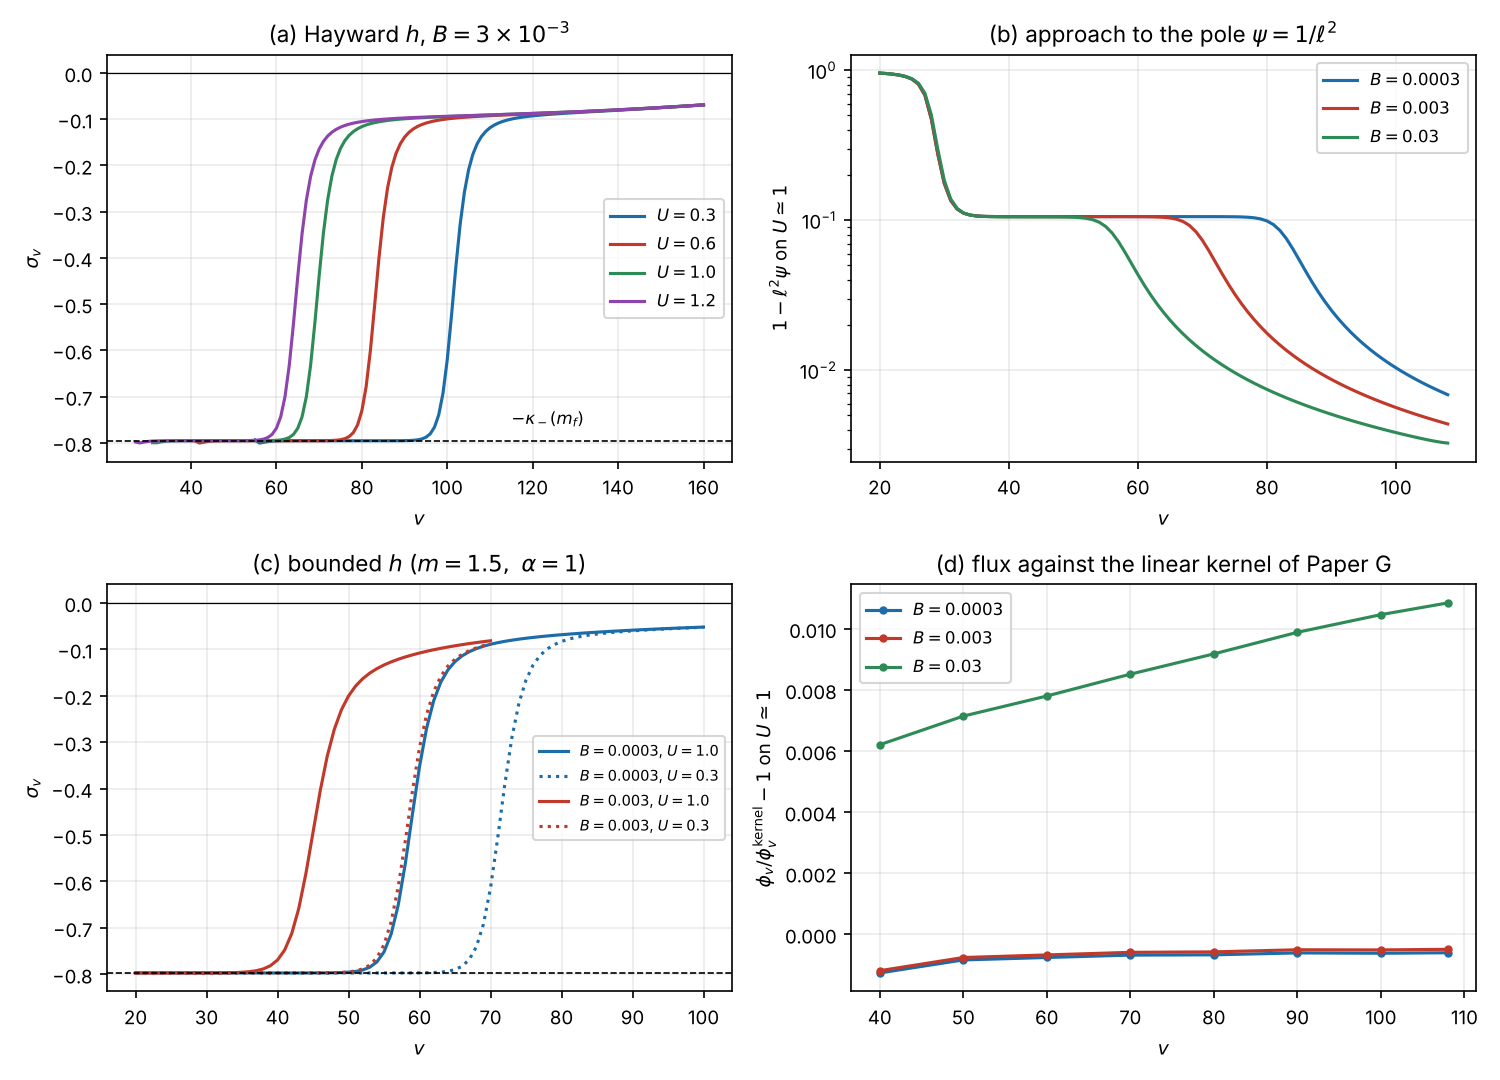
\includegraphics[width=\textwidth]{fig_eh.png}
\caption{Evolution from event-horizon-regular data. (a) $\sigma_v$ on four rays for the Hayward $h$, $B=3\times10^{-3}$ (Richardson--Romberg, converged window $v\le160$; the rays are plotted from the end of the static transition at $x\approx1$); dashed: $-\kappa_-(m_f)$. (b) $1-\ell^{2}\psi$ on $U\simeq1$ for three amplitudes; the drop near $v=20$--$35$ is the static transition from $\psi\approx0$ near the horizon to $\psi=1/r_-^{2}$. (c) Bounded $h$, $m=1.5$, $\alpha=1$: $\sigma_v$ on $U\simeq1$ (full) and $U\simeq0.3$ (dotted). (d) Ratio of the flux $\phi_v$ to the linear-response kernel of Paper~G~\citep{PaperG}, minus one, on $U\simeq1$.}
\label{fig:eh}
\end{figure}

\subsection{The flux through the interior against the linear kernel}

The scalar equation~\eqref{eq:phi} contains $h$ only through the metric. At linear order in $B$ the field propagates on the static background, which for the Hayward $h$ is the Hayward metric whatever the closure; the theory enters the flux only through the back-reaction, at $O(B^{2})$. The linear response of the static interior to the horizon flux and its kernel are therefore those of Paper~G. Table~\ref{tab:kernel} gives the ratio of the evolved flux $\phi_v$ on $U\simeq1$ to the kernel prediction. For $B=3\times10^{-4}$ and $3\times10^{-3}$ the ratio is $0.9992$--$0.9995$ for $v\ge60$ and the offsets from unity at the two amplitudes differ by at most $1.1\times10^{-4}$; for $B=3\times10^{-2}$ it is $1.0078$--$1.0108$, a nonlinear departure of $0.8$--$1.1\%$. The offset of $5$--$8\times10^{-4}$ at small $B$ is not a back-reaction effect (it does not scale with $B$) and is shared with the additive pipeline: the difference between the two evolutions is $-3.2\times10^{-4}$ at $B=3\times10^{-3}$ on the ray $U\simeq1$, so the additive flux departs from the kernel by about $3\times10^{-4}$, consistent with the $4\times10^{-4}$ of Papers~E and~G~\citep{PaperE,PaperG}. The difference of the two theories is quadratic in $B$: relative to the additive closure (same data, same four meshes; \texttt{cmp\_add\_B*.log}) the QTG flux differs by $-2.4\times10^{-4}$ to $-3.7\times10^{-4}$ at $B=3\times10^{-3}$ and by exactly $10^{-2}$ of that at $B=3\times10^{-4}$ (for $v=60$--$80$ on the four rays), i.e.\ by about $-(27\text{--}41)B^{2}$. This is the first quantity at which the theory is visible, and it is small. It stays small only until the front of Section~\ref{sec:front} reaches the ray: at $v=80$ on $U\simeq1$ the metric exponents of the two evolutions differ by $0.68$.

\begin{table}[ht]\centering\small
\caption{Flux $\phi_v$ of the evolved solution divided by the linear-response kernel prediction of Paper~G, ray $U\simeq1$ (\texttt{kernel\_ratio\_B*.log}).}\label{tab:kernel}
\begin{tabular}{lcccc}
\toprule
$B$ & $v=60$ & $v=80$ & $v=100$ & $v=108$\\\midrule
$3\times10^{-4}$ & 0.999244 & 0.999331 & 0.999383 & 0.999399\\
$3\times10^{-3}$ & 0.999328 & 0.999428 & 0.999492 & 0.999512\\
$3\times10^{-2}$ & 1.007802 & 1.009181 & 1.010465 & 1.010849\\\bottomrule
\end{tabular}
\end{table}

\subsection{The metric exponent}

Before the front, the interior is the static interior of the Hayward hole with the mass parameter reached on the horizon. On the rays where this regime lasts longest ($U\simeq0.3$) $\sigma_v$ is constant at a value that agrees with $-\kappa_-(m_f)$, with $m_f$ of~\eqref{eq:mf} and $\kappa_-(m)$ the surface gravity of the static Hayward hole with mass parameter $m$, and not with the static value $-\kappa_-(5)=-0.7956493$ (Table~\ref{tab:exp}; the plateau value is the median of the extrapolated $\sigma_v$ over the points $v\ge45$ with $\sigma_v<-0.79$). At $B=3\times10^{-2}$ the shift from the static value is $4.2\times10^{-4}$ and is reproduced to $1.3\times10^{-6}$. This is the property found in Paper~E~\citep{PaperE} for the additive closure, here in the theory whose static sector is the Hayward metric (\texttt{plateau\_m1\_B*.log}).

\begin{table}[ht]\centering\small
\caption{Plateau of $\sigma_v$ on $U\simeq0.3$ against $-\kappa_-(m_f)$, Hayward $h$.}\label{tab:exp}
\begin{tabular}{lcccc}
\toprule
$B$ & $m_f$ & $-\kappa_-(m_f)$ & plateau of $\sigma_v$ & difference\\\midrule
$3\times10^{-4}$ & 5.000001 & $-0.7956493$ & $-0.7956493$ & $-1.5\times10^{-10}$\\
$3\times10^{-3}$ & 5.000099 & $-0.7956534$ & $-0.7956534$ & $-4.1\times10^{-9}$\\
$3\times10^{-2}$ & 5.00996 & $-0.7960656$ & $-0.7960643$ & $+1.3\times10^{-6}$\\\bottomrule
\end{tabular}
\end{table}

\subsection{The front}
\label{sec:front}

At a time $v_f(U)$ the solution leaves the static regime: $\sigma_v$ rises from $-\kappa_-(m_f)$ to about $-0.1$, over $7.2$--$7.6$ units of $v$ between its $10\%$ and $90\%$ points on every ray and amplitude (Fig.~\ref{fig:eh}a; \texttt{width\_m1.log}), $1-\ell^{2}\psi$ falls from $1-r_-^{-2}=0.1057$ (Fig.~\ref{fig:eh}b), the generalized mass $m$ starts to grow, and $y$ and $g_\phi=\phi_u\phi_v/W$ grow from $\tfrac12$ and $<10^{-2}$ to $10^{7}$--$10^{8}$ (\texttt{late\_m1\_B*.log}). Defining $v_f$ by $\sigma_v=-0.4$, at $B=3\times10^{-3}$ it is $102.3,\,84.0,\,70.4,\,65.4$ on $U\simeq0.3,\,0.6,\,1.0,\,1.2$, and on $U\simeq1$ it is $83.5,\,70.4,\,57.3$ for $B=3\times10^{-4},\,3\times10^{-3},\,3\times10^{-2}$: a delay of $13.1$ per decade of $1/B$, i.e.\ $5.7$ per $e$-fold (\texttt{front\_m1\_B*.log}). The front is not at a fixed Kruskal value $x=Ue^{\kappa_+v}$: $x_f=45,\,37,\,31,\,30$ on the four rays at $B=3\times10^{-3}$, and $60,\,31,\,16.5$ on $U\simeq1$ for the three amplitudes. We have not derived the delay; its logarithmic dependence on $B$ is that expected for a quantity that grows exponentially from an initial value $\propto B$ or $B^{2}$ (the finite-advanced-time singularity of the interior-data ray, Appendix~\ref{sec:num}, has $12.3$ per decade).

\subsection{Behind the front}

Table~\ref{tab:front} follows $U\simeq1$ for $B=3\times10^{-3}$ from the run to $v_1=200$, with the inter-level differences that define the window. Behind the front: (1) $r$ stays within $3\times10^{-6}$ of $r_-=1.057475$; (2) $\psi\to1/\ell^{2}$ from below, algebraically: $1-\ell^{2}\psi=\psi r^{3}/(2m)$ exactly (from $h=2m/r^{3}$), so with $r\simeq r_-$ one has $(1-\ell^{2}\psi)\,m\to\tfrac12r_-^{3}/\ell^{2}=0.59$ (Table~\ref{tab:front}), and since $m$ grows linearly in the window, $\mathrm{d}m/\mathrm{d}v=3.7\to4.1$, the pole is approached as $1/v$ and never reached; (3) $\mathrm{d}m/\mathrm{d}v=8\pi r^{2}y\phi_v^{2}$ with $y\phi_v^{2}\simeq0.13$--$0.145$ nearly constant ($y$ grows as $\phi_v^{2}$ decays); (4) $\sigma_v$ rises monotonically from $-0.094$ at $v=100$ to $-0.056$ at $v=180$, with an increment of $6.3$--$6.5\times10^{-4}$ per unit $v$ over $160\le v\le190$ (the same on all four rays); it has not reached zero (and does not in the extended runs of Section~\ref{sec:endpoint}).

\begin{table}[ht]\centering\small
\caption{Hayward $h$, $B=3\times10^{-3}$, ray $U\simeq1$ (run to $v_1=200$, extrapolated over four meshes). $\delta\sigma_v$ and $\delta z$: difference between the top two levels of the Romberg table (absolute for $\sigma_v$, relative for $z=1-\ell^{2}\psi$); $\mathrm{d}m/\mathrm{d}v$ by central differences over $\pm5$; $y\phi_v^{2}$ as defined in the text (\texttt{endpoint\_m1\_B0.003\_v200.log}).}\label{tab:front}
\begin{tabular}{rcccccccc}
\toprule
$v$ & $\sigma_v$ & $\delta\sigma_v$ & $z$ & $\delta z/z$ & $m$ & $\mathrm{d}m/\mathrm{d}v$ & $zm$ & $y\phi_v^{2}$\\\midrule
80 & $-0.1159$ & $1.9\!\times\!10^{-9}$ & $1.77\!\times\!10^{-2}$ & $5.5\!\times\!10^{-8}$ & 32.8 & 3.21 & 0.581 & 0.116\\
100 & $-0.0941$ & $2.3\!\times\!10^{-10}$ & $5.65\!\times\!10^{-3}$ & $2.6\!\times\!10^{-7}$ & 104.1 & 3.72 & 0.588 & 0.133\\
120 & $-0.0876$ & $4.0\!\times\!10^{-9}$ & $3.28\!\times\!10^{-3}$ & $1.3\!\times\!10^{-7}$ & 179.9 & 3.84 & 0.589 & 0.137\\
140 & $-0.0796$ & $6.9\!\times\!10^{-8}$ & $2.29\!\times\!10^{-3}$ & $4.1\!\times\!10^{-6}$ & 257.5 & 3.92 & 0.590 & 0.139\\
160 & $-0.0688$ & $1.4\!\times\!10^{-6}$ & $1.75\!\times\!10^{-3}$ & $2.2\!\times\!10^{-4}$ & 336.7 & 4.00 & 0.590 & 0.142\\
180 & $-0.0561$ & $3.4\!\times\!10^{-5}$ & $1.41\!\times\!10^{-3}$ & $8.6\!\times\!10^{-3}$ & 417.4 & 4.07 & 0.590 & 0.145\\\bottomrule
\end{tabular}
\end{table}

The generalized mass of the ray therefore inflates without bound (linearly in $v$ in the window), $\psi$ approaches the pole, and the Misner--Sharp mass $M=\tfrac12r^{3}\psi$ stays at $\tfrac12r_-^{3}/\ell^{2}\cdot\psi\approx0.59$. This is the inflation of the generalized mass of Section~\ref{sec:classes}, with a front and a rate that the characteristic data of Appendix~\ref{sec:num} could not show. The mass law is verified on the extrapolated rays: over $[80,90]$, $[90,100]$ and $[100,108]$ on $U\simeq1$ the mass increment equals the trapezoid integral of $8\pi r^{2}y\phi_v^{2}$ (samples every unit of $v$) to $1.1\times10^{-4}$, $2.1\times10^{-5}$ and $7.5\times10^{-6}$ ($B=3\times10^{-3}$; \texttt{masslaw\_m1\_B*.log}), with the larger values, $1.3\times10^{-2}$ over $[60,70]$ and $1.1\times10^{-3}$ over $[70,80]$, in the windows where the front passes and the trapezoid rule at $\Delta v=1$ is the limit; at $B=3\times10^{-2}$ it holds to $6.4\times10^{-4}$ and $5.9\times10^{-5}$ in $[60,70]$ and $[70,80]$ and degrades beyond $v=100$, outside the converged window.

\subsection{Behind the front the solution is slaved to the interior flux}
\label{sec:slave}

The following are properties of the evolved solution for $B=3\times10^{-3}$, from snapshots on rows $v=\mathrm{const}$ at $v=100,\,150,\,190$ or $200$ ($h_s=0.05$, $h_v=0.003125$ or $0.0125$, not extrapolated; \texttt{slaving.log}, \texttt{slaving\_prof.log}, \texttt{rho\_check.log}); they are observations, and the consequences below are derived from them. With $x=Ue^{\kappa_+v}$ and $\rho=-r_v$:
\begin{enumerate}
\item[(a)] \emph{The flux is independent of $u$.} $\phi_v$ varies by $3\times10^{-6}$ (max$-$min over mean) across $10\le x\le2\times10^{4}$ at the three times. We call it $\Phi(v)$. It is the flux through the interior of the linear response of Paper~G: $\Phi_{\rm PDE}/\Phi_{\rm kernel}=1.0001$ at $v=100$ and $1.0006$ for $150\le v\le250$ (\texttt{gpred\_final.log}), the $O(B^{2})$ difference of Table~\ref{tab:kernel}.
\item[(b)] \emph{$\rho$ is independent of $u$ behind the edge of the plateau.} Between $x=40$ and $x\gtrsim200$ it varies by $1\times10^{-4}$, $2\times10^{-3}$ and $2\times10^{-2}$ (relative) at $v=100,\,150,\,200$ (the variation grows with $v$; a difference of $10^{-4}$ in $\rho_v/\rho$ between two values of $x$, which is the size of the $h_s$-systematic of Section~\ref{sec:cy} and of the spread in~(c), accumulates to $1\%$ over $100$ units of $v$).
\item[(c)] \emph{The Raychaudhuri equation} \eqref{eq:ray} reads $\rho_v=\sigma_v\rho+S$, $S=4\pi rc_1\phi_v^{2}$, so that $\rho_v/\rho=\sigma_v+S/\rho$ at every point. This sum is independent of $x$: $-0.0922\pm1\times10^{-4}$ for $30\le x\le200$ at $v=100$, $-0.07438\pm2\times10^{-5}$ for $40\le x\le2300$ at $v=150$, $-0.0432\pm1\times10^{-4}$ for $60\le x\le10^{4}$ at $v=200$ (\texttt{slaving\_prof.log}). Behind the front ($x\ge2x_f$) $c_1=z^{2}\lesssim10^{-4}$, so $S/\rho\lesssim5\times10^{-3}$ and $\sigma_v=\rho_v/\rho$ up to that: the metric exponent is the logarithmic derivative of $\rho$. In the plateau ($30\lesssim x\lesssim x_f$) $\sigma_v=-\kappa_-(m_f)$ and $S/\rho=0.70$--$0.73$.
\item[(d)] \emph{An exact identity.} By the definition of $\psi$, $y\rho=\beta\equiv(\psi r^{2}-1)/4$ (to $10^{-6}$, \texttt{slaving.log}). With $W=-r_u/y$ this gives $\sigma_v=\rho_v/\rho+r_{uv}/r_u-\beta_v/\beta$ identically; the last two terms are $-9\times10^{-5}$ at $v=200$ ($\sigma_v=-0.0438$) and decrease faster than $1/v$ (\texttt{rho\_check.log}).
\end{enumerate}
Since $\rho_v/\rho$ takes the same value at every $x$ in the region covered by (b), it can be evaluated where the equation is simplest, in the plateau, where $\sigma_v=-\kappa_-$ and $c_1=c_1^{\rm II}=(1-1/r_-^{2})^{2}$ are constants and $r=r_-$:
\begin{equation}
\rho_v=-\kappa_-\rho+S^{\rm II}(v),\qquad S^{\rm II}=4\pi r_-c_1^{\rm II}\,\Phi(v)^{2},\qquad \sigma_v\;\to\;G(v)\equiv\frac{S^{\rm II}}{\rho}-\kappa_-.
\label{eq:slave}
\end{equation}
The amplitude of $\Phi$ cancels in $G$: it depends on the shape of $\Phi(v)$ alone, and so does not depend on $B$. Two further consequences follow from the exact mass law~\eqref{eq:mlaw} and (d): $\mathrm{d}m/\mathrm{d}v=8\pi r^{2}y\phi_v^{2}=2r\beta\,(S^{\rm II}/\rho)/c_1^{\rm II}$, that is
\begin{equation}
\frac{\mathrm{d}m}{\mathrm{d}v}=\frac{2r\beta}{c_1^{\rm II}}\,\bigl(\kappa_-+G\bigr)\;\longrightarrow\;\frac{2r_-\beta_\infty\kappa_-}{c_1^{\rm II}}=4.45,\qquad \beta_\infty=\frac{r_-^{2}-1}{4},
\label{eq:dm}
\end{equation}
and $zm=\psi r^{3}/2$ exactly. \emph{Tests.} With $\Phi$ the kernel flux of Paper~G, the solution of~\eqref{eq:slave} ($\rho$ is the convolution of $S^{\rm II}$ with $e^{-\kappa_-v}$ from $v=20$; \texttt{gpred\_q.py}) predicts $G(v)$ with no further input. Table~\ref{tab:end} gives it beside the extrapolated $\sigma_v$, and Table~\ref{tab:k} for other amplitudes and tail exponents. For $B=3\times10^{-3}$ the difference $\sigma_v-G$ is $-2.1\times10^{-3}$ at $v=100$ (the transient after the front has not died out: the front is only $\sim50$ units of $v$ earlier on this ray), $-3.2\times10^{-4}$ at $150$ and $-2.2\times10^{-4}$ at $200$, $-2.0\times10^{-4}$ at $250$, where $1.6\times10^{-4}$ is the $h_s$-systematic of Section~\ref{sec:cy}; after the $h_s\to0$ extrapolation the residual is $-7.5\times10^{-5}$, $-5.6\times10^{-5}$ and $-4.3\times10^{-5}$ at $v=180,\,200,\,220$ ($0.13\%$ of $G$; \texttt{hs\_extrap.log}), the size of the $0.06\%$ difference of the PDE flux from the kernel in~(a). The closed form~\eqref{eq:dm}, with the local $\beta$ and the extrapolated $\sigma_v$, gives $\mathrm{d}m/\mathrm{d}v$ to $0.8\%$ ($3.693$ against $3.730$ at $v=100$, $4.135$ against $4.162$ at $v=200$; Table~\ref{tab:end}). In the bounded model the relation $\sigma_v=\rho_v/\rho$ holds with $\sigma_v-\rho_v/\rho=-3.6\times10^{-4},\,-1.8\times10^{-4},\,-1.0\times10^{-4}$ at $v=95,\,110,\,125$ ($B=3\times10^{-4}$, $m=1.5$; $\sigma_v=-0.0552,\,-0.0470,\,-0.0411$), while $2\,\mathrm{d}\ln|\Phi|/\mathrm{d}v$ is within $2$--$3\%$ of $\rho_v/\rho$ (\texttt{bounded\_aniso.log}); we did not build the bounded-$h$ kernel.

\subsection{The endpoint}
\label{sec:endpoint}

\emph{What the extended runs show.} With the remedy of Section~\ref{sec:cy} the run for $B=3\times10^{-3}$ is accurate to $v=300$ (inter-level difference of $\sigma_v$ at most $9\times10^{-6}$) and usable to $v\simeq320$ ($2\times10^{-4}$); eight levels $h_v=0.05,\ldots,3.9\times10^{-4}$ from two runs of the same problem (\texttt{genq2\_hs0.05\_m1\_B0.003\_k1.5\_v400.json} and \texttt{\_v360.json}, whose rays coincide to $10^{-7}$ in $U$; the convergence ratio of successive levels is $4.0$ across the two files, \texttt{merge\_levels.py}) are used (Table~\ref{tab:end}). $\sigma_v$ increases monotonically from $-0.094$ at $v=100$ and does not reach zero: it is $-0.0182$ at $v=300$, whereas the linear continuation from the end of the earlier window ($6.4\times10^{-4}$ per unit $v$ at $v=180$) reached zero near $v\simeq270$. The increment decreases instead: $\mathrm{d}\sigma_v/\mathrm{d}v=6.4\times10^{-4}$ at $v=180$, $3.4\times10^{-4}$ at $230$ and $1.2\times10^{-4}$ at $280$. The product $v\sigma_v$ has a minimum $-11.2$ near $v=150$ and rises to $-5.47$ at $v=300$ (and to $-5.58$ at $v=290$ for $B=3\times10^{-4}$, \texttt{endpoint\_B0.0003.log}), toward the value $-5$ derived below. The generalized mass has $\mathrm{d}m/\mathrm{d}v=4.30$ at $v=280$, the closed form~\eqref{eq:dm} giving $4.29$ (it tends to $4.45$), and $zm=\tfrac12\psi r^{3}$ stays at $0.59$. The curvature invariant increases monotonically after the front (Table~\ref{tab:end}; Section~\ref{sec:curv}).

\begin{table}[ht]\centering\small
\caption{Hayward $h$, $B=3\times10^{-3}$, $k=3/2$, $m=5$, ray $U\simeq1$ ($h_s=0.05$; Romberg in $h_v^{2}$ over the finest levels that are finite $30$ units of $v$ beyond the point, Section~\ref{sec:cy}; \texttt{endpoint\_B0.003\_merged.log}). $\delta\sigma_v$: difference between the top of the table and the extrapolation from the finest $K-1$ levels (it does not include the $h_s$-systematic of $1.6\times10^{-4}$). $G$: prediction of Eq.~\eqref{eq:slave} from the kernel flux. $\mathrm{d}m/\mathrm{d}v$ by central differences over $\pm5$; ``closed'': Eq.~\eqref{eq:dm} with the local $\beta$ and the measured $\sigma_v$. $K$: Kretschmann invariant in units $\ell^{-4}$.}\label{tab:end}
\begin{tabular}{rcccccccc}
\toprule
$v$ & $\sigma_v$ & $\delta\sigma_v$ & $G$ & $v\sigma_v$ & $z$ & $\mathrm{d}m/\mathrm{d}v$ & closed & $K$\\\midrule
100 & $-$0.094251 & $3\!\times\!10^{-11}$ & $-$0.092186 & $-$9.425 & $5.64\!\times\!10^{-3}$ & 3.730 & 3.693 & $1.1\!\times\!10^{25}$\\
120 & $-$0.087733 & $2\!\times\!10^{-11}$ & $-$0.087031 & $-$10.528 & $3.27\!\times\!10^{-3}$ & 3.848 & 3.816 & $1.7\!\times\!10^{25}$\\
140 & $-$0.079755 & $3\!\times\!10^{-11}$ & $-$0.079363 & $-$11.166 & $2.29\!\times\!10^{-3}$ & 3.926 & 3.896 & $6.0\!\times\!10^{25}$\\
160 & $-$0.068968 & $6\!\times\!10^{-11}$ & $-$0.068687 & $-$11.035 & $1.75\!\times\!10^{-3}$ & 4.004 & 3.976 & $2.5\!\times\!10^{26}$\\
180 & $-$0.056255 & $2\!\times\!10^{-10}$ & $-$0.056017 & $-$10.126 & $1.41\!\times\!10^{-3}$ & 4.086 & 4.058 & $8.6\!\times\!10^{26}$\\
200 & $-$0.043998 & $4\!\times\!10^{-10}$ & $-$0.043779 & $-$8.800 & $1.18\!\times\!10^{-3}$ & 4.162 & 4.135 & $2.2\!\times\!10^{27}$\\
220 & $-$0.034253 & $1\!\times\!10^{-9}$ & $-$0.034044 & $-$7.536 & $1.01\!\times\!10^{-3}$ & 4.222 & 4.195 & $4.3\!\times\!10^{27}$\\
240 & $-$0.027494 & $3\!\times\!10^{-9}$ & $-$0.027293 & $-$6.599 & $8.82\!\times\!10^{-4}$ & 4.264 & 4.238 & $6.5\!\times\!10^{27}$\\
260 & $-$0.023090 & $5\!\times\!10^{-9}$ & $-$0.022894 & $-$6.003 & $7.82\!\times\!10^{-4}$ & 4.292 & 4.266 & $8.7\!\times\!10^{27}$\\
280 & $-$0.020206 & $4\!\times\!10^{-8}$ & $-$0.020014 & $-$5.658 & $7.02\!\times\!10^{-4}$ & 4.310 & 4.285 & $1.1\!\times\!10^{28}$\\
300 & $-$0.018223 & $9\!\times\!10^{-6}$ & $-$0.018030 & $-$5.467 & $6.37\!\times\!10^{-4}$ & 4.372 & 4.299 & $1.3\!\times\!10^{28}$\\
\bottomrule
\end{tabular}
\end{table}

\emph{Other amplitudes and tail exponents.} Table~\ref{tab:k} compares $\sigma_v$ with the kernel prediction $G$ for $k=\tfrac12,\,\tfrac32,\,3$ and for $B=3\times10^{-4},\,3\times10^{-3},\,3\times10^{-2}$ (runs \texttt{genq2\_hs0.05\_m1\_B*\_k*\_v*.json}, four levels each, Romberg as above; \texttt{ktable.log}). After the transient, $\sigma_v-G=-(1.9$--$3.0)\times10^{-4}$ for all five cases at $v\ge200$ ($-(2.7$--$4.4)\times10^{-4}$ at $v=150$) (it is the $h_s$-systematic $-1.6\times10^{-4}$ and the $O(B^{2})$ flux difference of Section~\ref{sec:slave}), although $\sigma_v$ itself differs by a factor $5.8$ between $k=\tfrac12$ and $k=3$ at $v=200$. For $k=3$ the tail is steep, $\Phi$ is dominated by the exponential of the kernel for $v\lesssim(k+1)/\kappa_+=82$ and well beyond, and $\sigma_v$ sits on a plateau $-0.098$ to $-0.099$ at $120\le v\le190$, which is $-2\kappa_+=-0.0979$ (the kernel prediction is still $-0.0979$ at $v=200$ and reaches the power law, $-0.0419$ at $v=400$, only at $v\gtrsim300$). For $k=\tfrac12$, $v\sigma_v=-4.49,\,-3.75,\,-3.36,\,-3.22$ at $v=100,\,150,\,200,\,290$ and tends to $-3=-(2k+2)$ (the kernel gives $-3.31,\,-3.09,\,-3.03,\,-3.02$ at $200,\,400,\,10^{3},\,2\times10^{3}$). The windows: $k=\tfrac12$ is accurate to $v\simeq290$; $k=3$ to $v\simeq190$ (the first non-finite sample is $196,\,225,\,253,\,281$ at $h_v=0.025,\ldots,0.003125$, shifted by $-37.6$ with respect to Eq.~\eqref{eq:vb}, whose constant depends on $k$); $B=3\times10^{-2}$ to $v\simeq160$.

\begin{table}[ht]\centering\small
\caption{$\sigma_v$ on $U\simeq1$ ($h_s=0.05$) and its difference from the kernel prediction $G$ of Eq.~\eqref{eq:slave} (in units of $10^{-4}$), for the tail exponents $k=\tfrac12,\tfrac32,3$ and amplitudes $B$ (\texttt{ktable.log}); --: beyond the accurate range. The limiting values $-(2k+2)/v$ are $-0.010,\,-0.017,\,-0.028$ at $v=290$ for $k=\tfrac12,\tfrac32,3$. In all cases the $h_s$-systematic is $-1.6\times10^{-4}$.}\label{tab:k}
\begin{tabular}{rccccc}
\toprule
 & $k=\tfrac12$ & \multicolumn{3}{c}{$k=\tfrac32$} & $k=3$\\
$v$ & $B=3\!\times\!10^{-3}$ & $3\!\times\!10^{-4}$ & $3\!\times\!10^{-3}$ & $3\!\times\!10^{-2}$ & $3\!\times\!10^{-3}$\\\midrule
100 & $-0.04488$ ($-16$) & $-0.09908$ ($-69$) & $-0.09425$ ($-21$) & $-0.09306$ ($-8.7$) & $-0.10104$ ($-22$)\\
150 & $-0.02497$ ($-3.7$) & $-0.07482$ ($-4.4$) & $-0.07471$ ($-3.2$) & $-0.07469$ ($-3.1$) & $-0.09839$ ($-2.7$)\\
200 & $-0.01681$ ($-2.4$) & $-0.04402$ ($-2.4$) & $-0.04400$ ($-2.2$) & -- & $-0.09812$ ($-1.9$)\\
250 & $-0.01295$ ($-2.2$) & $-0.02507$ ($-2.2$) & $-0.02505$ ($-2.0$) & -- & --\\
290 & $-0.01111$ ($-2.8$) & $-0.01923$ ($-3.0$) & $-0.01913$ ($-1.9$) & -- & --\\\bottomrule
\end{tabular}
\end{table}

\emph{Asymptotics of the slaved description.} Eq.~\eqref{eq:slave} fixes the late behavior once $\Phi(v)$ is known. (i) \emph{Sign.} If $S^{\rm II}\propto\Phi^{2}$ decreases, then $\rho(v)=\int_{v_0}^{v}S^{\rm II}(v')e^{-\kappa_-(v-v')}\mathrm{d}v'\ge S^{\rm II}(v)/\kappa_-$ and $G=S^{\rm II}/\rho-\kappa_-\le0$: no zero crossing. The kernel flux $|\Phi|$ is strictly decreasing on the unit grid $20\le v\le1200$ for $k=\tfrac12,1,\tfrac32,2,3$, with $|\Phi(v+1)/\Phi(v)|<0.9988$ (\texttt{phi\_monotone.py}, \texttt{logs/phi\_monotone.log}), and the exact identity~(d) adds the term $-\beta_v/\beta<0$. (ii) \emph{Rate.} The kernel of Paper~G tends to $K(t)\to R_1e^{-\kappa_+t}$, so $\Phi(v)=\int K(v-v')j(v')\mathrm{d}v'\to(R_1/\kappa_+)\,j(v)\,[1+O((k+1)/\kappa_+v)]$, with $j\propto v^{-(k+1)}$ the horizon flux of the tail $\phi\propto v^{-k}$. Then $\rho\to S^{\rm II}/\kappa_-$ and
\begin{equation}
\sigma_v\;\to\;\frac{\mathrm{d}\ln S^{\rm II}}{\mathrm{d}v}=2\frac{\mathrm{d}\ln|\Phi|}{\mathrm{d}v}\;\to\;-\frac{2(k+1)}{v}=-\frac5v\quad(k=\tfrac32),
\label{eq:asym}
\end{equation}
with corrections of relative size $(k+1)/(\kappa_+v)$, which is $0.26$ at $v=200$: the approach is slow. The kernel prediction for $vG$ ($k=\tfrac32$) is $-8.76$ at $v=200$, $-5.16$ at $400$, $-5.05$ at $10^{3}$ and $-5.03$ at $2\times10^{3}$ (\texttt{gpred\_final.log}), against $-8.80$ at $200$ and $-5.47$ at $300$ in Table~\ref{tab:end}. (iii) \emph{Consequences} (all in the slaved description, as $v\to\infty$): $W=-r_u\rho/\beta\propto\rho\propto v^{-(2k+2)}$, with $r_u$ independent of $v$ ($\partial_v\ln|r_u|=-1.4\times10^{-7}$ at $v=200$, \texttt{rho\_check.log}), so the affine parameter $\lambda=\int W\,\mathrm{d}v$ of the ingoing null geodesic at fixed $u$ (along which $W\,\mathrm{d}v/\mathrm{d}\lambda$ is constant, since $g_{uv}k^{v}$ is conserved) has a finite range to $v=\infty$, with remaining length $\Delta\lambda\propto v^{-(2k+1)}$; $m\simeq4.45\,(v-v_0)$ in the limit ($\mathrm{d}m/\mathrm{d}v=4.3$ in the window) and $z=\psi r^{3}/2m\propto1/(v-v_0)$ with $v_0\approx85$ (from $m(v)$, Section~\ref{sec:curv2}); $\psi\to1/\ell^{2}$, $r\to r_-$ and $\sigma_v\to0^{-}$; and the invariant is $K\simeq16\Sigma^{2}\propto z^{6}\Phi^{-4}$, which in this description tends to $v^{4k-2}$ ($=v^{4}\propto\Delta\lambda^{-1}$ for $k=3/2$; we regard this as a conjecture about the endpoint, supported by the structure but not reached by the simulation; the structural relation $Kz^{-6}\Phi^{4}=\mathrm{const}$ holds to a factor $1.7$--$2.2$ over $100\le v\le280$ while $K$ changes by $10^{3}$, \texttt{curv\_hv.log}, \texttt{curv\_hv\_B0.0003.log}). The offset $v_0$ delays the asymptotic exponents: the local exponent of $z$ is $-1.43$ at $v=280$ and $-1.29$ at $380$ and that of $K$ is $-6v/(v-v_0)+2|vG|$ (Eq.~\eqref{eq:kslope}), which is $2.5$ at $v=300$ and $3.4$ at $v=10^{3}$; it was measured to be $2.5$ on $300\le v\le380$ with code~B (Section~\ref{sec:curv2}; $2.1$ at $v=280$ for $B=3\times10^{-4}$ and $4.2$ at $v=240$ for $B=3\times10^{-3}$ with code~A) and returns to $4$ only for $v\gtrsim10^{3}$. For the exponent $k=\tfrac12$ the same relation gives $K\propto v^{0}$: in the run $K$ decreases after the front ($2.1\times10^{21}$ at $v=100$, $3.0\times10^{19}$ at $v=290$, \texttt{endpoint\_k0.5.log}), the sign that the structure predicts at these $v$ and an illustration that the growth of the curvature depends on the tail; for $k=3$ it rises steeply ($4.9\times10^{25}$ at $v=100$, $3.8\times10^{29}$ at $190$).

\emph{What is and is not shown.} Shown: the structure (a)--(d) of Section~\ref{sec:slave} between $v=100$ and $v\simeq300$ for $B=3\times10^{-3}$, with a second code to $v\simeq380$ (Sections~\ref{sec:code2} and~\ref{sec:curv2}); that the prediction~\eqref{eq:slave} reproduces $\sigma_v$ to the level of the numerical systematic ($2\times10^{-4}$, $0.13\%$ after $h_s\to0$ for $180\le v\le230$) for three tail exponents and three amplitudes; that $\sigma_v$ approaches zero from below with a decreasing rate; and the monotonic growth of $K$ for $k\ge\tfrac32$. Not shown: anything about $v\gtrsim1400$ (and, with codes A and B, $v\gtrsim400$), which rests on the continuation of the slaved structure and of the kernel (Eq.~\eqref{eq:asym}) and is not a simulation. In particular a finite affine range to $v=\infty$ (the simulated $W\propto v^{-5.1}$ is consistent with it) and $K\propto v^{4k-2}$ (not reached: local slope $2.5$ at $v=300$--$380$ and $3.64$ at $1400$, Section~\ref{sec:curv3}) are predictions of the effective description; we do not claim that the Cauchy horizon of the hole is a singularity of a given strength, only that within this description the invariant diverges as a power of $v$ for $k>\tfrac12$. The description itself is classical and ceases to apply when $K\gg\ell^{-4}$ (Section~\ref{sec:open}), which is the case already at $10^{25}$.

\subsection{Curvature}
\label{sec:curv}

The Kretschmann invariant of the metric $-W\,du\,dv+r^{2}d\Omega^{2}$ is, for any $h$ and in terms of the solved fields (Appendix~\ref{app:curv}),
\begin{align}
K&=(4\Sigma)^{2}+8\,\frac{H_{ab}H^{ab}}{r^{2}}+4\psi^{2},\label{eq:kret}\\
\Sigma&=\frac{\sigma_{uv}}{W}=\frac{\psi}{2}-c_2-8\pi c_1g_\phi+64\pi^{2}c_3g_\phi^{2},\qquad
\frac{H_{ab}H^{ab}}{r^{2}}=128\pi^{2}c_1^{2}g_\phi^{2}+\frac{Q^{2}}2,\nonumber
\end{align}
with $g_\phi=\phi_u\phi_v/W$ and $H_{ab}=\nabla_a\nabla_br$. For $g_\phi=0$ and the Hayward $h$ at the pole ($\psi=1/\ell^{2}$, $c_2=0$, $Q=-2/\ell^{2}$) this gives $K=24\,\ell^{-4}$, the de Sitter value, and for $h=\psi$ it gives $48M^{2}/r^{6}$; on the static Hayward and bounded interiors it agrees with $f''^{2}+4f'^{2}/r^{2}+4(1-f)^{2}/r^{4}$ to $3.4\times10^{-7}$ and $7.2\times10^{-8}$ (finite differences; \texttt{check\_curv\_static.log}).

Behind the front the static part stays at $O(\ell^{-4})$ and the invariant is carried by the flux terms. At $B=3\times10^{-3}$ the maximum of $K$ over the sampled $v$ is $2.9\times10^{32},\,4.7\times10^{29},\,2.8\times10^{27}$ ($\ell^{-4}$) on $U\simeq0.3,\,0.6,\,1.0$, at the passage of the front ($v=103,\,85,\,72$). On $U\simeq1$, $K=1.4\times10^{26}$ at $v=80$, falls to $1.1\times10^{25}$ at $v=100$, and then rises again: $1.7\times10^{25}$, $5.8\times10^{25}$, $2.4\times10^{26}$ at $v=120,\,140,\,160$ (\texttt{curv\_m1\_B*.log}, \texttt{late\_m1\_B0.003\_v200.log}). At $v=100$ the terms of $\Sigma$ on $U\simeq1$ are $\psi/2=0.50$, $-c_2=-0.025$, $-8\pi c_1g_\phi=-4.8\times10^{4}$ and $64\pi^{2}c_3g_\phi^{2}=8.3\times10^{11}$ (\texttt{curv\_terms\_m1\_B0.003.log}): the invariant is $\simeq16\Sigma^{2}$ with $\Sigma$ dominated by the $c_3$ term, which is specific to this theory (it is absent for $h=\psi$) and is fixed by the compatibility condition (Section~\ref{sec:checks}(e)). The bound on the curvature of the static Hayward metric does not extend to the dynamical solution with flux. A curvature of $10^{25}\ell^{-4}$ means a curvature radius $10^{-6}\ell$; for any $\ell$ above the Planck length the classical description by this theory is not reliable there, and the solution should be read as the classical evolution of the theory, not as a prediction for the physical hole. We note also that the size of $K$ rests on the $c_3$ term of~\eqref{eq:suv}: it is the field equation of the reduced action (Section~\ref{sec:checks}(f), exact in rational arithmetic) and agrees with the compatibility condition ($3\times10^{-12}$); the second-order convergence of the Raychaudhuri residuals and the $r_{uv}$ residual through the front (Section~\ref{sec:cy}(iii)) test the scheme, and there is no numerical test of the term in the region behind the front. \emph{Later times.} With the extended runs of Section~\ref{sec:cy}, $K$ on $U\simeq1$ ($B=3\times10^{-3}$) keeps rising after $v=160$: $1.4\times10^{27}$, $4.3\times10^{27}$, $6.5\times10^{27}$ at $v=190,\,220,\,240$ and $1.3\times10^{28}$ at $300$ (Table~\ref{tab:end}); its local logarithmic slope $\mathrm{d}\ln K/\mathrm{d}\ln v$ is $10.9$ at $v=160$ and $4.2$ at $v=240$. For $B=3\times10^{-4}$ (front later) $K=3.6\times10^{34}$ at $v=100$, falls to $1.1\times10^{34}$ at $120$ and rises to $1.7\times10^{36}$ at $v=290$, with slope $9.1$ at $v=170$ and $2.1$ at $v=280$ (\texttt{curv\_hv\_B0.0003.log}). Behind the front the slaved structure of Section~\ref{sec:slave} gives $K\simeq16\Sigma^{2}\propto z^{6}\Phi^{-4}$ (the combination $Kz^{-6}\Phi^{4}$ changes by a factor $1.7$--$2.2$ over $100\le v\le280$ while $K$ changes by $10^{3}$), so the growth rate depends on the tail exponent $k$ through $\Phi\propto v^{-(k+1)}$ (Section~\ref{sec:endpoint}).

\subsection{The curvature invariant and the tidal integrals to \texorpdfstring{$v=380$}{v=380}}
\label{sec:curv2}

Code~B (Section~\ref{sec:code2}, $h_s=0.05$, $h_v=0.0125$, $B=3\times10^{-3}$, $k=\tfrac32$, ray $U\simeq1$) allows $K$ to be followed from $v\simeq300$ to $v\simeq380$ (change from the next coarser level $2.4\times10^{-3}$ at $v=300$, $1.8\times10^{-2}$ at $340$, $0.15$ at $380$, i.e.\ an error of about $1\%$ at $380$; \texttt{tidal\_v600.log}). The scripts are \texttt{kstudy.py} and \texttt{tidal.py}; all numbers below are from them.

\paragraph{The invariant.} $K=1.09\times10^{25},\,2.17\times10^{27},\,1.26\times10^{28},\,1.98\times10^{28}$ and $2.27\times10^{28}\ell^{-4}$ at $v=100,\,200,\,300,\,360$ and $380$. Code~A at $h_s=0.05$ gives $K$ higher by $3\%$ ($1.12\times10^{25}$, $2.22\times10^{27}$, $1.29\times10^{28}$ at $100$, $200$, $300$): this is its $h_s$-systematic, and the $K$ column of Table~\ref{tab:end}, and the values quoted in Sections~\ref{sec:endpoint} and~\ref{sec:curv}, carry it (it does not affect logarithmic slopes at the level used here). At $v=340$ the terms of $\Sigma$ are $\psi/2=0.4997$, $-c_2=-2.4\times10^{-3}$, $-8\pi c_1g_\phi=-9.4\times10^{4}$ and $64\pi^{2}c_3g_\phi^{2}=3.3\times10^{13}$: the last is $1+3\times10^{-9}$ times $\Sigma$, and the other two terms of~\eqref{eq:kret} are of relative size $10^{-17}$ and smaller. For the Hayward $h$, $c_3=h''/h'^{3}=2z^{3}$ ($\ell=1$), so $K\simeq(512\pi^{2})^{2}z^{6}g_\phi^{4}$ to better than $10^{-8}$: the curvature of the dynamical solution is carried entirely by the $\phi_u^{2}\phi_v^{2}$ term, which the minimally coupled scalar sources through the quartic part of the theory. (Behind the front $\Omega=\mathcal R+2\eta+2\psi\simeq4\Sigma\ge8\times10^{11}$, so $I_{C^{2}}=\Omega^{2}/3$ and the denominators of the lifts of Section~\ref{sec:checks}(g) do not vanish.) The local slope $\mathrm d\ln K/\mathrm d\ln v$ is $10.9$ at $v=160$, $7.9$ at $200$, $4.2$ at $240$, $3.2$ at $260$, $2.7$ at $280$, $2.5$ at $300$, and then $2.47,\,2.48,\,2.50,\,2.45$ at $v=320,\,340,\,360,\,380$ (centered differences over $\pm10$): in the simulated range $K$ does \emph{not} follow $v^{4k-2}=v^{4}$, and its slope has a maximum at $v\simeq160$ followed by a plateau near $2.5$. The slaved structure accounts for this. With $K\propto z^{6}\Phi^{-4}$ (Section~\ref{sec:endpoint}), $z=\psi r^{3}/2m\propto1/(v-v_0)$ and $\sigma_v\simeq2\,\mathrm d\ln|\Phi|/\mathrm dv$ one has $\mathrm d\ln K/\mathrm d\ln v=-6v/(v-v_0)+2|v\sigma_v|$, that is
\begin{equation}
\frac{\mathrm d\ln K}{\mathrm d\ln v}\;\simeq\;4-\frac{6\,v_0}{v-v_0}+2\bigl(|v\sigma_v|-5\bigr),\qquad v_0\simeq86,
\label{eq:kslope}
\end{equation}
which gives $2.42,\,2.45,\,2.56$ at $v=300,\,340,\,380$ with the measured $|v\sigma_v|=5.42,\,5.24,\,5.16$, against the measured $2.52,\,2.48,\,2.45$ (within $0.15$; the structural relation also contains the factor $\phi_u^{4}(1+G/\kappa_-)^{4}$ whose variation is not included). The offset $v_0$ is obtained from the exact generalized mass $m=r^{3}\psi/2z$: $m=926.3,\,1099.5,\,1273$ and $\mathrm{d}m/\mathrm{d}v=4.32,\,4.34,\,4.34$ at $v=300,\,340,\,380$, so $m$ extrapolates to zero at $v_0=85.7,\,86.6,\,86.5$ ($72$ and $80$ at $v=100$ and $200$: $v_0$ is still drifting and $\mathrm{d}m/\mathrm{d}v$ rises from $3.7$ to $4.3$); the local exponent of $z$ is $-1.40,\,-1.34,\,-1.29$, which is $v/(v-v_0)$ with $v_0=86$ (\texttt{kstudy\_v600.log}). A value $v_0\simeq100$ would put Eq.~\eqref{eq:kslope} at $1.8$, $2.0$ and $2.2$, off by $0.3$--$0.7$. If $v_0$ and $|v\sigma_v|\to5$ stay at these values, Eq.~\eqref{eq:kslope} gives $3.4$ at $v=10^{3}$ and $3.95$ at $10^{4}$: the exponent $4k-2$ would be reached to $10\%$ only for $v\gtrsim1.4\times10^{3}$, a factor four beyond the simulated range (an indicative extrapolation, since $v_0$ drifts). The simulation thus gives neither evidence for nor against the asymptotic law; it confirms the slaved structure that predicts the approach, and the plateau at $2.5$ is a transient that Eq.~\eqref{eq:kslope} says will rise. The product $v\sigma_v$ is $-5.42,\,-5.24,\,-5.16$ at $v=300,\,340,\,380$ and tends to $-(2k+2)=-5$ from below, as the kernel prediction requires. Section~\ref{sec:curv3} extends the range to $v=650$.

\paragraph{Affine distance and tidal integrals.} Along the ingoing null geodesic $u=\mathrm{const}$ the affine parameter is $\mathrm d\lambda=W\,\mathrm dv$ ($\Gamma^{v}_{vv}=\partial_v\ln W$), and the remaining affine distance to $v=\infty$ is $\Delta\lambda(v)=\int_v^\infty W\mathrm dv'$. In the simulated range $W\propto v^{-5.1}$ to $v^{-5.2}$ ($2k+2=5$ expected), so $\Delta\lambda$ is finite in the slaved continuation; we complete the integral beyond $v=380$ with a power-law tail of the local index (the difference from an exponential-tail completion is $20\%$ in $\Delta\lambda$ at $v=380$; the scale of $\lambda$ is arbitrary, so only invariant combinations are quoted). Two exact consequences of the Raychaudhuri equation in affine form: $r_{\lambda\lambda}=-\tfrac{4\pi r}{h'}\phi_\lambda^{2}$ and therefore the transverse tidal eigenvalue (geodesic deviation of the two-sphere directions, $R_{\lambda A\lambda B}=\mathcal T\,g_{AB}$) is
\begin{equation}
\mathcal T=-\frac{r_{\lambda\lambda}}r=\frac{4\pi}{h'}\Bigl(\frac{\phi_v}{W}\Bigr)^{2}.
\label{eq:tidal}
\end{equation}
It is large ($\mathcal T=8.1\times10^{20}$ at $v=300$ and $1.5\times10^{21}$ at $380$ in the $(s,v)$ gauge of the run, where it is not invariant) but integrable: $r_\lambda=r_v/W$ varies by $0.6\%$ over $v\in[200,380]$, and the change of $r$ over the remaining affine range, $|r_\lambda|\Delta\lambda$, is $8\times10^{-10},\,2.7\times10^{-13},\,1.4\times10^{-13}$ at $v=100,\,300,\,350$; $\mathcal T\Delta\lambda^{2}=1.7\times10^{-11},\,5.0\times10^{-16},\,2.1\times10^{-16}$; and the double integral $\int\!\!\int\mathcal T\,\mathrm d\lambda\,\mathrm d\lambda$ over the remaining range (invariant under a rescaling of $\lambda$; the quantity that must stay $O(1)$ for a null geodesic to be crushed, in the sense of Kr\'olak, and for volume elements to be crushed in that of Tipler) is $3.2\times10^{-11},\,9.4\times10^{-16},\,3.8\times10^{-16}$ (\texttt{tidal\_v600.log}). With respect to the remaining affine distance $K\propto\Delta\lambda^{e_K}$ and $\mathcal T\propto\Delta\lambda^{e_T}$ with $e_K=-0.59,\,-0.59,\,-0.60$ and $e_T=-0.62,\,-0.62,\,-0.62$ at $v=320,\,340,\,360$ (the asymptotic structure gives $e_K=-(4k-2)/(2k+1)=-1$ and $e_T=-2k/(2k+1)=-\tfrac34$ for $k=\tfrac32$, approached slowly for the same reason as above). Both $e_K/2$ and $e_T$ are above $-1$ (so are their asymptotic values, $-\tfrac12$ and $-\tfrac34$), so $\int\!\sqrt K\,\mathrm d\lambda$ and $\int\mathcal T\,\mathrm d\lambda$ converge: for radial \emph{null} geodesics on this ray the divergence of $K$ is not accompanied by a divergence of the accumulated tidal distortion, in the slaved continuation. The invariant $K$ is dominated by $\Sigma=\sigma_{uv}/W$, a boost-weight-zero component ($R_{\ell n\ell n}$ in a null frame), which does not enter the deviation of a null geodesic; timelike observers see it through their boost. Whether a timelike geodesic reaches $v=\infty$ at finite proper time and what it feels there (the question that distinguishes weak from strong singularities in the sense of Tipler, and that Ori's analysis answers for Reissner--Nordstr\"om) is not computed here.

\subsection{Curvature and slaving to \texorpdfstring{$\kappa_+v\simeq70$}{kappa+ v ~ 70}: tail exponents, amplitudes and the inner mass}
\label{sec:curv3}

With code~E (Sections~\ref{sec:mech} and~\ref{sec:seed}; $h_s=0.2$, $h_v=0.1$, ray $U=0.9968$, \texttt{codee/}) the quantities of Sections~\ref{sec:slave}--\ref{sec:curv2} can be followed to $\kappa_+v\simeq69$. For the case of the preceding sections ($B=3\times10^{-3}$, $k=\tfrac32$, $m=5$) Table~\ref{tab:k650} gives the state behind the front up to $v=1400$ (\texttt{kstudy2\_double\_v1500.log}). The invariant keeps rising, $K=1.61\times10^{30}\ell^{-4}$ at $v=1400$, and its local slope $\mathrm d\ln K/\mathrm d\ln v$ has its minimum $2.50$ at $v=340$ and then rises, $2.63$ at $380$, $2.97$ at $500$, $3.22$ at $650$, $3.50$ at $1000$ and $3.64$ at $1400$: the plateau of Section~\ref{sec:curv2} (the code~B value at $380$ is $2.45$, inside that code's error there) was a transient, as Eq.~\eqref{eq:kslope} said. The slope is reproduced by~\eqref{eq:kslope} with the measured $v\sigma_v$ and $v_0$ to $0.09$ at $v=300$ and $0.02$ or less at $v\ge650$ ($0.13$ and $0.37$ at $v=100$ and $200$, where the transient of the front is not over). The terms of the formula are individually measured: $v\sigma_v=-5.416,\,-5.122,\,-5.089,\,-5.055,\,-5.038$ at $v=300,\,500,\,650,\,1000,\,1400$ goes to $-5$ from below, $v_0$ is still drifting ($85.7\to96.9$ between $v=300$ and $1400$), $\mathrm dm/\mathrm dv=4.425$ approaches the closed form $4.449$ from below, and $\mathrm d\ln z/\mathrm d\ln v=-1.40\to-1.07$. With the two $1/v$ terms of~\eqref{eq:kslope} added back to the measured slope, the result is $4.09,\,4.04,\,4.03,\,4.02,\,4.01$ at the same $v$ (last column of Table~\ref{tab:k650}): the constant of the formula, $4k-2=4$, is measured to $0.3\%$ at $v=1400$, while the slope itself is still $9\%$ below it. The $c_3$ term of $\Sigma$ is $1+3\times10^{-9}$ times $\Sigma$ or less at $v\ge300$. The product $zm$ stays at $0.5912$ ($\tfrac12r_-^{3}=0.5913$).

\begin{table}[ht]\centering\small
\caption{Hayward $h$, $B=3\times10^{-3}$, $k=\tfrac32$, $m=5$, ray $U=0.9968$ from code~E ($h_s=0.2$, $h_v=0.1$, $v_1=1500$, double): $z=1-\ell^{2}\psi$, generalized mass $m$ and its rate, the origin $v_0$ of the linear growth of $m$, $v\sigma_v$, $K$ in units $\ell^{-4}$, the local slope of $K$, the formula~\eqref{eq:kslope}, and the slope with the two $1/v$ terms of the formula added back (the formula's constant, $4$) (\texttt{kstudy2\_double\_v1500.log}). Changing $v_1$ to $1200$, halving $h_v$, halving $h_s$ or using long double changes $K$ by $\le5\times10^{-4}$ at every $v$ (Section~\ref{sec:seed}).}\label{tab:k650}
\begin{tabular}{rccccccccc}
\toprule
$v$ & $z$ & $m$ & $\mathrm dm/\mathrm dv$ & $v_0$ & $v\sigma_v$ & $K$ & slope & Eq.~\eqref{eq:kslope} & slope$+$terms\\\midrule
100 & $5.66\!\times\!10^{-3}$ & 104 & 3.722 & 72.1 & $-9.409$ & $1.12\!\times\!10^{25}$ & $-2.80$ & $-2.67$ & $3.87$\\
200 & $1.18\!\times\!10^{-3}$ & 500 & 4.157 & 79.8 & $-8.767$ & $2.20\!\times\!10^{27}$ & $7.91$ & $7.55$ & $4.36$\\
300 & $6.38\!\times\!10^{-4}$ & 926 & 4.322 & 85.7 & $-5.416$ & $1.28\!\times\!10^{28}$ & $2.52$ & $2.43$ & $4.09$\\
380 & $4.64\!\times\!10^{-4}$ & 1273 & 4.354 & 87.5 & $-5.185$ & $2.32\!\times\!10^{28}$ & $2.62$ & $2.57$ & $4.05$\\
500 & $3.29\!\times\!10^{-4}$ & 1797 & 4.378 & 89.5 & $-5.122$ & $5.01\!\times\!10^{28}$ & $2.97$ & $2.94$ & $4.04$\\
650 & $2.41\!\times\!10^{-4}$ & 2455 & 4.395 & 91.3 & $-5.089$ & $1.13\!\times\!10^{29}$ & $3.22$ & $3.20$ & $4.03$\\
800 & $1.90\!\times\!10^{-4}$ & 3116 & 4.406 & 92.8 & $-5.070$ & $2.24\!\times\!10^{29}$ & $3.37$ & $3.35$ & $4.02$\\
1000 & $1.48\!\times\!10^{-4}$ & 3998 & 4.415 & 94.4 & $-5.055$ & $4.83\!\times\!10^{29}$ & $3.50$ & $3.48$ & $4.02$\\
1200 & $1.21\!\times\!10^{-4}$ & 4881 & 4.420 & 95.8 & $-5.045$ & $9.22\!\times\!10^{29}$ & $3.58$ & $3.57$ & $4.01$\\
1400 & $1.03\!\times\!10^{-4}$ & 5766 & 4.425 & 96.9 & $-5.038$ & $1.61\!\times\!10^{30}$ & $3.64$ & $3.63$ & $4.01$\\\bottomrule
\end{tabular}
\end{table}

\paragraph{Tail exponents, amplitudes and the inner mass.} Table~\ref{tab:scan} compares the same quantities at $\kappa_+v=50$ for $k=\tfrac12,\,1,\,\tfrac32,\,2,\,3$ ($k=2$ and $3$ are the exponents $2\ell+2$ and $2\ell+3$, $\ell=0$, of the tail of a massless field on the event horizon of Schwarzschild for initially static and generic data \citep{GundlachPricePullin1994}; we use them as representative values and have not derived them for the present backgrounds), for $B=3\times10^{-4},\,3\times10^{-3},\,3\times10^{-2}$ and for $m/\ell=3,\,5,\,10$ ($\kappa_+v=40$ for $m=10$, where $v=1608$; \texttt{scans.log}; the discretization errors of the base case, Section~\ref{sec:seed}, are $2\times10^{-5}$ ($h_v$) and $3\times10^{-4}$ ($h_s$) in $K$ and constant in $v$). The generalized slope formula
\begin{equation}
\frac{\mathrm d\ln K}{\mathrm d\ln v}\simeq(4k-2)-\frac{6v_0}{v-v_0}+2\bigl(|v\sigma_v|-(2k+2)\bigr)
\label{eq:kslopek}
\end{equation}
(Eq.~\eqref{eq:kslope} with $4\to4k-2$ and $5\to2k+2$) predicts the measured slope to $\le0.04$ for every case with $m=5$ and $m=10$, including the negative slope of $k=\tfrac12$ ($K$ decreases, $-0.45$ against $-0.46$, as in Section~\ref{sec:endpoint}) and the steep one of $k=3$ ($9.43$ against $9.41$), and to $0.04$ for $m=3$. Adding the two $1/v$ terms back to the measured slope gives the formula's constant: $0.010,\,2.013,\,4.015,\,6.018,\,10.023$ for $k=\tfrac12,\ldots,3$ against $4k-2=0,\,2,\,4,\,6,\,10$ (within $0.7\%$ for $k\ge1$), $4.016$, $4.015$ for the two other amplitudes, $4.035$ ($m=3$) and $3.994$ ($m=10$); the product $v\sigma_v$ goes to $-(2k+2)$ from below in every case ($-3.032,\,-4.043,\,-5.054,\,-6.065,\,-8.088$ at $\kappa_+v=50$), $zm$ goes to $\tfrac12r_-^{3}/\ell^{2}$ ($0.59117$, $0.67867$, $0.54101$ for $m=5,\,3,\,10$, against $0.5913$, $0.6790$, $0.5411$) independently of $k$ and $B$, and $\mathrm dm/\mathrm dv$ approaches from below the closed form~\eqref{eq:dm}, $2r_-\beta_\infty\kappa_-/c_1^{\rm II}=2.403,\,4.449,\,9.476$ for $m=3,\,5,\,10$ (measured $2.367$ at $\kappa_+v=50$, $4.415$, $9.452$ at $\kappa_+v=40$: $1.5\%$, $0.8\%$, $0.25\%$ below), which tests that formula for two masses other than the one it was derived on. Neither $zm$ nor $\mathrm dm/\mathrm dv$ depends on $k$ or $B$ (within $0.06\%$ and $0.6\%$); the origin $v_0$ does ($81,\,88,\,95,\,102,\,116$ for $k=\tfrac12,\ldots,3$; $106,\,95,\,83$ for $B=3\times10^{-4},\,3\times10^{-3},\,3\times10^{-2}$) and so does the exponent of $K$.

\begin{table}[ht]\centering\footnotesize\setlength{\tabcolsep}{3pt}
\caption{Code~E at $\kappa_+v=50$ (for $m=10$: $\kappa_+v=40$) for the cases of Section~\ref{sec:curv3}: $v$, $zm$ against $\tfrac12r_-^{3}$, $v\sigma_v$ against $-(2k+2)$, $\mathrm dm/\mathrm dv$ against the closed form~\eqref{eq:dm}, $v_0$, the local slope of $K$, Eq.~\eqref{eq:kslopek}, and the slope with the two $1/v$ terms added back against $4k-2$ (\texttt{scans.log}; $h_s=0.2$, $h_v=0.1$).}\label{tab:scan}
\begin{tabular}{lcccccccc}
\toprule
case & $v$ & $zm$ ($\tfrac12r_-^{3}$) & $v\sigma_v$ & $\mathrm dm/\mathrm dv$ (closed) & $v_0$ & slope & Eq.~\eqref{eq:kslopek} & slope$+$terms ($4k-2$)\\\midrule
$k=\tfrac12$ & 1021 & 0.59117 (0.5913) & $-3.032$ & 4.426 (4.449) & 81.4 & $-0.45$ & $-0.46$ & $0.010$ ($0$)\\
$k=1$ & 1021 & 0.59117 & $-4.043$ & 4.421 & 87.7 & $1.54$ & $1.52$ & $2.013$ ($2$)\\
$k=\tfrac32$ & 1021 & 0.59116 & $-5.054$ & 4.415 & 94.6 & $3.51$ & $3.49$ & $4.015$ ($4$)\\
$k=2$ & 1021 & 0.59116 & $-6.065$ & 4.410 & 101.6 & $5.48$ & $5.47$ & $6.018$ ($6$)\\
$k=3$ & 1021 & 0.59116 & $-8.088$ & 4.399 & 116.0 & $9.43$ & $9.41$ & $10.023$ ($10$)\\
$B=3\times10^{-4}$ & 1021 & 0.59117 & $-5.054$ & 4.415 & 106.2 & $3.43$ & $3.41$ & $4.016$ ($4$)\\
$B=3\times10^{-2}$ & 1021 & 0.59082 & $-5.054$ & 4.426 & 83.1 & $3.59$ & $3.58$ & $4.015$ ($4$)\\
$m=3$ & 639 & 0.67867 (0.6790) & $-5.058$ & 2.367 (2.403) & 88.3 & $3.19$ & $3.15$ & $4.035$ ($4$)\\
$m=10$ & 1608 & 0.54101 (0.5411) & $-5.071$ & 9.452 (9.476) & 143.1 & $3.55$ & $3.56$ & $3.994$ ($4$)\\\bottomrule
\end{tabular}
\end{table}

\section{The bounded characteristic function from event-horizon-regular data}
\label{sec:model2}

For the bounded $h$ of~\eqref{eq:hB} we use $\alpha=1$ and $m=1.5$ ($r_-=1.031986$, $r_+=2.980943$, $\kappa_-=0.797008$, $\kappa_+=0.161359$, $\psi(r_-)=0.939$, so the static horizon is at a distance $0.061$ from the wall $\alpha\psi=1$) with the same tail and the same pipeline, $B=3\times10^{-4},\,3\times10^{-3},\,3\times10^{-2}$, $v_1=110$. The static validation of Section~\ref{sec:cy}(iv) applies. The results follow those of the Hayward $h$ (Fig.~\ref{fig:eh}c):
\begin{itemize}
\item \emph{Exponent.} $\sigma_v$ on $U\simeq0.3$ equals $-\kappa_-(m_f)$, with $m_f$ of~\eqref{eq:mf}, to $1.3\times10^{-7}$ ($B=3\times10^{-4}$), $1.8\times10^{-6}$ ($3\times10^{-3}$) and $5.5\times10^{-5}$ ($3\times10^{-2}$, short plateau); $m_f=1.50000028,\,1.50002824,\,1.50283083$ (\texttt{plateau\_m2\_B*.log}).
\item \emph{Front.} On $U\simeq1$ the front ($\sigma_v=-0.4$) is at $v_f=59.5,\,46.1,\,31.4$ for the three amplitudes: a delay of $13.5$ per decade between the two smaller amplitudes ($5.85$ per $e$-fold, against $5.7$ for the Hayward $h$ although $\kappa_+$ is $3.3$ times larger) and $14.7$ for the largest (\texttt{front\_m2\_B*.log}).
\item \emph{Behind the front} ($B=3\times10^{-4}$, $U\simeq1$): $\psi$ approaches the wall, with $1-\alpha\psi=3.1\times10^{-3},\,9.3\times10^{-4},\,4.3\times10^{-4}$ and $m=6.96,\,12.8,\,18.8$ at $v=70,\,80,\,90$ ($\mathrm{d}m/\mathrm{d}v\simeq0.58$--$0.60$), $r$ constant at $r_-$ to $10^{-6}$, and $\sigma_v=-0.0891,\,-0.0685,\,-0.0587$, rising as for the Hayward $h$; the inter-level differences of $\Sigma$ are $6\times10^{-9},\,1.6\times10^{-6},\,3\times10^{-4}$ (relative), and at $v=100$ $5\times10^{-2}$, which sets the window $v\lesssim95$ (\texttt{late\_m2\_M1.5\_B*.log}). The Kretschmann invariant on the same ray is $5.0\times10^{37},\,2.1\times10^{36},\,3.5\times10^{35}$ (units $\alpha=1$) at $v=70,\,80,\,90$.
\item \emph{Windows.} $v\lesssim60$ for $B=3\times10^{-3}$ (inter-level difference of $\Sigma$: $2\times10^{-5}$ at $v=60$, $8\times10^{-3}$ at $70$) and $v\lesssim40$ for $B=3\times10^{-2}$, where the run is non-finite beyond $v\approx55$. The windows are shorter than for the Hayward $h$ because $\kappa_+$ is larger and the front arrives earlier. The remedy of Section~\ref{sec:cy} applies: for $B=3\times10^{-4}$ with $h_s=0.05$ and $h_v=0.0125,\ldots,0.0015625$ ($v_1=200$) the first non-finite samples are $127,\,135,\,144,\,153$, i.e.\ $8.6$ per halving of $h_v$, $\ln4/\kappa_+=8.59$ with $\kappa_+=0.1614$, as in the Hayward case, and the window extends from $v\simeq95$ to $v\simeq125$ (inter-level difference of $\sigma_v$: $10^{-11}$ at $v=95$, $1\times10^{-4}$ at $125$). $\sigma_v$ continues to rise, $-0.0521,\,-0.0449,\,-0.0411$ at $v=100,\,115,\,125$, and the relation $\sigma_v\simeq\rho_v/\rho$ of Section~\ref{sec:slave} holds to $4\times10^{-4}$ for $v\ge95$ (\texttt{bounded\_aniso.log}). We have not built the kernel of the bounded model, so the prediction~\eqref{eq:slave} is not tested there.
\end{itemize}
The dependence on the wall is, by scaling, a dependence on one parameter. Under $r\to\lambda r$ the bounded $h$ with $(m,\alpha)$ maps to $(m/\lambda,\alpha/\lambda^{2})$ (with $\psi\to\psi/\lambda^{2}$ and the times scaled by $\lambda$), so the equations depend on $m$ and $\alpha$ only through $m/\sqrt\alpha$ (and on the tail through $B$, $k$ and the scale); the Hayward case has $m/\ell=5$. We sampled $m/\sqrt\alpha=1.5$; the value $5$ at $\alpha=1$ is not usable (above), and a scan in $m/\sqrt\alpha$ is not done. The qualitative conclusion is the same for the two characteristic functions: an exponent that follows $-\kappa_-(m_f)$, a front, $\psi$ approaching the pole or the wall without reaching it, a generalized mass growing without bound, $r\to r_-$ and $\sigma_v$ rising from the static value to small negative values. In both $c_1=1/h'\to0$ as $\psi$ approaches the singular point of $h$, which suppresses the source of the Raychaudhuri equations~\eqref{eq:ray}.

\section{Collapse-generated horizon tails}
\label{sec:collapse}

Up to here the tail on the event horizon was prescribed, $\phi_H=B(1+v)^{-k}$, with $k$ and $B$ free. This section replaces it by the horizon field of a self-gravitating collapse, in two stages, and then feeds that field to code~E. What is new is the construction and its tests; the tail law itself is the known one.

\paragraph{What the literature fixes.} For a massless $\ell=0$ field on Schwarzschild, generic compactly supported data give a tail $\propto v^{-3}$ on $\mathcal H^{+}$ ($t^{-3}$ at fixed $r$, $u^{-2}$ for $r\phi$ at $\mathcal I^{+}$), and initially static data $v^{-2}$ \citep{Price1972,GundlachPricePullin1994}; the coefficient of the compact-data tail was derived by \citet{AngelopoulosAretakisGajic2018} in terms of a conserved quantity of the time integral of the field (we use only the exponent). In the nonlinear collapse the exponent is unchanged, the horizon index being measured as $2.98$--$2.99$ by \citet{BurkoOri1997b}, while the amplitude is smaller than the linear estimate \citep{GundlachPricePullin1994b}. Event horizons in double-null evolutions are located by integrating backwards from late time \citep{Libson1996,Diener2003}, and a collapse needs no regular-center treatment if the grid ends before the center and the horizon forms first \citep{BurkoOri1997b}. We take these as the methods and the benchmark: the Einstein limit ($h=\psi$) of our code must reproduce the index, and the Hayward run is then compared with it.

\paragraph{Stage N: nonlinear collapse.} The equations are those of Section~\ref{sec:eqs} with $h=\psi$ (model~0) or $h=\psi/(1-\ell^{2}\psi)$ (model~1), $\ell=1$, in the gauge $\sigma=0$ on both initial rays, evolved by the free scheme of Paper~E~\citep{PaperE} (second order; Section~\ref{sec:cy}). Data: on $v=v_0=40$, $0\le u\le u_{\rm end}$, flat space with $\phi=0$ ($r=(v_0-u)/2$, $r_u=-\tfrac12$, $r_v=\tfrac12$); on $u=u_0=0$ an ingoing pulse $\phi=A\sin^{4}[\pi(v-44)/8]$, $44\le v\le52$, with $r$, $r_v$, $r_u$, $\sigma_u$, $\phi_u$ from the Raychaudhuri and $r_{uv}$, $\sigma_{uv}$, $\phi_{uv}$ equations along the ray. The grid ends before the center ($u_{\rm end}<v_0$), so no center is treated; the pulse is strong enough for the apparent horizon (found as the first sign change of $r_v$ on each row) to form inside the grid, at $u_{\rm AH}=28.04$ for $m=5$ (the flat-space estimate $v_{\rm c}-4m=28$). The amplitude is tuned by bisection on the generalized mass of the ray $u=u_0$ behind the pulse (an ODE) to $m=5.000000$ ($A=0.030030$ in both models). Tests: (i) on the row $v=70$ the generalized mass is $5$ to $10^{-5}$ over $0\le u\le28$ (model 0); (ii) for model~1 ($h_u=h_v=0.05$, grid to $u=39$) the invariant $\psi=(1+4r_ur_v/W)/r^{2}$ on the row $v=70$ equals the static Hayward function $2m/(r^{3}+2m\ell^{2})$ to $\le10^{-5}$ from $r=30$ down to $r\approx11$, to $4\times10^{-5}$ at $r=3.8$ and to $1.3\times10^{-3}$ at $r=1.0579$ (within $10^{-3}$ of $r_-=1.05747$), beyond which, in the last $\sim5$ units of $u$ before the end of the grid, the deviation grows ($1.5\%$ to $6\%$, and $45\%$ at the last point): the immediate neighborhood of the inner horizon is not resolved at this mesh (\texttt{interior.log}): \emph{the collapse leaves, behind the pulse, the static Hayward interior of the initial row of Section~\ref{sec:ehdata}, between the horizon and the inner horizon}, which is the physical content of the data used so far; (iii) the Hayward and Einstein tables differ by at most $2\%$ in the tail coefficient (below), as the size of the correction $\ell^{2}\psi=1/r_+^{2}\le1.02\times10^{-2}$ at $r_+$ ($m_f\ge5$) suggests.

\paragraph{Stage L: the tail on the static exterior.} In Eddington coordinates $u_e=t-r_*$, $v_e=t+r_*$ of the final static metric ($f=1-2m/r$ or $1-2mr^{2}/(r^{3}+2m\ell^{2})$, with $r_*$ in closed form from the three roots of $r^{3}-2mr^{2}+2m\ell^{2}$), the field $\psi=r\phi$ obeys $\psi_{uv}=-\tfrac14\,(ff'/r)\,\psi$, for either $h$ because the scalar is minimally coupled. We integrate it with the second-order null-diamond scheme of \citet{GundlachPricePullin1994}, $\psi_N=\psi_E+\psi_W-\psi_S-\tfrac18h^{2}V_c(\psi_E+\psi_W)$, from the data of stage~N on the ray $v=v_1$ (the field $\phi=\int\phi_u\,\mathrm du$ as a function of $r$, by a cubic spline continued through the horizon into the first points of the trapped layer) and $\psi=0$ on $u=u_0$ ($v>52$). The horizon field is read on the line $r_*=-9.5/(2\kappa_+)$ (error $e^{-19}$). Because the gauge $\sigma=0$ on $u=u_0$ makes $v$ non-affine in the exterior, $v_e=2r_*(r(u_0,v))$ along that ray.

\paragraph{Tests of the two stages.} (a) \emph{Overlap.} Stage~N run to $v=150$ against stage~L started at $v=70$: $\psi$ on the row $v=150$ agrees to $5\times10^{-5}$ ($r_*=35$), $2.5\times10^{-4}$ ($r_*=20$), $1.4\times10^{-3}$ ($r_*=2$) and $1.6\times10^{-2}$ at $r_*=-10$, where stage~N has lost resolution ($e^{\kappa_+(v-v_c)}$ compression of the $u$ grid) (\texttt{overlap.log}); this is the reason for the second stage, and it shows the linearization after $v_1$ is accurate. (b) \emph{Switching time and resolution.} The horizon table is independent of the switching time $v_1=60,\,70,\,80$ to $3\times10^{-5}$ (relative to the maximum of $|\phi_H|$ in each window of $v-v_1$) and of the mesh ($h_N=h_L=0.1\to0.05$) to $5\times10^{-5}$, for both models (\texttt{tables.log}); stage~L alone is converged to $10^{-6}$ ($h_L=0.1\to0.05$). (c) \emph{Scale invariance.} In the Einstein limit with the geometry scaled by $m/5$ the coefficient is $B/m^{3}=0.2017$ for $m=3,\,5,\,10$ to four digits (\texttt{mscale.log}). (d) \emph{Hayward against Einstein.} $B/m^{3}=0.2052,\,0.2033,\,0.2015$ for $m=3,\,5,\,10$ (window $[1000,2900]\,m/5$, hence $B=25.41$ for $m=5$ against $25.45$ in the window below): the Hayward exterior changes the tail by $+1.7\%$, $+0.8\%$, $-0.1\%$.

\paragraph{Result: exponent and amplitude.} For $t=v-v_{\rm start}\in[1200,2400]$ ($v_{\rm start}$ the start of stage~L, $v_1=60$) the free fit of $\phi_H=B(v-v_s)^{-k}$ gives $k=3.009$ for both models; with $k=3$, $B=25.26$ ($v_s-v_{\rm start}=23.8$) for the Einstein limit and $B=25.45$ ($23.2$) for the Hayward case, $m=5$; the local index $-\mathrm d\ln\phi_H/\mathrm d\ln(v-v_s)$ is within $0.01$ of $3$ for $t\gtrsim900$ (Fig.~\ref{fig:collapse}b). Before that the field oscillates through zero (three sign changes up to $t\approx400$, Fig.~\ref{fig:collapse}a; the fundamental $\ell=0$ quasi-normal mode of Schwarzschild has $\omega m=0.110-0.105\mathrm i$, i.e.\ a decay rate $0.021$ for $m=5$), the local index wanders by $\pm0.03$ for $700\lesssim t\lesssim1000$, and a three-parameter fit to a window that starts at $t\le600$ is ill-conditioned ($k=3.4$, $v_s<v_{\rm start}$); we do not use it. The tail is thus the \emph{generic} $v^{-3}$ one; the exponent $k=2$ requires data with a nonzero Newman--Penrose constant, which a collapse from compact data does not produce, and is treated below. The amplitude of the collapse field in our family depends on the pulse: for amplitudes $0.8$--$1.2$ of $A$ (generalized masses $3.2$--$7.2$) $B=16.5,\,21.1,\,25.4,\,28.8,\,30.6$, so $B\propto m^{1.0}$ at small $m$ and saturating, not $A^{3}$ (\texttt{ascale.log}); and for the same pulse profile sent on the \emph{static} $m=5$ Hayward exterior as a test field, $B_{\rm lin}=68.8$, so the nonlinear tail is $0.37$ of the linear one (\texttt{linear.log}; the ``linear'' data are defined by the pulse in $v_e$ on the same ray and are a convention). The reduction below the linear estimate is the qualitative statement of \citet{GundlachPricePullin1994b}; we do not reproduce their factor, which refers to other data.

\begin{figure}[t]
\centering
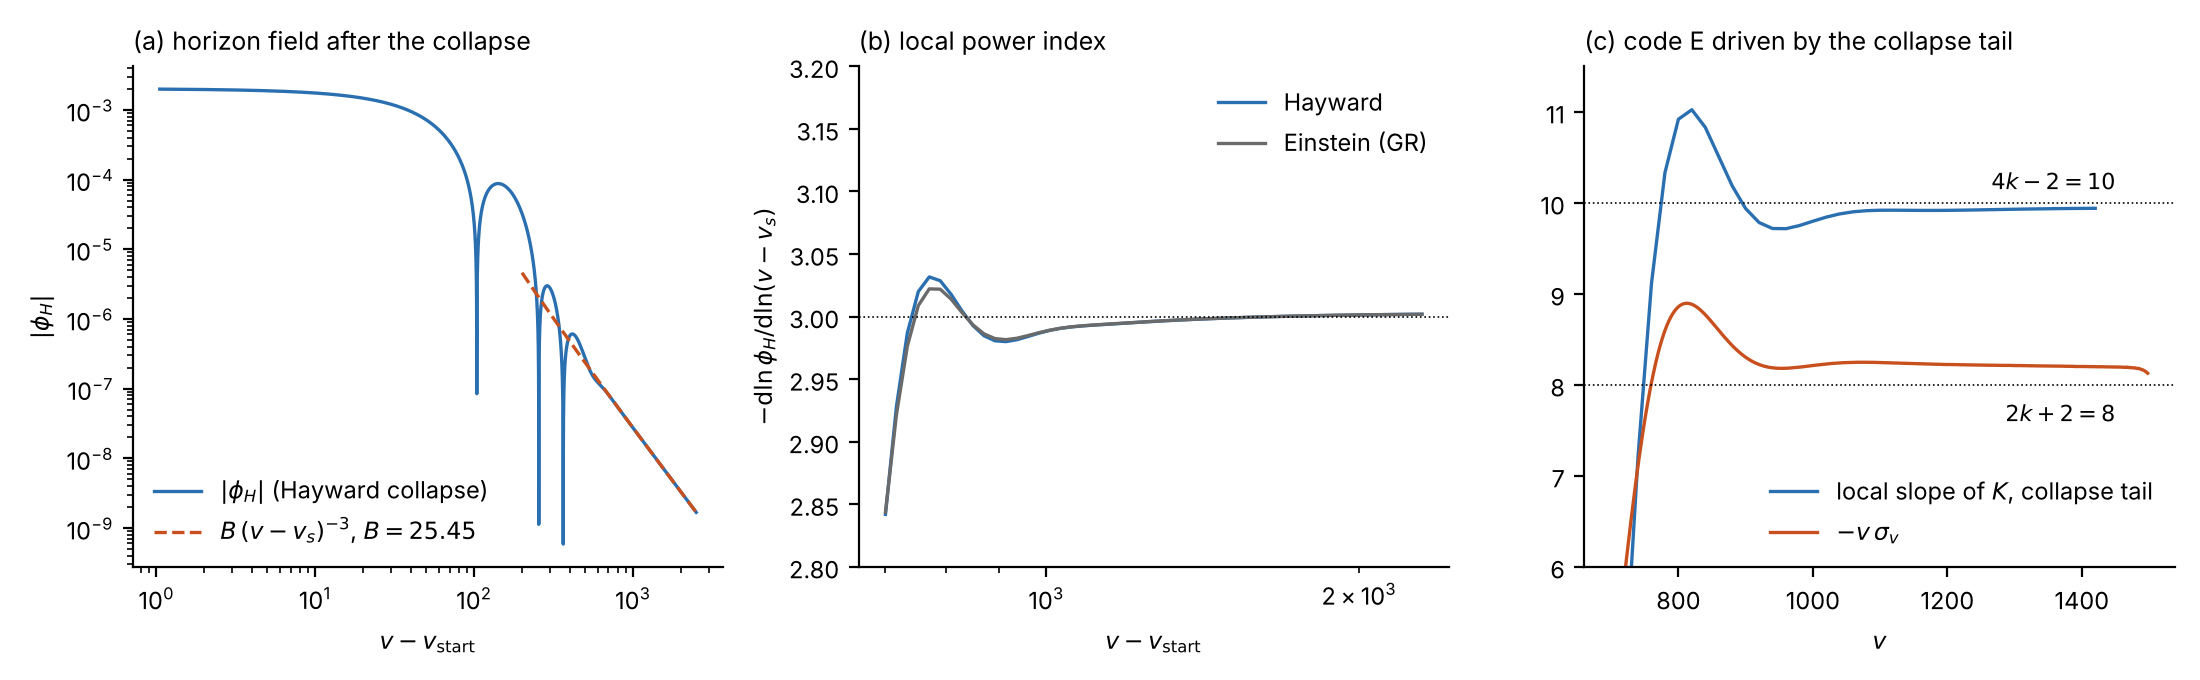
\includegraphics[width=\textwidth]{fig_collapse.png}
\caption{(a) Horizon field of the Hayward collapse ($m=5$, $\ell=1$) from the start of stage~L and the fit $B(v-v_s)^{-3}$. (b) Local power index of $\phi_H$ for the Hayward and Einstein cases. (c) Code~E driven by this table: local slope of $K$ and $-v\sigma_v$ on $U\simeq1$ against $4k-2=10$ and $2k+2=8$ ($k=3$).}
\label{fig:collapse}
\end{figure}

\paragraph{Code E on the collapse tail.} The table $\phi_H(v)$ ($v=0$ at $v_{\rm start}$, spacing $0.1$, to $v=2500$) replaces $B(1+v)^{-k}$ in the horizon Raychaudhuri equation (backward shooting from $r_v=0$ at $v_1+300$, so the horizon column is the teleological one for this table), in $\phi_v^{H}$ and in the starting data; the static row of Section~\ref{sec:ehdata} is used unchanged, as the test (ii) above supports, and the field on it is the collapse profile $\mathrm d\phi/\mathrm dr$ of stage~N times the static $r_U$ (\texttt{PU0MODE=profile}) rather than $\phi_U=0$. All else is code~E (Section~\ref{sec:seed}, $h_s=0.2$, $h_v=0.2$, to $v_1=1500$, $\kappa_+v_1=73$; \texttt{genc\_*.json}). Results (ray $U=0.9968$; \texttt{collapse\_E.log}):
\begin{itemize}
\item the front arrives at $v\simeq53$--$78$ on the four rays (the first $v$ at which $1-\ell^{2}\psi$ has fallen to half its value at $v=45$), earlier than for the prescribed $B=3\times10^{-3}$, $k=3$ ($73$ on $U\simeq1$) because the quasi-normal ringing, $|\phi_H|\sim2\times10^{-3}$ at the start, is a larger and more rapidly varying flux than the tail;
\item behind the front, $zm=0.59117$ against the closed form $0.59126$ (and $0.59117$ for the prescribed $k=3$ run), $\mathrm dm/\mathrm dv=4.403$ in both, $m=5742$ at $v=1400$; $r=r_-$ to $10^{-5}$;
\item $-v\sigma_v=8.246$ at $v=1100$ and $8.20$ at $1400$, tending to $2k+2=8$ from above in modulus ($8.081$ at $1100$ for the prescribed run);
\item the local slope of $K$ is $9.915$ at $v=1100$ and $9.94$ at $1450$ on $U\simeq1$ ($9.83,\,9.90,\,9.94,\,9.95$ at $v=1400$ on the four rays), against $4k-2=10$ and $9.47$ for the prescribed run at $1100$; it overshoots to $11$ near $v=800$, when the oscillations of the field have died down (Fig.~\ref{fig:collapse}c);
\item the amplitude of $K$ is not universal: $K(1400)=1.3\times10^{33}\ell^{-4}$ on $U\simeq1$, and with $\phi_U=0$ on the starting row $1.3\times10^{31}$ (factors $2.6,\,8.3,\,99,\,6\times10^{4}$ on the four rays at $v=1100$), while $\phi_v$ agrees to $4\times10^{-6}$, $\sigma_v$ to three digits and $m$, $z$ to $0.6\%$ (the field $\phi_U$ on a fixed ray differs by the factors $0.76,\,0.53,\,0.13,\,-0.13$ on the four rays, which enters $K$ through $g=\phi_U\phi_v/W$); the exponents are the same. $K$ at fixed late $v$ decreases with the tail amplitude in the prescribed runs ($K(1000)=5\times10^{37},\,5\times10^{29},\,5\times10^{21}$ for $B=3\times10^{-4},\,3\times10^{-3},\,3\times10^{-2}$, $k=\tfrac32$), so no ordering with the collapse amplitude should be read into the values.
\end{itemize}
\emph{Mesh dependence} ($h_v=0.2\to0.1$, $h_s=0.2$; \texttt{conv\_c.log}): the change is $4.3\times10^{-6}$ in $r$ (relative), $8\times10^{-6}$ in $\sigma_v$ (absolute; $1.1\times10^{-5}$ at $v=100$ on the first ray) and in $\phi_v$ (relative), $(1$--$4)\times10^{-5}$ in $\ln m$ (at most $3.6\times10^{-5}$) and $\le7.1\times10^{-4}$ in $\ln K$ at $v=100$, decreasing to $\le1.2\times10^{-4}$ at $v=1400$, on all four rays; $-v\sigma_v=8.19$ at $v=1400$ for $h_v=0.1$ ($8.20$ for $0.2$).

\paragraph{The other exponent: data with a nonzero Newman--Penrose constant.} \emph{What the literature fixes.} For $\ell=0$ on a static, asymptotically flat, spherically symmetric exterior, \citet{AngelopoulosAretakisGajic2018} prove that if the Newman--Penrose constant $I_0=\lim_{r\to\infty}r^{2}\partial_r(r\phi)$ (with $\partial_r$ at fixed $u$; it is the same on every outgoing cone) does not vanish, then $\phi\sim4I_0\,\tau^{-2}$ on and outside the horizon ($\tau=v$ on $\mathcal H^{+}$), with a coefficient that does not contain $m$, while for compactly supported data the leading term is $-8I_0^{(1)}\tau^{-3}$, $I_0^{(1)}$ being the constant of the time integral of the field. These are the two exponents of Price's law, $k=2$ for initially static and $k=3$ for generic compact data \citep{Price1972,GundlachPricePullin1994}; \citet{GundlachPricePullin1994b} found them in nonlinear collapse at fixed $r$ ($-2.08\ldots-1.86$ for static data against $-2$, $-2.74\ldots-2.63$ for Gaussian data against $-3$), and momentarily stationary compact data fall faster, as $t^{-4}$ \citep{KarkowskiSwierczynskiMalec2004,PriceBurko2004}. For the wave equation on a \emph{given} dynamical black-hole exterior that settles to Schwarzschild, \citet{GajicKehrberger2025} write the leading coefficient of the compact-data tail as a time-inverted Newman--Penrose constant with a part fixed by the initial data and a part that is an integral over the horizon (through the expansion of its generators) and over null infinity (through the integral of the Bondi news, whose spherical average is the Bondi mass); this is the structure that Eqs.~\eqref{eq:qabs} and~\eqref{eq:Fabs} below make explicit in spherical symmetry for strong data (initial-data charge $Q_0$ and horizon term $Q_{\rm abs}$). Their metric is an assumption and is not required to solve the Einstein equations. For the self-gravitating scalar they refer to \citet{Gautam2024}, who proves, for the spherically symmetric Einstein--Maxwell--scalar system, for smooth compactly supported data that settle to a subextremal Reissner--Nordstr\"om hole ($0<|e|<M$) and without smallness, that $\varphi$ on the event horizon is $C_0\,\mathfrak L[\varphi]\,v^{-3}+O(v^{-3-\delta})$ with an explicit non-zero $C_0$ and a dynamical constant $\mathfrak L[\varphi]$ that is non-zero exactly for the generic class of data of Luk and Oh (as read, the constant is not given in terms of the data, and the uncharged case is not stated separately). We did not find a published horizon coefficient for self-gravitating collapse data with a nonzero Newman--Penrose constant; the theorem of \citet{AngelopoulosAretakisGajic2018} is for the linear field on a fixed stationary background, and the question here is whether the strong-field collapse leaves it unchanged. \emph{Data.} To the pulse on $u=u_0$ we add, as a function of the areal radius along the ray, $\phi_{\rm tail}=b\,S\bigl((r-r_a)/\Delta r\bigr)/r^{2}$, $S(x)=x^{4}(35-84x+70x^{2}-20x^{3})$ (a $C^{3}$ ramp), $r_a=25.3$, $\Delta r=1.8$ (it ends at $r=27.1<r(u_0,v_1)=27.51$): $\phi_v=\phi_{\rm tail}'(r)\,r_v$ enters the ray equations of stage~N, $r\phi=b/r$ for $r\ge r_a+\Delta r$, and $I_0=-b$ exactly, the other data being those above ($A$ is retuned to $m=5$: $A=0.030015$ and $m_f=4.99982$ at $(u_0,v_1)$ for $b=1$; the tail carries $1.8\times10^{-4}$ of mass beyond $v_1$, which is not in the static background of stage~L). In stage~L the same $\psi=b\,S/r$ is the datum on $u_e=u_{e0}$, $v>v_1$, with $r(r_*)$ of the static exterior, and the row of stage~N carries the constant $\phi(u_0,v_1)=b/r^{2}$ in $\phi=\phi(u_0,v_1)+\int\phi_u\,\mathrm du$ (it is zero for the compact pulse).

\emph{Tests.} (a) \emph{Stage~L alone}: $\psi=0$ on the row, the tail on the ray, the static $m=5$ exterior of Schwarzschild or Hayward, $h_L=0.2$, to $t=12800$ (\texttt{nplin.log}). $\phi_H\,t^{2}/(-4b)=0.9295,\,0.9649,\,0.9826,\,0.9914$ at $t=800,\,1600,\,3200,\,6400$ ($t=v-v_{\rm start}$); fitting $a_0[1+(c_1+c_2\ln t)/t+(c_3+c_4\ln t)/t^{2}]$ on $t\ge800$, $1600$, $3200$ gives $a_0=1.0000\pm0.0002$ (to $4\times10^{-5}$ with the full form), the same for the two backgrounds to $10^{-4}$, and a free fit $k=2.0005$: the coefficient of the theorem, $4I_0$ with no free parameter, is reproduced, including the $\ln t/t$ correction. (b) \emph{Nonlinear collapse} (stage~N to $v_1=60$, $h_N=h_L=0.1$, to $t=12800$; \texttt{np\_fit.log}): the same fits give $a_0=1.0000$ for $b=1$ (Hayward and Einstein), $-1$, $0.5$, $2$ ($|a_0-1|\le3\times10^{-5}$ for the full form and $t\ge1600$, $\le1.5\times10^{-4}$ with only the $c_1/t$ correction), and the free fit gives $k=2.0013,\,2.0007,\,2.0004$ for windows starting at $t=800,\,1600,\,3200$ with $B/(4|b|)=1.013,\,1.007,\,1.004$ (fitted shift $s\simeq-44$ in $B(t-s)^{-k}$, which is why $B$ at a given window differs from $4|b|$: the leading coefficient is $a_0$). The collapse changes the transient and the subleading terms (Fig.~\ref{fig:k2}a: for $t\lesssim700$ the curves differ, with minima $0.29$ and $0.52$ of the limit for the collapse and the linear test, and they merge afterwards) and not the limit. The response is linear in the amplitude of the tail: $[\phi_H(b)-\phi_H(0)]/b$ for $b=0.5,\,1,\,-1,\,2$ (the pulse is retuned to $m=5$ each time) differs by a relative $8\times10^{-3}$ at $t=50$, $10^{-4}$ at $100$, $6.5\times10^{-4}$ at $200$ and $\le6\times10^{-5}$ for $t\ge400$ (\texttt{np\_lin\_b.log}). (c) \emph{Matching}: stage~N to $v=150$ against stage~L from $v=70$ (Einstein, $b=1$) agrees to $10^{-3}$ at $r_*=35$, $1.3\times10^{-4}$ at $20$ and $1.1\times10^{-4}$ at $-9$ (\texttt{overlap\_np.log}; $4\times10^{-5}$, $2.5\times10^{-4}$ and $1.6\times10^{-2}$ for the compact pulse). Thus the index is $2$ and the coefficient is $4I_0$ in the collapse, in both models: the strong-field stage does not change the leading coefficient, which is fixed by the data at large radius. The collapse does not enter that coefficient, in contrast with the compact case below.

\emph{Data with a nonzero scalar charge at infinity ($r\phi\to\psi_\infty\neq0$).} The datum above has $r\phi\to0$ at infinity. The initially static case of the literature has instead a field that is the static solution of the wave equation outside a radius: on the static background of mass $m$ the solution regular at infinity obeys $r^{2}f\,\partial_r\phi=$ const, $g(r)=\int_0^{1/r}\mathrm ds/f(1/s)=1/r+m/r^{2}+O(r^{-3})$ (for the Hayward $f$ too, since $f=1-2m/r+O(r^{-4})$), so that $r\phi\to\psi_\infty=c$ and $I_0=-c\,m$ for $\phi=c\,g(r)$. We use $\phi_{\rm tail}=c\,S\bigl((r-r_a)/\Delta r\bigr)g(r)$ on $u=u_0$ ($g$ for the target mass $m_t$ and the model run; a spline of the quadrature, checked against $g\,r\to1$ and $(g-1/r)r^{2}/m\to1$), with $c=0.02$, the ramp of the previous datum and the same stage~N/stage~L pipeline; in stage~L the same profile is the datum on the ray and the row carries $\phi(u_0,v_1)=c\,g(r(u_0,v_1))$ (\texttt{collapse\_lib.py:np\_tail}, \texttt{strong\_table.py} with \texttt{TAIL\_C}). The tail carries a mass of order $c^{2}$ beyond $v_1$ that the static background of stage~L does not contain ($m_f=4.99962,\,4.99849,\,4.99397$ for $c=0.01,\,0.02,\,0.04$ against $5$: deficits $3.8,\,15.1,\,60.3\times10^{-4}$, i.e.\ $\propto c^{2}$); the prediction below uses $m_t=5$. Result (collapse of the pulse from flat space, $m_0=0\to m_t=5$, $h_N=h_L=0.1$, $t\le12700$; \texttt{tc\_fit.py}, \texttt{tc\_fit.log}): the horizon field is $\phi_H=a_0\cdot4I_0\,t^{-2}[1+\ldots]$ with $a_0=0.99993$ (Hayward, $c=0.02$, window $t\ge800$, full form), $0.99993$ (Einstein), $0.99999$ ($t\ge1600$) and $1.0000$ ($t\ge3200$) for both; for the Hayward model at $c=0.01$ and $0.04$ $a_0=0.99999$ and $0.99990$ ($t\ge800$), $1.0000$ and $0.99999$ ($t\ge3200$); for a pulse collapsing into an existing hole ($m_0=2.5\to5$) $0.99992$, $0.99999$; for a hole of twice the mass ($m_0=0\to10$, $t\le25400$, windows scaled by $2$) $1.0000$ at $t\ge3200$ (the window $t\ge800$ is too early on that scale: $1.0045$). Free-index fits $\phi_H=B(t-s)^{-k}$ give $k=2.0020,\,2.0010,\,2.0005$ for $t\ge800,\,1600,\,3200$ ($c=0.02$, Hayward and Einstein alike) with $B/(4|I_0|)=1.020,\,1.010,\,1.005$ (the offset $s$ again), and $2.0004$--$2.0010$ for the other cases at $t\ge3200$ ($2.0021$ for $m_t=10$). Thus, to $10^{-4}$, the horizon field of the strong collapse of data with $\psi_\infty\ne0$ is the linear-theory value $4I_0t^{-2}$ with $I_0=-c\,m$: it is linear in $c$ (a factor $4$ in $c$, $16$ in the mass defect, leaves $a_0$ unchanged to $10^{-4}$), the same in Einstein gravity and in the Hayward model, and independent of $m_0$ and of the scale of $m$. The constant $I_0=-c\,m_t$ is a property of the data ($g$ is built with $m_t$), and the data prefer it to $-c\,m_f$ ($a_0=0.99999$ against $1.0012$ at $c=0.04$, $t\ge3200$): the mass of order $c^{2}$ that the tail carries beyond $v_1$ does not enter the coefficient.

\emph{Code E on the $k=2$ tail} ($b=1$ and $0.1$; $\phi_H$ table to $v=2500$ with $h_N=0.05$, $h_L=0.1$, $v_1=60$; $h_s=h_v=0.2$ to $v_1=1500$; \texttt{collapse\_E\_k2.log}). The starting row is the static one of Section~\ref{sec:ehdata} (the interior stays at $m=5.0011$ and $r=r_-=1.05746$ up to the front, as it must; a row without the constant $\phi(u_0,v_1)$ puts $m\simeq5.4$ there and $r=1.0526$, and was discarded). Behind the front ($v_{\rm front}=53,\,80,\,67,\,61$ on the four rays for $b=1$): $zm=0.59114$--$0.59119$ ($\tfrac12r_-^{3}=0.59126$), $\mathrm dm/\mathrm dv=4.42$ at $v=1400$ for both amplitudes (closed form $4.449$; $4.41$ for $k=3$), i.e.\ independent of $k$ and $b$ as in Section~\ref{sec:curv3}; $v\sigma_v=-5.800,\,-5.839,\,-5.867$ at $v=1000,\,1200,\,1400$ ($b=1$) and $-5.507,\,-5.612,\,-5.685$ ($b=0.1$), tending to $-(2k+2)=-6$ from below; the local slope of $K$ is $5.07,\,5.23,\,5.34$ ($b=1$) and $4.37,\,4.68,\,4.90$ ($b=0.1$) at the same $v$, still $11\%$ and $18\%$ below $4k-2=6$, and with the two $1/v$ terms of Eq.~\eqref{eq:kslope} added back, with the measured $v_0$ ($81$ and $96$) and $v\sigma_v$, it is $5.998,\,5.993,\,5.987$ and $5.995,\,5.991,\,5.986$ on $U\simeq1$, and $5.99$--$6.00$ on the other three rays (Fig.~\ref{fig:k2}c): $K\propto v^{4k-2}$ with $k=2$ holds in the sense of Section~\ref{sec:curv3}, with $v_0$ delaying the approach more for the weaker tail. The fit $a+c/v$ to the slope of $b=1$ for $1000\le v\le1450$ gives $a=6.01$ ($c=-937$). $K$ at $v=1400$ is $4.5\times10^{21}$ ($b=1$) and $1.4\times10^{32}\ell^{-4}$ ($b=0.1$) on $U\simeq1$ (and $1.3\times10^{33}$ for the $k=3$ collapse tail), another sign that the amplitude of $K$ is not universal. Mesh ($h_v=0.2\to0.1$, $b=1$; \texttt{conv\_c\_k2.log}): $\le7.6\times10^{-4}$ in $\ln K$ at $v=100$, $\le4\times10^{-4}$ at $200\le v\le400$ and $\le1.5\times10^{-4}$ at $v\ge800$, $1.3\times10^{-5}$ in $\sigma_v$, $4.3\times10^{-6}$ in $r$, $5\times10^{-5}$ in $\ln m$ and $9\times10^{-6}$ in $\phi_v$, on all four rays.

\begin{figure}[t]
\centering
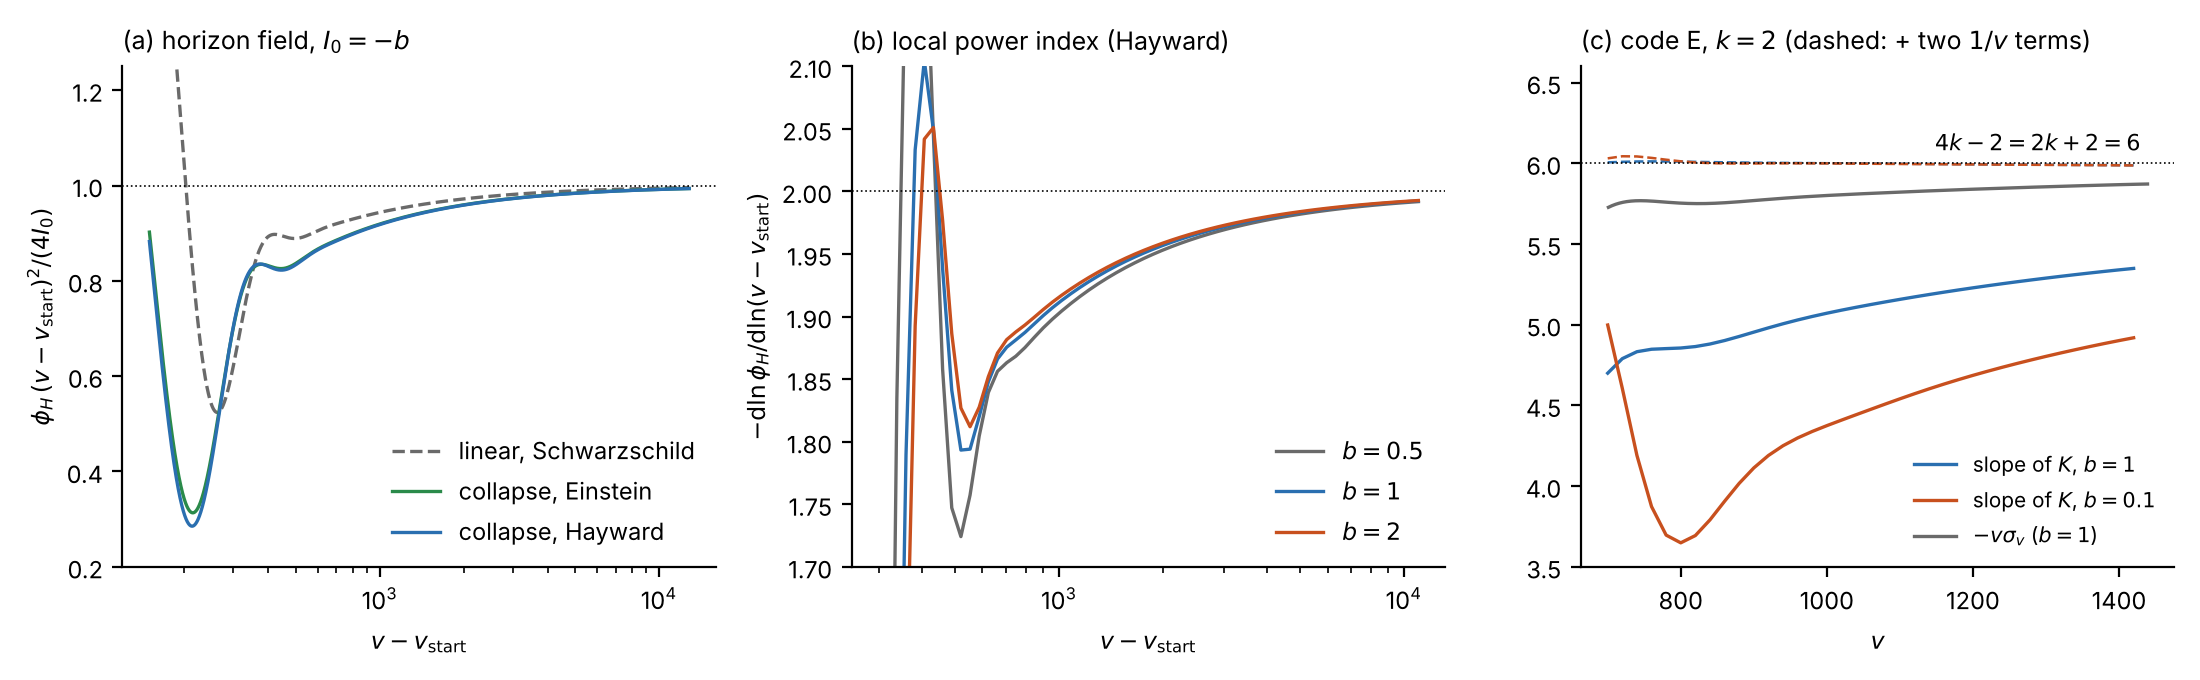
\includegraphics[width=\textwidth]{fig_collapse_k2.png}
\caption{Collapse data with a nonzero Newman--Penrose constant ($I_0=-b$). (a) $\phi_H t^{2}/(4I_0)$ for the linear problem on Schwarzschild and for the Einstein and Hayward collapses ($m=5$, $b=1$): the coefficient tends to $1$. (b) Local index of $\phi_H$ for the Hayward collapse, $b=0.5,\,1,\,2$. (c) Code~E driven by the $k=2$ tables: local slope of $K$ (solid) and with the two $1/v$ terms added back (dashed) for $b=1$, $0.1$, and $-v\sigma_v$ ($b=1$), against $4k-2=2k+2=6$.}\label{fig:k2}
\end{figure}

\emph{The coefficient for compact data.} The field equation implies the exact conservation law $\partial_u(r^{2}\phi_v)+\partial_v(r^{2}\phi_u)=0$ (the Noether current of $\phi\to\phi+c$), so $Q=\int r^{2}\,\mathrm d\phi$ along the ray $u=u_0$ is a property of the data, in the linear and nonlinear problems alike. In the linear problem (pulse on the ray, $\psi=0$ on the row, static background) the fitted coefficient of the $v^{-3}$ tail is $B_{\rm lin}=68.24,\,38.38,\,103.9$ for the three amplitudes $A/A_0=1,\,0.8,\,1.2$ ($m=5,\,3.21,\,7.18$), and $8m|Q|=68.24,\,38.38,\,103.9$ ($|Q|=1.706,\,1.495,\,1.810$): ratio $1.0000\pm10^{-4}$ for the first two, $1.001$ for the third (the windows start at $t\ge1600$; \texttt{linear\_q.log}), and the same for Schwarzschild and Hayward, so that $I_0^{(1)}=+mQ$ in the notation of \citet{AngelopoulosAretakisGajic2018} for this class of data ($Q<0$ for the positive pulses used here, so $I_0^{(1)}<0$ and $B=-8I_0^{(1)}=8m|Q|$) (for the Schwarzschild exterior the integral expression of this constant is Eq.~(1.5) of \citet{GajicKehrberger2025} with $g=g_M$, which gives $I_0=\tfrac12MQ$ in their normalization and hence $B=8M|Q|$, see the discussion of that theorem below; for the Hayward exterior the constant is identified numerically; $Q=0$ for momentarily stationary data, which fall as $t^{-4}$, is consistent). In the collapse the measured coefficient is $B/(8m|Q|)=0.430,\,0.403,\,0.373,\,0.336,\,0.294$ for $A/A_0=0.8,\,0.9,\,1,\,1.1,\,1.2$ (\texttt{ascale\_q.log}: $0.4302,\,0.4026,\,0.3727,\,0.3358,\,0.2944$; this is the $0.37$ of the linear estimate quoted above): $Q$ is the same, $m$ is that of the final hole, and the collapse removes a fraction of the tail that grows with the strength of the pulse; the charge on the exterior part of the row $v=60$ ($r>r_+(m)$; \texttt{ascale\_q.py}, \texttt{ascale\_q.log}) is $-0.27,\,-0.37,\,-0.43,\,-0.39,\,-0.33$ and does not reproduce $B$ either ($B/(8m|Q_{\rm row}|)=2.4,\,1.8,\,1.5,\,1.5,\,1.6$). So the $v^{-3}$ coefficient of a collapse is a functional of the nonlinear history, which we have not derived, while the $v^{-2}$ one is a property of the data at infinity.

\paragraph{Strength of the infalling pulse and the inner radius.} \citet{ShaoGuoTianZhang2025} evolve a scalar field on the Hayward geometry sourced by non-linear electrodynamics in general relativity and report that a strong enough field shrinks the inner horizon to zero (we use their abstract; their threshold is a statement about a different theory). The analog in the present theory is a test of whether the inner radius depends on the strength of what falls in. \emph{Static bound.} $r_-(m)$ is the smallest positive root of $g(r)=r^{3}-2mr^{2}+2m$ ($\ell=1$); $g(0)=2m$, $g(1)=1$ and $g'(r)=r(3r-4m)<0$ on $(0,4m/3)$, so $g>0$ on $(0,1]$ and $r_->\ell$ for every $m$ with horizons, with $r_-\to\ell$ only as $m\to\infty$ ($r_-=1.0575,\,1.0267$ for $m=5,\,10$). A threshold at which $r_-\to0$ is therefore not available to a Hayward hole of this theory by the choice of its mass, and the question is whether the dynamics can do it. \emph{Data.} To the horizon table of the $k=3$ collapse of this section (Hayward, $m=5$) we add a prescribed pulse $P\sin^{4}\bigl(\pi(v-10)/20\bigr)$ on $10\le v\le30$ ($\phi_H$ is event-horizon data as in Section~\ref{sec:curv3}; this pulse is not generated by a collapse), and run code~E on the starting row of $m=5$ ($h_s=h_v=0.2$, $v\le1000$, \texttt{codec/sc/}). The horizon column is the event horizon: backward shooting of the horizon Raychaudhuri equation from $v=1300$ ($=v_1+300$) with $r_v=0$ there, for the final radius $r_f$ for which $r(0)=r_+(5)$ (the same $r_f$ to $10^{-4}$ when the shooting starts at $v=310$), and $m_f$ is the mass of the static hole with $r_+(m_f)=r_f$. The root exists on a monotone branch for $P\le0.08$. For $P=0.09$ the map $r_f\mapsto r(0)$ has a maximum of $9.19<r_+(5)=9.90$ near $r_f=30$ (a fold) and returns to $r_+(5)$ only at $r_f\simeq145$ ($m_f\sim70$, a branch we do not follow); at $P=0.1$ the local maximum is $5.1$ (\texttt{horizon\_map.log}). This is a property of prescribing the field on the horizon: a Vaidya-like estimate $\mathrm dm/\mathrm dv=4\pi r_+(m)^{2}\phi_v^{2}$ (not exact: it overestimates $m_f$ by $0.3\%$ at $P=0.01$ and $18\%$ at $0.08$, and the Einstein version does the same) has a pole at a finite strength, between $P=0.10$ ($m_f=21.6$) and $0.12$, because the horizon area grows with the mass (\texttt{vaidya\_estimate.log}), so a field profile fixed on the horizon cannot be scaled up indefinitely on a starting row of mass $5$. The scan ends at $P=0.08$ (a horizon mass gain of $3.3$ on $m=5$).

\begin{table}[ht]\centering\small
\begin{tabular}{rrrrrrrrr}
\hline
$P$ & $r_f$ & $m_f$ & $r_\infty$ & $m^{*}$ & $m_{\rm ray}$ & $r_-(m_f)$ & $\mathrm dm/\mathrm dv$ & asympt.\\
\hline
0.01 & 9.946 & 5.024 & 1.05711 & 5.028 & 5.029 & 1.05716 & 4.41 & 4.48\\
0.03 & 10.354 & 5.226 & 1.05436 & 5.248 & 5.260 & 1.05462 & 4.61 & 4.70\\
0.05 & 11.357 & 5.723 & 1.04903 & 5.746 & 5.752 & 1.04925 & 5.11 & 5.20\\
0.07 & 13.723 & 6.898 & 1.03985 & 6.915 & 6.916 & 1.03996 & 6.33 & 6.38\\
0.08 & 16.597 & 8.329 & 1.03223 & 8.396 & 8.396 & 1.03251 & 7.82 & 7.87\\
\hline
\end{tabular}
\caption{Pulse-strength scan of code~E ($m=5$ start, ray $U\simeq1$). $r_f$: final radius of the event horizon; $m_f$: mass with $r_+(m_f)=r_f$; $r_\infty$: radius of the ray at $v\ge200$ (constant to $2\times10^{-6}$ after the front); $m^{*}$: the mass with $r_-(m^{*})=r_\infty$; $m_{\rm ray}$: $r^{3}\psi/(2z)$ on the ray at the first $v$ with $|r-r_\infty|<3\times10^{-5}r_\infty$ ($v=42,\,45,\,50,\,64,\,84$), before inflation; $\mathrm dm/\mathrm dv$: the mean over $800\le v\le900$ against the closed form~\eqref{eq:dm} at $r_\infty$.}\label{tab:pscan}
\end{table}

\emph{Result} (Table~\ref{tab:pscan}; \texttt{scan\_summary.log}). The inner radius behind the front is $r_\infty=r_-(m_f)$ to $5\times10^{-5}$ at $P=0.01$ and to $(1$--$3)\times10^{-4}$ for the others; the mass $m^{*}$ implied by $r_\infty$ differs from $m_f$ by $0.1$--$0.8\%$, and from the ray mass just before inflation by $0.03\%$, $0.22\%$, $0.12\%$, $0.003\%$ and $<10^{-4}$ for the five strengths. The radius falls from $1.0571$ to $1.0322$ as the mass grows by $3.3$ and stays above $\ell$; $zm\to\tfrac12r_-^{3}$ in each run (\texttt{scan\_zm.log}) ($0.59055,\,0.58596,\,0.57713,\,0.56213,\,0.54987$ at $v=900$ against $0.59065,\,0.58605,\,0.57721,\,0.56219,\,0.54992$) and the rate $\mathrm dm/\mathrm dv$ follows the closed form~\eqref{eq:dm} evaluated at the new $r_-$, rising from $4.4$ to $7.8$ (the measured value is $0.7$--$1.8\%$ below it, which is of the size of the mesh dependence (below): the closed form is the limit $v\to\infty$, approached from below as in Section~\ref{sec:endpoint}). The late-time quantities that depend on the tail and not on the pulse do not: $v\sigma_v=-8.30,\,-8.31,\,-8.33,\,-8.38,\,-8.45$ and $\mathrm d\ln K/\mathrm d\ln v=10.02,\,10.03,\,10.02,\,9.94,\,9.83$ at $v=900$ (\texttt{scan\_an.log}; $-(2k+2)=-8$ and $4k-2=10$ for $k=3$, approached from below as in the single-amplitude runs). So within the range reached the pulse sets the mass and, through it, $r_-$, $\mathrm dm/\mathrm dv$ and the amplitude of $K$, and not the structure behind the front; the inner radius does not vanish at any strength reached, in line with the bound above. We do not see a threshold of the kind reported for the electrodynamic model; since the Hayward form here is a property of the gravitational theory and not of a matter background, and the data are restricted to be regular on the event horizon (for which $m$ can only grow, Proposition~\ref{prop:y}), this is a difference between the two systems and not a test of their result. \emph{Mesh.} Halving $h_v$ at $P=0.08$ ($h_s=0.2$; \texttt{conv\_P0.08\_hv.log}) changes, over the four rays, $r$ by $4.4\times10^{-5}$ ($r_\infty=1.03227$, so the difference from $r_-(m_f)$ is not a mesh effect), $\sigma_v$ by $4\times10^{-5}$ ($7\times10^{-4}$ at $v=100$), $\ln m$ by $9\times10^{-4}$ and $\ln K$ by $7\times10^{-3}$ for $v\ge400$ ($8.4\times10^{-3}$ at $v=200$, $2.2\times10^{-2}$ at $v=100$; the amplitude of $K$ is the least converged quantity, as the pulse is the strongest); $\mathrm dm/\mathrm dv=7.809$ against $7.816$, and the slope of $K$ at $v=900$ is $9.825$ in both. Halving $h_s$ at $P=0.07$ ($h_v=0.2$; \texttt{conv\_P0.07\_hs.log}) moves $r_\infty$ by $+5.3\times10^{-5}$ to $1.03991$ ($5\times10^{-5}$ from $r_-(m_f)$), $\sigma_v$ by $\le2.6\times10^{-4}$ ($\le1.2\times10^{-6}$ for $v\ge200$), $\ln m$ by $10^{-3}$--$4\times10^{-3}$, $\ln K$ by $6\times10^{-4}$--$1.4\times10^{-2}$ for $v\ge200$, $\mathrm dm/\mathrm dv$ from $6.334$ to $6.279$ ($0.9\%$, so the $0.7$--$1.8\%$ offset from the closed form is of the size of the mesh dependence) and the slope of $K$ at $v=900$ from $9.940$ to $9.973$. Not shown: pulses with $P>0.08$ (no such event-horizon column exists, see above), data that are not regular on the event horizon, a pulse that changes the starting row itself (the collapse-generated pulse is the next paragraph; here the row is the static one of $m=5$ and the pulse arrives at $v=10$, with the horizon column carrying the anticipation).

\paragraph{A strong pulse generated by collapse into an existing hole.} The scan above ends at a fold of the horizon column, which we attribute to prescribing $\phi$ on the horizon; the test is a pulse that is generated by the evolution. \emph{Data.} In stage~N the data on $v=v_0$ are now those of a static hole of mass $m_0$ and the data on $u=u_0$ carry the pulse as before. In the gauge $\sigma=0$ on both rays the static solution has $r_u=-\tfrac12$, $r_v=\tfrac12f(r)$ and $\sigma_v=\tfrac12\bigl(f'(r)-f'(r_c)\bigr)$ along $v=v_0$ ($r=r_c-u/2$, $r_c=(v_0-u_0)/2$), and $r_v=\tfrac12f(r_c)$ before the pulse and $\sigma_u=0$ at the corner along $u=u_0$ ($f=1-2m_0r^{2}/(r^{3}+2m_0\ell^{2})$; $f'=rQ(\psi)$ makes the ray equation $\partial_vr_u=-\tfrac14rQ$ consistent with the static data); $m_0=0$ is the flat start used so far (\texttt{collapse\_lib.rays(..., m0=)}). The geometry is scaled with $s=\max(1,m_f/5)$ ($r_c=20s$, pulse on $v_0+[4,12]s$, $v_1=v_0+20s$, $h_N=0.1s$, $h_L=0.1s$), the data on $v_0$ stop at $r_+(m_0)+0.1$ (deeper cells of the old interior are amplified as $e^{\kappa_-v}$ and are not needed: the dependence is on smaller $u$ only), and $A$ is tuned so that the generalized mass on $u_0$ after the pulse is $m_f$ (\texttt{strong.py}, \texttt{strong\_table.py}; stage~L with the static exterior of $m_f$ as before). \emph{Tests.} (i) $A=0$, $m_0=5$: the row $v_1=60$ stays the static hole, $\max|m-m_0|=7.1\times10^{-4},\,1.8\times10^{-4},\,4.5\times10^{-5}$ for $h=0.2,\,0.1,\,0.05$ (ratio $4.0$; \texttt{t\_static\_h.py}). (ii) $m_0=0$ reproduces the earlier table ($A=0.030030$, $v_{1e}$ to $10^{-12}$, $\phi_H$ to $3.8\times10^{-5}$ of its maximum). (iii) After a pulse that raises $m_0=5$ to $m_f=10$ or $25$ the row $v_1$ is the static hole of $m_f$: $\max|\psi/\psi_s-1|=3\times10^{-6}$ ($7\times10^{-6}$ at $0.05s$) for $r>1.5r_+$ and $\le4\times10^{-5}$ down to $0.9r_+$ for $m_f=10$ ($2.5\times10^{-5}$ for $m_f=25$), at $h_N=0.1s$ (the bounds $4\times10^{-5}$ and $2.5\times10^{-5}$ hold at $0.05s$ as well) (\texttt{sp\_interior.py}); halving $h_N$ or $h_L$ changes $\phi_H$ by $\le3.5\times10^{-5}$ and $1.5\times10^{-6}$ of its maximum (\texttt{strong\_conv.py}), and stage~N to $v_1+80s$ against stage~L from $v_1$ agrees to $4\times10^{-5},\,3\times10^{-5},\,9\times10^{-5}$ at $r_*=69,\,41,\,12$ ($m_f=10$; \texttt{overlap\_h.py}).

\begin{table}[ht]\centering\small
\begin{tabular}{rrrrrrr}
\hline
$m_0$ & $m_f$ & $A$ & $|Q|$ & $B$ & $B/(8m_f|Q|)$ & $B/m_f^{3}$\\
\hline
5 & 5.01 & 0.00140 & 0.0464 & 1.87 & 1.004 & 0.0148\\
5 & 5.5 & 0.00939 & 0.398 & 16.30 & 0.930 & 0.0980\\
5 & 6.5 & 0.01487 & 0.960 & 41.15 & 0.824 & 0.1498\\
5 & 8 & 0.01885 & 2.004 & 92.94 & 0.725 & 0.1815\\
0 & 10 & 0.03003 & 6.824 & 202.68 & 0.371 & 0.2027\\
2.5 & 10 & 0.02626 & 5.309 & 212.96 & 0.501 & 0.2130\\
5 & 10 & 0.02165 & 3.853 & 198.88 & 0.645 & 0.1989\\
7.5 & 15 & 0.02165 & 8.669 & 670.85 & 0.645 & 0.1988\\
10 & 20 & 0.02165 & 15.41 & 1589.9 & 0.645 & 0.1987\\
5 & 15 & 0.02484 & 10.84 & 711.88 & 0.547 & 0.2109\\
5 & 20 & 0.02626 & 21.23 & 1702.0 & 0.501 & 0.2127\\
2.5 & 12.5 & 0.02707 & 8.759 & 415.42 & 0.474 & 0.2127\\
5 & 25 & 0.02707 & 35.04 & 3321.3 & 0.474 & 0.2126\\
\hline
\end{tabular}
\caption{Tail of a pulse generated by collapse into a hole of mass $m_0$ (Hayward, $h_N=h_L=0.1s$, $B$ from $\phi_H=B(v_e-v_s)^{-3}$ on $[1000,2900]\,m_f/5$, fixed index; $|Q|=|\int r^{2}\phi_v\,\mathrm dv|$ along $u_0$). The free index is $3.011$--$3.012$ in every row.}\label{tab:strong}
\end{table}

\emph{Tail.} For $m_0=5$ the horizon field is again $B(v-v_s)^{-3}$ (free index $3.011$--$3.012$ in all rows, the offset of the $3.009$ of the flat start). For a weak pulse ($m_f=5.01$) $B/(8m_f|Q|)=1.004$: the linear identity $B=8m|Q|$ of Section~\ref{sec:collapse}, here reproduced by the nonlinear pipeline with the hole already present (the rest of the $0.4\%$ is the fit). For a strong pulse $F\equiv B/(8m_f|Q|)$ falls, and depends only on $\mu=m_0/m_f$: $0.645$ for $\mu=\tfrac12$ ($m_f=10,\,15,\,20$ from $m_0=5,\,7.5,\,10$), $0.501$ and $0.474$ for $\mu=\tfrac14$ and $\tfrac15$ (two scales each, agreement $\le10^{-3}$), $A$ and $|Q|/m_f^{2}$ being equal for equal $\mu$ (Fig.~\ref{fig:strong}a); the same table in Einstein gravity differs by $\le0.25\%$ ($B/m_f^{3}=0.1985,\,0.2125,\,0.2124,\,0.2022$ for $(m_0,m_f)=(5,10),\,(2.5,10),\,(5,25),\,(0,10)$ against $0.1989,\,0.2130,\,0.2126,\,0.2027$): at $m_f\ge10$ the exterior is that of general relativity, in which the problem has no scale. $F(\mu)$ is $0.371$ at $\mu=0$ (the flat start of the previous sections, where $0.373$ at $m_f=5$), and it satisfies $F\simeq\mu+0.23(1-\mu)$ near $\mu=1$ and $F-\mu=0.29(1-\mu)$ at $\mu=\tfrac12$, i.e.\ $B$ is $8|Q_0|$ times $m_0$ plus a fraction $0.23$--$0.37$ of the mass that the pulse brings. $B/m_f^{3}$ has a flat maximum $0.213$ at $\mu\simeq0.2$--$0.25$ and then falls to $0.2027$ at $\mu=0$ and to $0$ at $\mu=1$. The next paragraph explains the reduction; the dependence on the pulse width at fixed $\mu$ is not a function of $\mu$ alone ($F=0.363,\,0.370,\,0.384$ at $\mu=0$ and $0.632,\,0.644,\,0.668$ at $\mu=\tfrac12$ for pulses of width $4s,\,8s,\,16s$ with the same final mass, in Einstein gravity: the $8s$ values are $0.3704$ and $0.6441$, against $0.3713$ and $0.6451$ for the Hayward $h$), so the scale law above is for the pulse shape of Table~\ref{tab:strong}.

\emph{Why $F<1$: the charge absorbed by the growing horizon.} The scalar equation $\phi_{uv}+(r_u\phi_v+r_v\phi_u)/r=0$ is the same in all the models (the QTG corrections enter only the geometry); it is the conservation law of the Noether current of $\phi\to\phi+c$: $\omega=r^{2}\phi_v\,\mathrm dv-r^{2}\phi_u\,\mathrm du$ is closed, and on a null ray where $\phi$ vanishes at both ends the charge is $\int r^{2}\phi_v\,\mathrm dv=-\int\phi\,\mathrm d(r^{2})$. The charge $Q_0$ on $u_0$ is therefore the sum of the charge $Q_S$ on the row $v_1$ outside the event horizon and the charge $Q_H=\int_{\mathcal H}r^{2}\phi_v\,\mathrm dv$ through the event horizon between $v_0$ and $v_1$. In the linear problem on a fixed hole $r_H$ is constant, $Q_H=r_+^{2}[\phi_H]\to0$, nothing is absorbed in the end and the identity $B=8m|Q|$ of Section~\ref{sec:collapse} holds with the charge $Q_0$ of the data. In the nonlinear collapse the horizon grows and takes up a net charge
\begin{equation}Q_{\rm abs}=-\int_{\mathcal H}\phi\,\mathrm d(r^{2})=-\int 2\,r_H\dot r_H\,\phi_H\,\mathrm dv,\qquad Q_\infty=Q_0-Q_{\rm abs},\label{eq:qabs}\end{equation}
(after $v_1$ the exterior is the static hole of mass $m_f$ and $r_H$ is constant, so only $v<v_1$ contributes), and what remains outside, $Q_\infty=Q_S+r_+^{2}\phi_H(v_1)$ (the row charge plus the charge that the static horizon still takes after $v_1$, $-r_+^{2}\phi_H(v_1)$, with the opposite sign), is the charge that sources the tail in the final static exterior. Applying the linear identity there, $B=8m_f|Q_\infty|$, i.e.
\begin{equation}F=\frac{B}{8m_f|Q_0|}=1-\frac{Q_{\rm abs}}{Q_0}.\label{eq:Fabs}\end{equation}
The identity for data given on a slice follows from the time integral $\phi^{(1)}$ of the field ($\partial_t\phi^{(1)}=\phi$, regular at the horizon): in the static exterior $r^{2}f\,\partial_r\phi^{(1)}=Q(r)$, the charge inside $r$, so $\phi^{(1)}=-Q/r-mQ/r^{2}+\dots$ outside the support and $r^{2}\partial_r(r\phi^{(1)})\to mQ$, the Newman--Penrose constant of $\phi^{(1)}$, which is the quantity that fixes the $v^{-3}$ tail (this is the sketch of the slice form; its numerical content is the identification $I_0^{(1)}=+mQ$ of Section~\ref{sec:collapse}). \emph{Relation to the theorem of Gajic and Kehrberger.} The time-inverted Newman--Penrose constant of \citet{GajicKehrberger2025} is defined for $\Box_g\phi=F$ on a given dynamical exterior $g$ that settles to Schwarzschild $g_M$; the metric is not required to solve the Einstein equations. We have read the statements of their Theorems~1.1 and~4.1 and of Assumptions~3.1, 4.1 and~4.2, with Sections~2 and~3, and, for $\ell=0$ on Schwarzschild, the derivation of the constant (Proposition~7.1, Lemma~7.2); not the energy estimates of Section~5 or the iteration of Sections~7.4--7.8. The hypotheses of Theorem~4.1 are: $g$ is in double null form, Eq.~(3.1) near $\mathcal H^{+}$ ($r\le\mathring R-1$) and Eq.~(3.2) for $r\ge\mathring R$, with $\mathring R>100M$ the radius at which the two null foliations of their Section~2.2 are glued (not a smallness condition: the implied constants are arbitrary), and settles to $g_M$ at a rate $\delta>0$, namely $g_{\mu\nu}-(g_M)_{\mu\nu}\lesssim\tau^{-1-\delta}$ for $r\le\mathring R$, up to the horizon (Eq.~(3.6)), and, for $r\ge\mathring R$, $1/r$-expansions along $\mathcal I^{+}$ whose remainders are $\lesssim r^{-1}u^{-\delta}(u/r)^n$ (Eqs.~(3.7)--(3.10)) in Bondi normalization (Eq.~(3.12)), with finite constants that are not required to be small; the equation is written $\Box_{g_M}\phi=-(-\det g_M)^{-1/2}\partial_\mu(G^{\mu\nu}\partial_\nu\phi)+\mathfrak F$ with $G^{\mu\nu}=g^{\mu\nu}\sqrt{-\det g}-g_M^{\mu\nu}\sqrt{-\det g_M}$ (Eqs.~(3.14), (4.1)) and $\mathfrak F\lesssim r^{-4}\tau^{-\beta}$, $\beta>2$ (Eq.~(4.2); $\mathfrak F=0$ here); $\phi$ arises from smooth compactly supported data on a hyperboloidal slice $\Sigma_{\tau_0}$ that meets $\mathcal H^{+}$ in a sphere, with a weak a priori decay (Eq.~(4.3)) which, according to their Remark~4.1, follows from the other assumptions (their Appendix~B gives a sketch of the argument); the expansions are required to all orders ($N=\infty$), the metric must remain regular after commutation with $\tau T$ (Eq.~(3.6)), and $M$ must be both the final Bondi mass and the limit of $r_H/2$. The conclusion for $\ell=0$ (Theorem~4.1, Eqs.~(4.6)--(4.7), with the approximate solution $\phi^{\rm app}_{0,0}=1/[\tilde\tau(\tilde\tau+r)]$ of Eq.~(4.5)) is that $r\phi_{\ell=0}$ differs from $T(r\phi^{\rm app}_{0,0})\,I_0$ by $O(\tau^{-5/2})$ in their weighted sense, with $I_0$ as displayed in their Eq.~(1.5) for $F=0$,
$4\pi I_0=\tfrac M2\int_{\mathcal H^{+}\cap\Sigma}\phi\,\mathrm d\mu+\tfrac M2\int_{\Sigma}n_\Sigma(\phi)\,\mathrm d\mu_\Sigma+\tfrac M2\int_{\mathcal H^{+}}\mathrm{tr}\chi\,\phi\,\mathrm d\mu\,\mathrm dv+\int_{\mathcal I^{+}}(\mathfrak m-M)\,r\phi\,r^{-2}\mathrm d\mu\,\mathrm du$,
with $\phi|_{r=r_0}\sim-2I_0\tau^{-3}$ for $r_0\ge2M$ (their Eq.~(1.8); Eq.~(1.6) is the equivalent form $4\pi I_0=\int_{\mathcal I^{+}}\mathfrak m\,r\phi\,r^{-2}\mathrm d\mu\,\mathrm du$, and $r\phi|_{\mathcal I^{+}}\sim-I_0\tau^{-2}$, Eq.~(1.7)), and for $g=g_M$ their $I_0$ is the constant $I_0^{(1)}$ of \citet{AngelopoulosAretakisGajic2018} up to a factor $2$ (their footnote~2: the time functions of that paper are $2\tau$); the first two terms are the initial-data part and the last two the dynamical part, which vanishes for $g=g_M$ ($\mathfrak m$ is the mass aspect along $\mathcal I^{+}$, $\Omega\,\mathrm{tr}\underline\chi=-2/r+4\mathfrak m/r^{2}+\dots$, whose spherical average is the Bondi mass function (their Lemma~3.2, which does not use the field equations); in vacuum $\partial_u\mathfrak m=-\tfrac14|\hat\chi^{(1)}|^{2}$; $\mathrm{tr}\chi|_{\mathcal H^{+}}$ is the expansion of the generators of $\mathcal H^{+}$). Their conventions (Sections~1.2 and~2) are $g_M=-4D\,\mathrm du\,\mathrm dv+r^{2}\mathring g$, $D=1-2M/r$, with $v-u=r_*$ and $T=\partial_u+\partial_v=2\partial_t$, so that $u_{\rm GK}=(t-r_*)/2$, $\tau=u$ for large $r$ and $\tau=v$ near the horizon, i.e.\ $\tau\simeq t/2$ at fixed $r$. In spherical symmetry the first two terms are $\tfrac M2\,4\pi\,[\,r_H^{2}\phi_H+\int r^{2}\phi_v\,\mathrm dv\,]=2\pi M\,Q$, the charge of the slice including the boundary term on the horizon, which is what Eq.~\eqref{eq:qabs} calls $Q_\infty$ when $\Sigma$ is the row $v_1$ (and $Q_0$ when $\Sigma$ is the initial ray); that they appear with this relative weight is the statement that the combination is independent of the slice along a static horizon, since the flux of $\nabla\phi$ through a segment of the horizon, $4\pi r_H^{2}\Delta\phi_H$, cancels the change of the boundary term. The third term is, because $\mathrm{tr}\chi\,\mathrm dv$ is the logarithmic rate of change of the area of the generators, $\tfrac M2\,4\pi\int\phi\,\mathrm d(r_H^{2})=-2\pi M\,Q_{\rm abs}$: the horizon integral of the theorem is the Noether charge taken up by the growing horizon (the area form; in spherical symmetry $\Omega\,\mathrm{tr}\chi\,\mathrm dv=\mathrm d\log\sqrt{\det\not g}=2\,\mathrm d\log r_H$, and without symmetry, in the form (3.1) used near $\mathcal H^{+}$, $\Omega\,\mathrm{tr}\chi=\partial_v\log\sqrt{\det\not g}+\mathrm{div}\,b$, their Eq.~(7.24); the $\mathrm{tr}\chi$ of their Eq.~(1.5) is read as this expansion with respect to $\partial_v$; in their double-null frame $e_4=\Omega^{-1}\partial_v$ one has $\Omega\,\mathrm{tr}\chi=\partial_v\log\sqrt{\det\not g}$, their Eq.~(3.5), and their Remark~4.7, Eq.~(4.10), writes this term with $\Omega\,\mathrm{tr}\chi\,\phi\sqrt{\det\not g}\,\mathrm d\tilde\sigma\,\mathrm dv$, i.e.\ with $\Omega\,\mathrm{tr}\chi\,\mathrm dv=\mathrm d\log\sqrt{\det\not g}$, which is the area form used here and removes the possible factor $\Omega^{-1}$ in Eq.~(1.5). As printed, Eq.~(4.10) has the prefactor $\tfrac12$ for this term where Eq.~(1.5) and the sphere term of Eq.~(4.10) itself have $\tfrac M2$; in the proof of their Lemma~7.2 the horizon term enters through $4\pi C_0$, Eq.~(7.7), and $I_0=\dots+MC_0$, Eq.~(7.6), so that $\tfrac M2$ is the prefactor that follows from the proof (the dimensions require it as well) and the factor $M$ is lost only in the printed statements (4.10) and (7.23); we use $\tfrac M2$, and the agreement of Eq.~\eqref{eq:Fabs} with the measurement, $0.05\%$ on average and $0.09\%$ at most in $22$ cases, is consistent with it). The fourth term has $\mathrm du=\tfrac12\mathrm du_{\rm phys}$ and, with $\mathfrak m=M_B$ the Bondi mass and $a=r\phi|_{\mathcal I^{+}}$, equals $\tfrac12\int(M_B-M)\,a\,\mathrm du_{\rm phys}$. Altogether $I_0=\tfrac12\bigl[M(Q_0-Q_{\rm abs})+\int(M_B-M)\,a\,\mathrm du_{\rm phys}\bigr]$ and
\begin{equation}\phi|_{r_0}\simeq-8\Bigl[M\,(Q_0-Q_{\rm abs})+\int (M_B(u)-M)\,a(u)\,\mathrm du\Bigr]\,t^{-3},\label{eq:combined}\end{equation}
so that the factor $8$ and the equal weight of the two kinds of term follow from the conventions of the theorem; they agree with what we measured independently, the linear identity $B=8m|Q|$ ($10^{-4}$) and, for the radiation term, the check of \citet{BizonChmajRostworowski2008} below. For a Schwarzschild exterior the linear identity is thus a consequence of Theorem~4.1 of GK (and of \citet{AngelopoulosAretakisGajic2018} up to their normalization) and our $10^{-4}$ agreement tests the conventions used here; for the Hayward exterior it is a numerical result. For the collapse of this section $M=m_f$ and the second term is negligible (below). \emph{The Schwarzschild coefficient from the data (the steps we carried out, following their Proposition~7.1 and Lemma~7.2).} Take spherical data with $\mathfrak F=0$ on $g=g_M$, compactly supported on a slice $\Sigma=\underline C\cup C$ that meets $\mathcal H^{+}$, and let $w$ be the time integral of $\phi$ ($\Box_{g_M}w=0$, $Tw=\phi$, regular on $\mathcal H^{+}$). For $g=g_M$ the correction term of their Eq.~(7.6) vanishes, so $I_0=M\,C_0$, where $C_0$ is the limit at $\mathcal I^{+}$ of $r^{2}\partial_r(rw)$ and is computed by integrating the two identities of their Eq.~(2.13), $\partial_r(r^{2}\partial_r w)|_u=r\,\partial_r(r\phi)|_u$ and $\partial_r(r^{2}\partial_r w)|_v=-r\,\partial_r(r\phi)|_v$ (with $\partial_r$ at fixed $u$ or $v$), along $\underline C$ and $C$; the horizon end contributes only through $r_H^{2}\phi_H$ because $r^{2}\partial_r w|_v=0$ on $\mathcal H^{+}$ by regularity. With $r\,\partial_r(r\phi)-\tfrac12\partial_r(r^{2}\phi)=\tfrac12 r^{2}\partial_r\phi$ the result is $C_0=\tfrac12E$, $E=r_H^{2}\phi_H+Q_\Sigma$, $Q_\Sigma=\int_\Sigma r^{2}(\phi_v\,\mathrm dv-\phi_u\,\mathrm du)$ oriented from the horizon to infinity, a closed one-form because $\Box\phi=0$, so that $E$ is the charge $Q$ of the slice including the horizon term. Hence $4\pi I_0=\tfrac M2[\int_{\mathcal H\cap\Sigma}\phi\,\mathrm d\mu+\int_\Sigma n_\Sigma(\phi)\,\mathrm d\mu]$ (their Eq.~(1.5) with the ray terms combined), $I_0=\tfrac12MQ$ and, by Eq.~(1.8) with $\tau\simeq t/2$, $\phi|_{r_0}\simeq-2I_0\tau^{-3}=-8MQ\,t^{-3}$: the factor $8$ is $2$ (their Eq.~(1.8)) times $2^{3}$ ($\tau=t/2$) times $\tfrac12$ ($I_0=\tfrac12MQ$), and $B=8M|Q|$ for $Q<0$. This reproduces the linear identity measured above and is the exact-in-$M$ statement; it holds under their hypotheses for the Schwarzschild exterior. \emph{What this does and does not give.} Eq.~\eqref{eq:Fabs} is Eq.~\eqref{eq:combined} without the radiation term. The theorem assumes that $g$ settles to $g_M$ at the stated rate, with constants that are not required to be small, but its domain is metrics that settle to a Schwarzschild exterior in the coordinates of $g_M$ ($\mathring R>100M$ is only a gluing radius), and the initial ray of the collapse is not one: there the metric is close to Schwarzschild only for weak pulses, where the horizon term is the $O(\Delta m)$ integral of the weak-limit paragraph below. For a strong pulse the same conclusion follows by applying the theorem on the late slice $v_1$ (initial part only, the dynamical part being of the order of the back-reaction of the tail itself) together with the exact conservation law $Q_\infty=Q_0-Q_{\rm abs}$. The back-reaction is small: after $v_1$ the horizon takes up $\le1.2\times10^{-5}m_f$ in the tables of the pulses and $\le1.2\times10^{-3}m_f$ in the table with $c=0.04$, from $4\pi r_+^{2}\int\phi_{H,t}^{2}\mathrm dt$ (\texttt{linbound.py}; twice as much if the factor $y$ of the mass law is $1$ rather than $\tfrac12$ there), and the row sends to $\mathcal I^{+}$ an energy $E_{\rm scri}=E_{\rm row}-E_H=(0.05$--$8.7)\times10^{-6}m_f$ in the $9$ tables of the pulses ($E_{\rm row}=4\pi\int r^{2}\phi_u^{2}\mathrm du$ along the row, $42$--$43\%$ of it; \texttt{rowflux.py}; a direct evolution of the row to $\mathcal I^{+}$ gives the same $E_{\rm scri}$ to $0.7\%$, and a charge $\int a\,\mathrm du$ of the order of $Q_\infty$, carried by a long-wavelength signal). The radiation term of Eq.~\eqref{eq:combined} is bounded by this energy times the radiated charge, so it is smaller than $10^{-5}M|Q|$, and $M_\infty=m_f-E_{\rm scri}$ differs from the $m_f$ used throughout by the same fraction. The identification of $Q_{\rm abs}$ with the horizon term of the time-inverted Newman--Penrose constant of Gajic and Kehrberger~\citeyearpar{GajicKehrberger2025} is conditional, for three reasons. (1) Their Theorem~1.1 is a statement about a \emph{given} metric $g$ that settles to Schwarzschild at the rate above (it is not required to solve the Einstein equations), with smooth compactly supported data and weak global decay of $\phi$ as inputs; none of these hypotheses was verified for the collapse data (the rate $\delta$ at which the collapse metric settles to its final state was not measured), and only the statements of that paper, not its proofs (Sections~5--9), were read. (2) The scalar field of the self-gravitating system obeys $\Box_g\phi=0$ for the dynamical metric, so the theorem applies to it if that metric is in the class of Assumption~3.1. For the Einstein--scalar-field system the authors state (their Section~1.1.4) that the existence and nature of the tails was proved by \citet{Gautam2024}, whose theorems we read in the introduction of that paper and which are stated for the Einstein--Maxwell--scalar system with a subextremal Reissner--Nordstr\"om final state, and that upcoming work, cited there as [Qui] and not examined by us, produces metrics satisfying the assumptions of their Theorem~1.1. We know of no such statement for the quasi-topological models. (3) The final exterior of the Hayward model is the Hayward metric, which differs from Schwarzschild at fixed $r$ by terms that do not decay in time (the metric function differs by $\simeq10^{-2}$ at $r=2m$ for $m=5$, $\ell=1$), so $|g-g_M|\lesssim(\tau+r)^{-1}\tau^{-\delta}$ does not hold there with $g_M$ Schwarzschild (Eq.~(3.6) requires the decay also for $r\le\mathring R$, up to the horizon); the static Hayward exterior is within the class of spherically symmetric, stationary, asymptotically flat spacetimes of \citet{AngelopoulosAretakisGajic2018}, but for the Hayward collapse the coefficient rests on the numerical result ($B=8m|Q|$ to $10^{-4}$ on the static exterior) and not on the theorem. What is new here is therefore the identification of the horizon term with $Q_{\rm abs}$, its evaluation on the nonlinear solution, and the test at strong field ($22$ cases, $0.05\%$ on average, $0.09\%$ at most); in the terms of \citet{Gautam2024} it would say that his constant $\mathfrak L[\varphi]$ (defined for the charged system; we did not find the uncharged case stated in the text we read) is proportional to $M(Q_0-Q_{\rm abs})$ plus the radiation term (a conjecture: his text, as we have read it, gives no formula for $\mathfrak L$). The case in which the horizon takes up a large charge and a large energy is radiated at the same time is not tested: the present pipeline needs the row to carry a small energy (stage~L is linear on a static exterior), and such a test needs a nonlinear evolution through the passage of the radiation. \emph{Test.} The event horizon is the ray $u_H$ with $r(u_H,v_1)=r_+(m_f)$; its column is followed back from $v_1$ to $v_0$ in stage~N (interpolating between the two columns that bracket it; \texttt{horizon\_ray.py}). The conservation law $Q_0=Q_S+Q_H$ holds to $1.4\times10^{-6}$--$5.3\times10^{-5}$ of $Q_0$ ($1.1\times10^{-4},\,2.7\times10^{-5},\,6.8\times10^{-6}$ for $h_N=0.2,\,0.1,\,0.05$ at $m_0=5\to10$), $Q_{\rm abs}$ from Eq.~\eqref{eq:qabs} agrees with $Q_H-r_H^{2}\phi_H(v_1)$ to $10^{-4}$, and Eq.~\eqref{eq:Fabs} reproduces the measured $F$ in all $22$ cases (13 of Table~\ref{tab:strong}, the Einstein tables, and the other pulse widths; the strongest is $m_0=0\to10$ with $63\%$ of $Q_0$ absorbed) with $F_{\rm meas}/F_{\rm abs}=1.0056\pm0.0003$ (range $1.0052$--$1.0060$) for the fixed-index fit of Table~\ref{tab:strong}, a constant that is the same in the linear limit ($m_f=5.01$: $F_{\rm abs}=0.9983$, $F_{\rm meas}=1.0042$) and does not depend on $\mu$ or on the model; it is the first correction of the tail, since the fit $\phi_H=B(v_e-v_s)^{-3}(1+C/(v_e-v_s))$ in the same window gives $F_{\rm corr}/F_{\rm abs}=0.9995\pm0.0002$ (range $0.9991$--$0.9998$, $C=170$--$850$; \texttt{fit\_corr.py}) (Table~\ref{tab:qabs}, Fig.~\ref{fig:strong}c); changing $h_N$ by a factor $4$ does not change $F_{\rm abs}$ in the fourth digit. The one case that fails is a pulse wide enough that at $v_1$ it has not yet fallen through the horizon ($m_0=0$, width $16s$; the slice does not contain the event horizon: the row at $v_1$ ends at $r=25>r_+$), where Eq.~\eqref{eq:Fabs} cannot be evaluated on that slice. So $F$ is not an independent quantity: the reduction of the $v^{-3}$ coefficient relative to $8m_f|Q_0|$ is the fraction of the Noether charge that the growing horizon swallows ($36\%$ of $Q_0$ when $m_f=2m_0$ and $63\%$ when the hole is formed by the pulse), and it depends on the history of the horizon, which is why it is a function of $\mu$ at fixed shape and of the width at fixed $\mu$. For a weak pulse $1-F\simeq0.8\,\Delta m/m_f$ ($0.83,\,0.78,\,0.75,\,0.72$ for $\Delta m/m_f=0.09,\,0.23,\,0.375,\,0.5$, $0.63$ for the formation of the hole). What is not derived is $Q_{\rm abs}$ itself from $(m_0,m_f,\text{shape})$: Eq.~\eqref{eq:qabs} needs the event-horizon radius and the horizon field, which come from the nonlinear solution; the exact identity replaces the earlier statement that $F$ is only measured, and the crude weighting $B=8\int m\,\mathrm dQ$ of the local mass is not the mechanism.

\begin{table}[ht]\centering\small
\begin{tabular}{rrrrrrr}
\hline
$m_0$ & $m_f$ & $Q_0$ & $Q_{\rm abs}$ & $1-Q_{\rm abs}/Q_0$ & $F_{\rm meas}$ & ratio\\
\hline
5 & 5.01 & $-0.0464$ & $-0.0001$ & 0.9983 & 1.0042 & 1.0059\\
5 & 5.5 & $-0.398$ & $-0.030$ & 0.9249 & 0.9303 & 1.0059\\
5 & 8 & $-2.004$ & $-0.561$ & 0.7203 & 0.7245 & 1.0058\\
5 & 10 & $-3.853$ & $-1.382$ & 0.6414 & 0.6451 & 1.0059\\
5 & 15 & $-10.84$ & $-4.945$ & 0.5439 & 0.5472 & 1.0059\\
5 & 25 & $-35.04$ & $-18.53$ & 0.4712 & 0.4740 & 1.0060\\
2.5 & 10 & $-5.309$ & $-2.662$ & 0.4985 & 0.5014 & 1.0058\\
0 & 10 & $-6.824$ & $-4.305$ & 0.3691 & 0.3713 & 1.0058\\
0 & 10 (Einstein) & $-6.824$ & $-4.309$ & 0.3685 & 0.3704 & 1.0052\\
0 & 10 (Einstein, width $4s$) & $-2.385$ & $-1.524$ & 0.3611 & 0.3630 & 1.0052\\
5 & 10 (Einstein, width $16s$) & $-10.93$ & $-3.669$ & 0.6644 & 0.6679 & 1.0052\\
\hline
\end{tabular}
\caption{Charge absorbed by the event horizon (Eq.~\eqref{eq:qabs}, from the horizon column of stage~N) and the measured coefficient: $F_{\rm meas}=B/(8m_f|Q_0|)$ of Table~\ref{tab:strong} against $1-Q_{\rm abs}/Q_0$. Hayward unless stated (``Einstein'': model~0), pulse width $8s$ unless stated; the full list of $22$ cases is in \texttt{sp/horizon\_ray.log}.}\label{tab:qabs}
\end{table}

\emph{An estimate of $Q_{\rm abs}$ from the data of the pulse alone.} With $\psi=r\phi$ one has $Q=-\int2\psi\,\mathrm dr$ along a null ray, and for a pulse that is short compared with the scale over which it is scattered $\psi$ is carried unchanged along the ingoing rays, so $\psi_H(v)=\psi_{u_0}(v)=r\phi|_{u_0}$ (measured in the $22$ tables: $\max|\psi_H|/\max|\psi_{u_0}|=0.96$--$0.99$, the two lowest values, $0.96$, belonging to the wide pulses, for which the approximation is the least good; \texttt{eik\_test.log}). The horizon is an outgoing null ray that ends on $r_+(m_f)$, and in the Vaidya-like approximation $\dot r_H=\tfrac12f\bigl(r_H,m(v)\bigr)$ with $m(v)$ the generalized mass on $u_0$ (a quantity of the data, from the constraint along the ray) and $f$ the static function, integrated backwards from $r_H(v_1)=r_+(m_f)$ (the integration is stable backwards). Then $Q_{\rm abs}\simeq-\int2\psi_{u_0}\dot r_H\,\mathrm dv$ and $F\simeq1-Q_{\rm abs}/Q_0$ require no run of stage~N (\texttt{eik\_test.py}). Against Eq.~\eqref{eq:Fabs} evaluated on the nonlinear solution, the estimate with the true horizon radius is low by $1.5\%$ on average (at most $3.6\%$) and the complete estimate by $2.3\%$ on average (at most $4.1\%$, rms $2.6\%$) in the same $22$ cases, and the radius $r_H(v_0)$ of the horizon at the start (for example $16.37$ against $16.44$ for $m_0=5\to10$, i.e.\ $1.66\,r_+(m_0)$) to $0.7\%$; the weak-pulse value is reproduced to $2\times10^{-4}$ ($0.9981$ against $0.9983$). In the weak-field limit $m_f-m_0=O(A^{2})$ and $Q_0=O(A)$, so that $8m|Q|$ is of the third order in the amplitude, as the tail of a self-gravitating massless scalar field of small compact data computed by \citet{BizonChmajRostworowski2008} at third order; their data are smooth and have no hole at the start, so Eq.~\eqref{eq:Fabs} cannot be tested against their formula with our characteristic setup, which has no regular center; their formula was therefore tested separately (below). The two statements are, however, the same structure in opposite regimes. Writing their first-order field as $\phi_1=(a(u)-a(v))/r$ (their Eq.~(23)) and using their second-order mass (Eq.~(25), whose limit $r\to\infty$ is) $m_2(u,\infty)=8\pi\int_u^\infty a'^{2}\mathrm ds$ ($m=2M_{\rm MS}$ in their convention, so the Bondi mass is $M_B(u)=4\pi\int_u^\infty a'^{2}\mathrm ds$), and for the coefficient (their Eq.~(35), with $I_1^0$ from Eq.~(28)) $\Gamma_0=-2^{5}\pi\int I_1^0(s)\,a(s)\,\mathrm ds$ with $I_1^0(u)=\int_u^\infty a'^{2}\mathrm ds$, one finds $\Gamma_0=-8\int M_B(u)\,(r\phi)|_{\mathcal I^{+}}(u)\,\mathrm du$ with $(r\phi)|_{\mathcal I^{+}}=a(u)$: the null-infinity term of the \citet{GajicKehrberger2025} coefficient, with no initial-data term because the background is flat. It reduces to $-8M_{\rm ADM}\,Q$ ($Q=\int a\,\mathrm ds$ the shift charge of the data, $M_{\rm ADM}=4\pi\int a'^{2}\mathrm ds$) only when the Bondi mass is constant over the support of $a$; for dispersing data it is not, because the radiation carries mass and charge to $\mathcal I^{+}$ together (as read from the equations of that paper, whose tail is $\phi_3\simeq\Gamma_0t^{-3}$ at fixed $r$, their Eq.~(34); we have not rederived it). We checked this with an independent code for the regular-center problem (\texttt{codec/bcr/}: polar--areal gauge, conservative second-order discretization, RK4, Dirichlet wall at $R=400$, $\epsilon$-differencing $[\phi_\epsilon/\epsilon-\phi_{\epsilon/2}/(\epsilon/2)]/(\tfrac34\epsilon^{2})$ to isolate the third-order field; units $G_{ab}=8\pi T_{ab}$, data $\phi=\epsilon(a(-r)-a(r))/r$, $a\propto[x(1-x)]^6$ on a support of width $6$). The code is second-order convergent ($h=0.1,0.05,0.025$: ratio of differences $3.9$), its mass is the ADM mass of the data ($14.17\epsilon^2$), and the fixed-$r$ field $t^{3}\phi_3$ ($r=5,10,20$) tends, after the $h\to0$ and $\epsilon\to0$ extrapolations and a fit $c+a/t+b/t^{2}$ over $100\le t\le300$, at $r=5,\,10,\,20$ to $c=-118.2,\,-118.3,\,-119.1$ (three-parameter fit) and $-116.5,\,-115.6,\,-112.1$ (two-parameter fit $c+a/t$) for the symmetric pulse, against $\Gamma_0=-8\int M_B a\,\mathrm du=-116.0$ (and $-8M_{\rm ADM}Q=-232.0$), and to $-131.6,\,-131.7,\,-132.6$ and $-129.2,\,-128.3,\,-124.4$ for a pulse with $a\to a\,[1+1.5(x-\tfrac12)]$, against $-128.2$ ($-247.7$ for $-8M_{\rm ADM}Q$, and $-119.5$ if the mass passed rather than the mass radiated weights the integral). The formula holds to $3.5\%$ in all twelve fits ($1.9$--$3.4\%$ above for the three-parameter ones, $0.1$--$3.4\%$ off for the two-parameter ones), which is the size of the fitting systematics: the two forms differ by $1.5\%$ at $r=5$ and by $6\%$ at $r=20$, and $t^{3}\phi_3$ is still drifting at the end of the window ($-133.4\to-122.2$ between $t=100$ and $300$ at $r=5$), so that $c$ is an extrapolation in $t$ (\texttt{codec/bcr/tailfit\_results.log}). The weighting by the Bondi mass of the outgoing radiation is confirmed against the naive one at that accuracy ($-232.0$ and $-247.7$ are $100\%$ off). This is a check of the cited formula and of our reading of it, not a new result; it covers one family of data and one observer range. The all-order form of the same law (Eq.~\eqref{eq:combined} with $M=0$, i.e.\ $\phi|_{r_0}\to-8\int M_B(u)\,a(u)\,\mathrm du\;t^{-3}$ with the true Bondi mass and the true $a$) was then tested at strong field with the same code (\texttt{codec/bcr/s2a\_an.py}): at $\epsilon=0.04,\,0.06,\,0.08,\,0.10$ ($M_{\rm ADM}=0.023,\,0.051,\,0.092,\,0.146$; the data collapse to a hole for $\epsilon\gtrsim0.13$) the late-time field $t^{3}\phi_{\rm NL}$ at $r=5,\,10,\,20$, with $\phi_{\rm NL}=[\phi_\epsilon-(\epsilon/\epsilon_0)\phi_{\epsilon_0}]/(1-\epsilon_0^{2}/\epsilon^{2})$, $\epsilon_0=0.01$, extrapolated in $h$ (Richardson, $h=0.1,0.05$) and fitted by $c+a/t+b/t^{2}$ on $100\le t\le300$, is $-0.0080,\,-0.0296,\,-0.0801,\,-0.1892$ against $-8\int M_B\,a\,\mathrm du=-0.0080,\,-0.0296,\,-0.0799,\,-0.1883$ computed from $m(t,R_{\rm obs})$ and $r\phi(t,R_{\rm obs})$ of the same run ($R_{\rm obs}=100,200$ extrapolated linearly in $1/R_{\rm obs}$), a ratio $1.0003$--$1.0051$ with no free parameter; the same data give $-0.015,\,-0.051,\,-0.123,\,-0.246$ for $-8M_{\rm ADM}\int a\,\mathrm du$ and $-0.0074,\,-0.025,\,-0.059,\,-0.116$ for the third-order formula $-116\epsilon^{3}$. So the Bondi-mass weighting of the radiation term holds in the nonlinear regime, not only at order $\epsilon^{3}$; it is a flat-space check (no horizon).  In our collapse the pulse falls into the hole, the outgoing flux through $\mathcal I^{+}$ is of second order, and the term that matters is the horizon one; Eq.~\eqref{eq:Fabs} is the corresponding statement for strong data. Including the scattering of the pulse by the hole as a linear transfer (\texttt{eik2.py}: the field $\phi(u_0,v)$ of the pulse is a test field on the static exterior of mass $m_f$, propagated to the horizon column with stage~L and mapped to the label $v$ by $v_e=2r_*(r(u_0,v))$, the horizon radius being the same Vaidya-like one) changes the result in a way that depends on the history. For a pulse thrown into an existing hole with $m_f\le2m_0$ it is accurate to $0.8\%$ (for $m_0=5\to5.5,\,6.5,\,8,\,10$: $-0.4,\,-0.7,\,-0.3,\,+0.7\%$; $7.5\to15$ and $10\to20$: $+0.7\%$) against $0.8$--$3.1\%$ for the eikonal field; for larger ratios it is worse than the eikonal one, with $+3.4,\,+6.9\%$ at $m_f=15,\,25$ ($m_0=5$), $+5.4\%$ for $2.5\to10$ and $+16\%$ for the collapse from flat space ($0\to10$), where the eikonal estimate is $-0.5\%$; the linear transfer assumes that the field propagates on the final geometry, which a pulse that makes the hole does not see. So the two first approximations bracket the exact $F$ in the formation regime and the linear one is better in the perturbative regime; neither is more than a few percent from Eq.~\eqref{eq:Fabs} where it is valid. \emph{The weak limit.} Linearize the Vaidya-like horizon about the final hole: with $r_H=2m_f+\delta$ and $\kappa=1/(4m_f)$, $\delta'=\kappa[\delta+2(m_f-m(v))]$, $\delta(v_1)=0$, so that $\dot r_H=2\kappa(m_f-m)+\kappa\delta$. Eq.~\eqref{eq:qabs} with $\psi_H\simeq\psi_{u_0}$ gives $Q_{\rm abs}=-2\int\psi\,\dot r_H\,\mathrm dv$, while on $u_0$ one has exactly $Q_0=-\int\psi f\,\mathrm dv$ ($\mathrm dr=\tfrac12f\,\mathrm dv$, $f=2r_v$). For a pulse that is short against $4m_f$ the $\delta$ term is small, and since $m$ rises monotonically across the pulse its $\psi$-weighted average $\langle m_f-m\rangle_\psi$ is about $\Delta m/2$, so that
\begin{equation}
1-F\simeq\frac{\Delta m}{2\,m_f\,\langle f\rangle_\psi},\qquad \langle f\rangle_\psi=\frac{\int\psi f\,\mathrm dv}{\int\psi\,\mathrm dv},
\label{eq:weak}
\end{equation}
with $\langle f\rangle_\psi$ the value of $f$ on $u_0$ where the pulse sits ($r\simeq20$--$27$, $f=0.50$--$0.61$ for $m=5$). Against Eq.~\eqref{eq:Fabs} (\texttt{weak\_limit.py}, \texttt{weak\_limit.log}): for $m_0=5\to m_f=5.01,\,5.5,\,6.5,\,8$ the measured $1-F$ is $0.0017,\,0.0751,\,0.1808,\,0.2797$, the linearized-horizon value $0.0019,\,0.0823,\,0.1940,\,0.2935$ ($+12,\,+10,\,+7,\,+5\%$), and Eq.~\eqref{eq:weak} $0.0020,\,0.0862,\,0.2031,\,0.3072$ ($\langle f\rangle_\psi=0.501,\,0.527,\,0.568,\,0.610$). The coefficient $0.8$ (measured $0.85,\,0.83,\,0.75$ at $\Delta m/m_f=0.002,\,0.09,\,0.375$) is therefore $1/(2\langle f\rangle_\psi)\simeq1$ reduced by the horizon history and by $\psi_H\ne\psi_{u_0}$; it is not a universal number: it depends on where the pulse sits on $u_0$ and on its shape (compare the dependence on the pulse width at fixed $\mu$ above). Since $Q_0$ is conserved but $\psi$ is carried along ingoing rays only to the eikonal accuracy, Eq.~\eqref{eq:weak} depends on the slice $u_0$ at that level ($5$--$10\%$). This accounts for the form and the size of the weak limit and not for the percent.
That accuracy is that of a first approximation (it ignores the difference between the null coordinate $v$ and the advanced time of a Vaidya solution, and the scattering in the eikonal variant), and those are the only a priori statements made here; the exact results are Eqs.~\eqref{eq:qabs} and~\eqref{eq:Fabs}.

\begin{figure}[t]
\centering
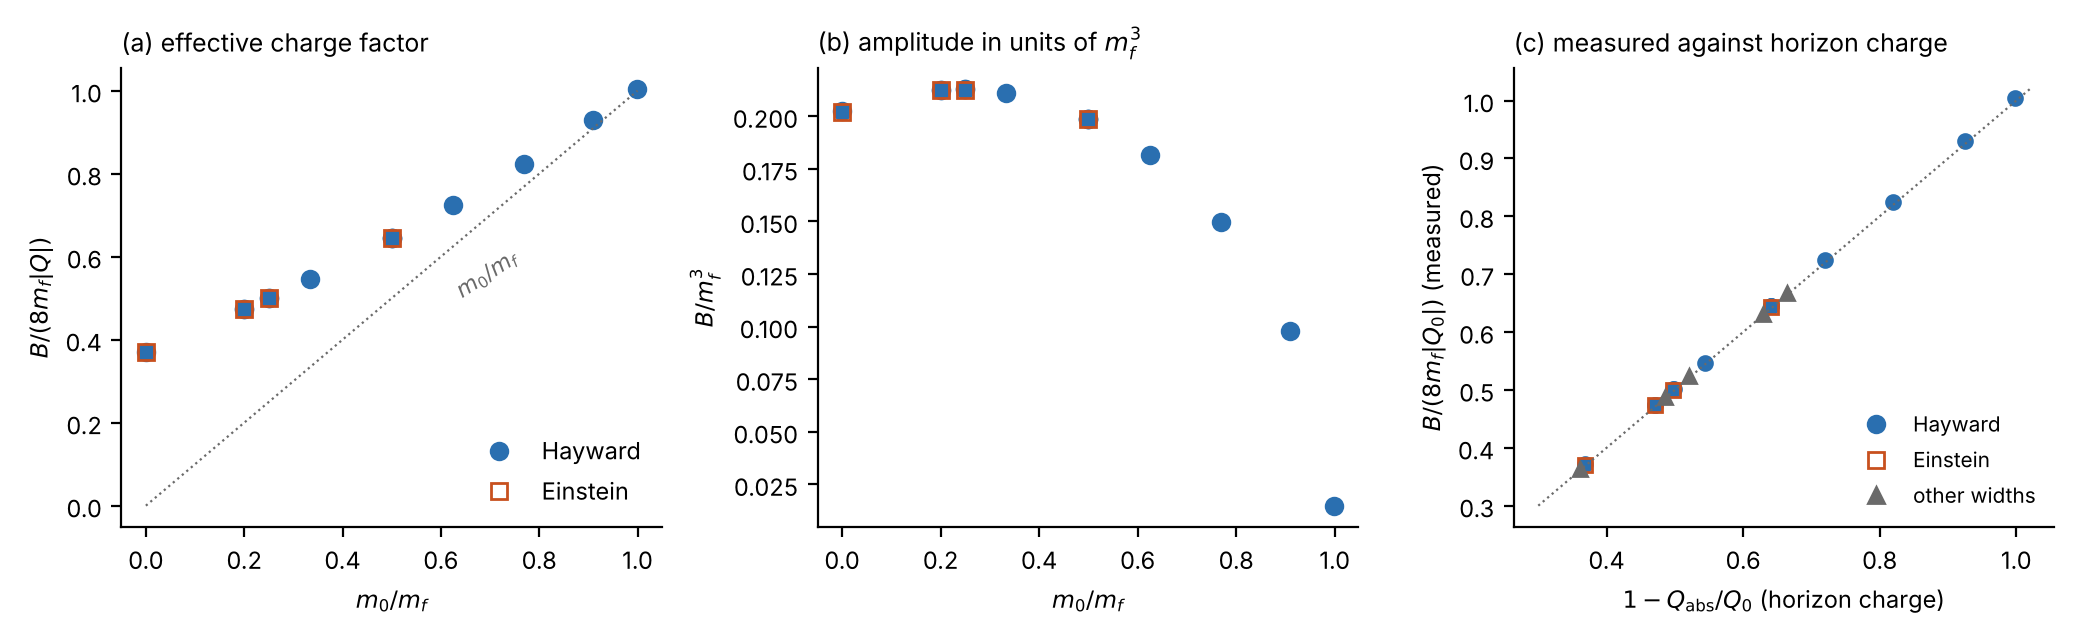
\includegraphics[width=\textwidth]{fig_strong.png}
\caption{Tails of collapse pulses into an existing hole: (a) $F=B/(8m_f|Q|)$ and (b) $B/m_f^{3}$ against $\mu=m_0/m_f$; filled circles Hayward, open squares Einstein ($m_f=5.01$ to $25$; points with equal $\mu$ and different $m_f$ coincide); (c) $F$ measured against $1-Q_{\rm abs}/Q_0$ from the charge absorbed by the event horizon, Eq.~\eqref{eq:qabs}, including pulses of other widths (the line is the identity; $B$ from the fixed-index fit, the points lie $0.56\%$ above it on average ($0.52$--$0.60\%$), and $0.05\%$ below on average ($0.09\%$ at most) with the first correction).}\label{fig:strong}
\end{figure}

\emph{Why the fold does not occur, and code~E.} The starting row of code~E is the static hole of $m_f$, which test (iii) shows is what the strong collapse leaves behind at $v_1$; the field enters code~E only through $\phi_H(v)$ after the pulse. The fold of the previous paragraph belongs to a pulse placed inside the code-E interval, where the column is shot backwards from a final state, so no event-horizon finder is needed here. Code~E on the tables for $m_0=5\to m_f=10$ and $m_0=0\to10$ ($h_s=h_v=0.2$, $v\le2000$, \texttt{MASS=10}, \texttt{PU0MODE=zero}) has the same final state: $r_\infty=1.02653$ (against $r_-(10)=1.02670$; the mass $m^{*}=10.059$ implied by $r_\infty$ agrees with the ray mass $10.055$ at the freezing time $v=94$), $zm\to0.54085$ ($\tfrac12r_\infty^{3}=0.54086$), $\mathrm dm/\mathrm dv=9.466$ over $1600\le v\le1800$ against $9.535$ from Eq.~\eqref{eq:dm} at $r_\infty$ ($0.7\%$ below), $v\sigma_v=-8.44$ and $-8.43$ and $\mathrm d\ln K/\mathrm d\ln v=10.13$ and $10.10$ at $v=1800$ ($-8$ and $10$ for $k=3$), the same for the two histories; the amplitude of $K$ differs as $B^{-4}$ ($K$ at $v=1500$: $8.98\times10^{25}$ against $8.37\times10^{25}$, ratio $1.072$, $(B_{0}/B_{5})^{4}=1.079$ for the tables' $B=198.9$ and $202.7$; \texttt{pscan\_an.py}, \texttt{pscan\_zm.py}, \texttt{pscan\_freeze.py}). For $m_f=15$ ($h_s=h_v=0.2$, $v\le2800$) $r_\infty=1.01665$ against $r_-(15)=1.01740$ (implied front mass $15.65$, $4.3\%$ above $m_f$), $zm=\tfrac12r_\infty^{3}$ to $10^{-5}$, and $\mathrm dm/\mathrm dv$ is $0.992$ of Eq.~\eqref{eq:dm} at $r_\infty$. \emph{The case $m_f=25$.} Here $r_-(25)=1.01026$ is only $1\%$ above $\ell$, and at $h_s=h_v=0.2$ the run is not converged: the implied front mass is $0.6\%$, $4.3\%$ and $92\%$ above $m_f$ for $m_f=10,\,15,\,25$ (it grows as $r_-\to\ell$, the front being under-resolved). Refining the mesh moves $r_\infty$ toward $r_-(25)$: $1.00527$, $1.00633$ ($h_s=0.1$), $1.00888$ ($h_v=0.1$) and $1.00993$ ($h_s=h_v=0.1$), i.e.\ distances from $r_-(25)$ of $5.0\times10^{-3}$, $3.9\times10^{-3}$, $1.4\times10^{-3}$ and $3.3\times10^{-4}$, implied front masses $48.1,\,40.2,\,28.8,\,25.8$ ($92\%$, $61\%$, $15\%$, $3.2\%$ above $m_f$), $zm=\tfrac12r_\infty^{3}$ to $10^{-5}$ in each, and with both meshes at $0.1$ the rate $\mathrm dm/\mathrm dv=25.21$ is $0.997$ of Eq.~\eqref{eq:dm} at $r_\infty$ (the ratios were $1.20,\,0.97,\,1.09$ on the other meshes). The bump at the front was therefore a resolution effect; at $h_s=h_v=0.1$ the case is as converged as $m_f=15$ is at $0.2$ ($4.3\%$), which is the accuracy claimed for it. What remains: no further refinement was run, $v\sigma_v=-19.8$ and $\mathrm d\ln K/\mathrm d\ln v=32.4$ at $v=2666$ ($\kappa_+v\simeq26$) are far from $-8$ and $10$ and follow the $m_f=10$ curve at the same $\kappa_+v$ ($-16.6$ and $26.6$ at $v=1200$), so the exponents are not tested at $m_f=25$ (\texttt{strong\_codeE.log}; \texttt{pscan\_freeze.py}, \texttt{pscan\_zm.py} with \texttt{VS=4.4444}).

\paragraph{What this establishes and what it does not.} The conclusions of Section~\ref{sec:curv3} (the front, the linear growth of $m$, $zm\to\tfrac12r_-^{3}/\ell^{2}$, $v\sigma_v\to-(2k+2)$ and $K\propto v^{4k-2}$ with $k=3$) hold when the horizon field is the one generated by a spherically symmetric collapse into the Hayward hole of a compact scalar pulse ($k=3$, the generic Price exponent, with the amplitude as measured, the quasi-normal transient included) or of a pulse with a $b/r^{2}$ field or a static field $c\,g(r)$ ($r\phi\to c$, $I_0=-cm$) on the initial cone ($k=2$, with $I_0=-b$ resp.\ $-cm$ and the coefficient $4I_0$ of the linear theorem; $v\sigma_v\to-6$ and $K\propto v^{4k-2}$ with $k=2$ in the sense of Section~\ref{sec:curv3}). Not established: (i) the tail for other collapse data (a thicker shell; data that are static from the center outwards rather than outside a radius, a case that requires a regular static field through the hole formed; the nonlinear value of the $k=3$ coefficient, for which only the linear identity $B=8m|Q|$ and the measured reduction are given); (ii) the full nonlinear evolution to the late times of the tail in one code (stage~L is linear on the static exterior, justified by test (a) and by the independence of the switching time, not by a nonlinear run to $v\sim10^{3}$); (iii) the interior beyond the thin layer $U\le1.5$ of the starting row and the region between the pulse and the core; (iv) the amplitude of $K$ (it depends on the profile on the starting row, and the profile used is from a nonlinear row at $v=60$ continued to the interior of that layer only); (v) the Hawking flux and the back-reaction of the Hayward collapse on the shell itself, which is not followed to the core ($u_{\rm end}<v_0$).

\section{What this establishes, what it does not, and what is next}
\label{sec:open}

\paragraph{Established, by the kind of support.}
\emph{Derived.} The generalized-mass law~\eqref{eq:mlaw} for any $h$; the sign theorem (Proposition~\ref{prop:y}) for a real scalar field and data regular on the event horizon whenever $h'>0$; the classification of Section~\ref{sec:classes}; the branch $y<0$, to which the finite-advanced-time singularity of interior characteristic data belongs, is excluded for event-horizon-regular data (existence of the solution for all $v$ is not proved).
\emph{Checked against independent computations.} The double-null equations in the Einstein limit ($10^{-16}$), on static interiors ($10^{-7}$--$10^{-6}$), through the integrability and compatibility identities ($2\times10^{-11}$, $3\times10^{-12}$; $7\times10^{-50}$ in $80$-digit arithmetic near the pole); as the Euler--Lagrange equations of the reduced action, including the $\phi_u^{2}\phi_v^{2}$ term and the Raychaudhuri coefficient $4\pi/h'$ (exact rational arithmetic); the covariant scalars $P,H,T,K$ that lift that action reduce to $\psi,\eta,\tau,\mathcal R$ on random spherical metrics ($\le8\times10^{-11}$, computed from the four-dimensional Riemann tensor, Section~\ref{sec:checks}(g)); the evolution against exact static solutions (Hayward, bounded $h$), against the $r_{uv}$ equation it does not use, against the linear-response kernel of Paper~G~\citep{PaperG}, against a second discretization (mode~2 of code~A) and against an independent fourth-order code (code~B: $10^{-7}$ in $r$ and $4\times10^{-6}$ absolute in $\sigma_v$ after the $h_s$ correction for $120\le v\le240$).
\emph{Measured.} The metric exponent $-\kappa_-(m_f)$ ($2\times10^{-6}$); the front and its delay ($13.1$ per decade of $B$ for the Hayward $h$, $13.5$ for the bounded $h$); the difference from the additive closure ($\propto B^{2}$ in the flux, $O(1)$ in $\sigma_v$ behind the front); the state behind the front for $B=3\times10^{-3}$ to $v=300$ (code~A), $v=380$ (code~B) and $v=1400$ (code~E): $\psi\to1/\ell^{2}$ with $1-\ell^{2}\psi\simeq0.59/m$, $m$ growing linearly with $\mathrm{d}m/\mathrm{d}v=3.7\to4.4$, $r\to r_-$, $\sigma_v$ rising monotonically from $-0.094$ to $-0.018$ without a zero crossing, $K$ from $10^{25}$ to $1.6\times10^{30}\ell^{-4}$ at $U\simeq1$ with a local slope of $2.5$ at $v=340$ that rises to $3.64$ at $1400$, as Eq.~\eqref{eq:kslope} predicts (and its generalization~\eqref{eq:kslopek} for $k=\tfrac12,\ldots,3$, three amplitudes and $m/\ell=3,5,10$, Section~\ref{sec:curv3}); the slaving structure of Section~\ref{sec:slave}; the error law~\eqref{eq:vb} ($28.3$ per halving of $h_v$ at second order and $56.6$ at fourth order, as $p\ln2/\kappa_+$ predicts), which moved the limit of the run from $v\approx170$ to $300$ (code~A), $380$ (code~B) and beyond $1400$ (code~E, Sections~\ref{sec:mech} and~\ref{sec:seed}); the transverse null tidal integrals over the remaining affine range ($\int\!\!\int\mathcal T\,\mathrm d\lambda^{2}\le10^{-15}$ for $v\ge300$). The tail of a collapse of a compact scalar pulse into the Hayward hole: exponent $3.009$, coefficient $B=25.45$ ($m=5$; $B/m^{3}=0.2052,\,0.2033,\,0.2015$ for $m=3,5,10$ against $0.2017$ in the Einstein limit), the static Hayward interior left behind the pulse (to $10^{-5}$ for $11\lesssim r\lesssim30$, $4\times10^{-5}$ at $r=3.8$, $1.3\times10^{-3}$ at $r=1.058$), and code~E on that tail to $v=1400$ with the exponents of Section~\ref{sec:collapse}.
\emph{Derived and tested against runs not used to fit it.} The mechanism of the error law (Section~\ref{sec:mech}): the forward integration of the horizon Raychaudhuri equation, whose one-dimensional model predicts the advanced time of failure of code~B at two other amplitudes to $0.4$ units (one fitted constant, the threshold $\delta^{*}=0.062$); the closed form~\eqref{eq:dm} for $m/\ell=3$ and $10$ ($1.5\%$ and $0.25\%$); the seed of the late-time departure of code~E (Section~\ref{sec:seed}): an offset $\epsilon$ in the initial row advances the departure by $-19.8$ per $e$-fold of $\epsilon$ over $10^{-15}$--$10^{-12}$, against $-1/\kappa_+=-20.4$.
\emph{Derived from the measured structure.} The closed forms~\eqref{eq:slave}, \eqref{eq:dm} and~\eqref{eq:kslope}, the sign $\sigma_v<0$ for a decreasing flux, and the asymptotics~\eqref{eq:asym}, which hold in the slaved description and are tested up to the simulated $v$.

\paragraph{Not established.}
(i) \emph{The endpoint and the nature of $v=\infty$.} $\sigma_v\to0^{-}$ as $-(2k+2)/v$, a finite affine range, and $K\propto v^{4k-2}$ (the local slope of $K$ is $3.64$ at $v=1400$, as Eq.~\eqref{eq:kslope} predicts; with the two $1/v$ terms of that equation removed it is $4.01$ for $k=\tfrac32$ and $0.01,\,2.01,\,6.02,\,10.02$ for $k=\tfrac12,\,1,\,2,\,3$ against $4k-2$ at $v=1021$, but the slope itself comes within $10\%$ of $4k-2$ only at the end of the simulated range, $\kappa_+v\gtrsim70$) are conjectures about $v\to\infty$ based on a verified structure; extendibility of the metric, the strength of the singularity for timelike observers, and linear perturbations of the solution at $v=\infty$ are not studied.
(ii) \emph{Parameters.} Tail exponents $k=\tfrac12,1,\tfrac32,2,3$ (prescribed on the horizon in Section~\ref{sec:curv3}; Section~\ref{sec:collapse} generates $k=3$ and its amplitude from a collapse of a compact pulse, and $k=2$ from collapse data with $I_0\ne0$ ($r\phi\to0$ and $r\phi\to c$ at infinity); code~E is driven by the $k=3$ and the $b/r^{2}$ $k=2$ horizon fields, not by the $r\phi\to c$ one, whose horizon field is the same to $10^{-4}$ in the coefficient), amplitudes $3\times10^{-4}$--$3\times10^{-2}$ and inner masses $m/\ell=3,5,10$ with code~E to $\kappa_+v\simeq50$--$69$ (Section~\ref{sec:curv3}; the equations depend on $m/\ell$ only); with code~A $k=\tfrac12,\tfrac32,3$ (windows $v\simeq160$--$380$) and $m=3$ ($zm\to0.677$); for the bounded $h$ one value of $m/\sqrt\alpha$, a window $v\lesssim125$, no kernel and no run of code~E. Codes~B and~E were run for the Hayward $h$ only.
(iii) \emph{The theory.} The four-dimensional theory, its Hayward resummation and the analytic continuation of the time-dependent equations outside $0<\psi<1/\ell^{2}$ are taken from Refs.~\cite{BuenoCanoHennigarMurcia2025,BorissovaCarballoRubio2026}; the lifts are non-polynomial and not unique (Section~\ref{sec:checks}(g)), and the denominators of $I_{C^{2}}$ vanish on conformally flat configurations, which the solution behind the front avoids ($\Omega\ge8\times10^{11}$); hyperbolicity and well-posedness of the full (non-spherical) theory are not studied. For the spherical sector the system~\eqref{eq:ray}--\eqref{eq:phi} has the form $X_{uv}=F(X,X_u,X_v)$ for $X=(r,\sigma,\phi)$ plus two constraints, with $F$ smooth for $0<\psi<1/\ell^{2}$, $r>0$, $W>0$, i.e.\ a Goursat problem whose characteristics are $u,v=\mathrm{const}$ whatever the size of $c_3\phi_u^{2}\phi_v^{2}$; the change from hyperbolic to elliptic type that \citet{RipleyPretorius2019} find in shift-symmetric Einstein-dilaton-Gauss--Bonnet collapse requires a derivative coupling of the scalar and has no counterpart for this minimally coupled scalar as long as $\psi<1/\ell^{2}$ (an observation about the form of the equations, not a theorem about their solutions; the coefficients degenerate at the pole of $h$, which the solution approaches as $1/v$). The equations, not only the scheme, are untested by a code in a different gauge or variables. The solution is very sensitive to the $c_3$ term ($10\%$ moves $\sigma_v$ by $0.024$ at $v=70$; without it there is no front), which is fixed by the action.
(iv) \emph{Validity.} A curvature of $10^{25}$--$10^{28}\ell^{-4}$ is far outside the regime of a classical four-dimensional effective theory; the result is the classical evolution of the theory with a minimally coupled scalar. In particular the dynamical curvature bound that holds for static solutions (the limiting-curvature property) does not hold for this matter coupling.
(v) \emph{Physics not included.} The Hawking flux, matter other than a massless scalar, charge and rotation, and any thin-shell (Ori) argument: Di~Filippo, Kubi\v{z}n\'ak and Srinivasan~\cite{DiFilippo2026} find that null thin shells are not available in the standard distributional theory for vacuum regular black holes of this kind, whereas Ref.~\cite{FrolovZelnikov2026} uses them with junction conditions; we take no side.
(vi) \emph{The numerics.} The error law is derived (Section~\ref{sec:mech}), but the threshold $\delta^{*}=0.062$ is a fitted constant (from the five failure times of code~B at $B=3\times10^{-3}$) and is not derived; the former limit of code~E, a step in the initial row amplified at the rate $\kappa_+$ from $\kappa_+v\simeq33$, is located and removed (Section~\ref{sec:seed}), and no other limit appears to $\kappa_+v=69$, but no run beyond that has been made; the free (unconstrained) evolution fails in both codes by $v\simeq100$ and that mechanism is not analyzed.
(vii) \emph{The tail coefficient of the strong collapse.} The identification of $Q_{\rm abs}$ with the horizon term of the time-inverted Newman--Penrose constant of Gajic and Kehrberger~\citeyearpar{GajicKehrberger2025} is conditional: the hypotheses of their theorem (a given metric settling to Schwarzschild at a polynomial rate, smooth compactly supported data) were not verified for the collapse data, the final exterior of the Hayward model is not Schwarzschild, and of that paper the energy estimates of Section~5 and the iteration of Sections~7.4--7.8 were not read (see Section~\ref{sec:collapse}). The agreement of $F$ with $1-Q_{\rm abs}/Q_0$ ($0.05\%$ on average) is a numerical fact about our runs; the a priori estimates of $Q_{\rm abs}$ (Vaidya-like horizon, eikonal field; low by $1.5\%$ and $2.3\%$ on average, $3.6\%$ and $4.1\%$ at most, in the same $22$ cases) are empirical figures and not bounds.

\paragraph{Consequence for the series.} The question left open by Paper~E~\citep{PaperE}, whether the mass-tracking metric can be tested nonlinearly, has a partial answer. In the theory that realizes its static sector, with data regular on the event horizon, the metric exponent follows the generalized mass accumulated on the horizon, as in the additive closure; the flux through the interior is the linear response of the static interior (Paper~G) up to a correction quadratic in the tail amplitude; then a front arrives, behind which the generalized mass inflates linearly in $v$, $\psi$ approaches the pole of $h$ without reaching it, the Misner--Sharp mass stays at $\tfrac12r_-^{3}/\ell^{2}$, $r$ stays at $r_-$, the exponent $\sigma_v$ is slaved to the flux and rises toward zero from below, and the curvature, carried by the term of the theory quartic in the scalar gradient, is far above $\ell^{-4}$ and grows with a slowly varying power of $v$. This differs from the additive closure of Papers~E and~G~\citep{PaperE,PaperG}, where the Misner--Sharp mass inflates and $\sigma_v$ keeps the exponent $-\kappa_-(\mu_f)$. The inner horizon of the Hayward interior is thus unstable in this theory in the sense that the generalized mass grows linearly and the curvature as a power of $v$ while the Misner--Sharp mass and $r$ stay bounded; the geometry behind the front is neither the static interior nor the singular branch of interior data; in the slaved continuation (power-law tail completion) the accumulated transverse tidal distortion along radial null geodesics on the ray stays finite and small.

\paragraph{Next steps.} (1) The strong collapse pulse at $m_f>25$ (where $r_-\to\ell$ and the front needs $h\le0.1$ and a still finer mesh, $h=0.05$, for the exponents), an estimate of the absorbed charge $Q_{\rm abs}$ (Eq.~\eqref{eq:qabs}) better than the $2$--$4\%$ observed in the $22$ cases (an empirical figure, not a bound) of the Vaidya-eikonal one (scattering of the pulse by the hole), and an event-horizon finder for pulses that do not end in a static hole; a thicker shell, initially static fields through the center, a collapse followed to the core, and an a priori value of the nonlinear $v^{-3}$ coefficient, the full nonlinear evolution to $v\sim10^{3}$ in one code (a grid adapted to the horizon), the dependence of the amplitude of $K$ on the interior profile, the kernel of the bounded model, and the bounded $h$ with code~E. (2) Timelike geodesics and the singularity strength at $v=\infty$, and the question whether a null thin shell regularizes or strengthens the front. (3) A continuation criterion for the spherical Goursat system (the solution exists as long as $\psi$ stays below $1/\ell^{2}$ and $r$, $W$ stay positive) and the hyperbolicity of the non-spherical theory, which is the open one. (4) A code in the gauge $\varphi=r$ of Ref.~\cite{BuenoCanoHennigarMurcia2025}. (5) Non-minimally coupled matter that restores a curvature bound (Ref.~\cite{BuenoHennigarMurciaVicenteCano2026}) and its effect on the front. (6) The Hawking flux (a separate study). (7) Code~E beyond $\kappa_+v\simeq70$ ($v\gtrsim1.5\times10^{3}$ for $m/\ell=5$), to see whether a further rounding-level seed exists and to reach the regime where the slope of $K$ itself is within a few percent of $4k-2$.

\paragraph{Level of reading of the sources.} We use the time-dependent equations of Ref.~\cite{BuenoCanoHennigarMurcia2025} (Eqs.~(36)--(38)) and the characteristic functions (Eq.~(51) for the bounded model there); the static identification of the Hayward metric with $h=\psi/(1-\ell^{2}\psi)$ and the covariant densities (Eqs.~(53)--(66)) are those of Ref.~\cite{BorissovaCarballoRubio2026}, checked here directly (Section~\ref{sec:theory} and~\ref{sec:checks}(g)). Of Ref.~\cite{BorissovaCarballoRubio2026} the text was read through its Eq.~(156); the rest of its Section~IV and its Discussion were not, and the statement about Ref.~\cite{DiFilippo2026} rests on its abstract. Refs.~\cite{BuenoCanoHennigar2024,BuenoCanoHennigarMurcia2024,FrolovZelnikov2026,DiFilippo2026,CarballoRubio2022a,BuenoHennigarMurciaVicenteCano2026,BonannoPanassitiSaueressig2025,ShaoGuoTianZhang2025,Iofa2022} are used at the level of the abstract and the statements attributed to them; we have not checked their numerical results. Refs.~\cite{PoissonIsrael1989,PoissonIsrael1990,Dafermos2005,Ori1991,BradySmith1995,Burko1997,HodPiran1998,MarolfOri2012} are cited for the mass-inflation context. Ref.~\citep{GajicKehrberger2025}, which Section~\ref{sec:collapse} uses, was read in part: the abstract, Section~1 (Theorem~1.1, Eqs.~(1.5)--(1.8), Remarks~1.1--1.3, footnotes~1 and~2, Section~1.1.4 and the sketch of Section~1.2), Sections~2 and~3 and the statements of Section~4 (Assumptions~4.1 and~4.2, Theorems~4.1--4.5, Remarks~4.1--4.15); the derivation of the $\ell=0$ constant (Proposition~7.1, Lemma~7.2), Sections~6, 8 and~9 and the appendices were also read; the energy estimates of Section~5 and the iteration of Sections~7.4--7.8 were not. Ref.~\citep{Gautam2024} was read through the statements of its Theorems~1.1 and~1.15 in the introduction, Ref.~\citep{BizonChmajRostworowski2008} for its Eqs.~(23), (25), (28), (34) and~(35), and Ref.~\citep{GundlachPricePullin1994b} for the exponents quoted. The identification of $Q_{\rm abs}$ with the horizon term of the time-inverted Newman--Penrose constant of Gajic and Kehrberger is conditional: the hypotheses of their theorem (a given metric settling to Schwarzschild at a polynomial rate, smooth compactly supported data, weak global decay of $\phi$) were not verified for the collapse data, the final exterior of the Hayward model is not Schwarzschild (Assumption~3.1 requires $g-g_M\lesssim\tau^{-1-\delta}$ up to the horizon), and the energy estimates of Section~5 and the iteration of Sections~7.4--7.8 of that paper were not read. For $m=5$, $\ell=1$ one has $r_+=9.898$ against $2m=10$: with the null coordinates of $g$ and $g_M$ identified and $r_*$ matched at infinity, $\not g_{AB}-(\not g_M)_{AB}\to(r_+^{2}-4m^{2})\mathring g_{AB}=-2.03\,\mathring g_{AB}$ on $\mathcal H^{+}$ for all $\tau$, so that Eq.~(3.6) fails for every $\delta>0$, and so does the weaker form $g-g_M\lesssim r^{-1}\tau^{-\delta}$ of their Remark~4.6; choosing $M=r_+/2$ instead violates the Bondi normalization (an $r^{-1}$ term $-2(m-M)/r$ in $\Omega^2-\Omega_M^2$). The expansions along $\mathcal I^{+}$ are not the obstruction. The Hayward coefficient therefore rests on the numerical result $B/(8m|Q|)=1.000$ to $10^{-3}$ and on the stationary theory of \citet{AngelopoulosAretakisGajic2018}, whose hypotheses on $f$ we have not checked.

\appendix
\section{Interior characteristic data: the ray tests}
\label{sec:num}

Before event-horizon-regular data are available (Section~\ref{sec:ehdata}), the equations can be tested on characteristic data given on interior rays, as in the nonlinear test of Paper~E~\citep{PaperE}. This section reports those runs. Their role changes after Proposition~\ref{prop:y}: they are tests of the ray equations and of the scheme, and the singular behavior they show belongs to the data.

\paragraph{Scheme and data.} We solve~\eqref{eq:ruv}--\eqref{eq:phi} for $(r,\sigma,\phi)$ with the second-order scheme of Paper~E (predictor--corrector on the null diamond, three corrector iterations; \texttt{qtg\_dn.c}), in the streaming form that stores only selected columns $u=$ const. The data are characteristic data inside the hole as in the nonlinear test of Paper~E: the static Hayward interior ($m=5$, $\ell=1$; $\sigma$ static on both rays), $\phi=B+A\,e^{-u^{2}}$ on $v=0$ ($A=0.02$) and the power-law tail $\phi=B(1+v)^{-k}$ on $u=u_0=-6$ ($k=3/2$ unless noted); $r$, $r_u$, $r_v$ and the $\sigma$-derivatives on the data rays follow from~\eqref{eq:ray}--\eqref{eq:ruv} along the rays by an ODE integration to $10^{-12}$. These are not data regular on the event horizon (Section~\ref{sec:ehdata}); they are the data of the $(u,v)$ runs of Paper~E, for which the additive closure gave mass inflation at finite radius.

\paragraph{The data ray.} On the ray $u=u_0$ the ray ODE is closed (the data are the tail $\phi_v(v)$ and the static $\sigma_v$ of the data surface). We integrate it to the event $|\psi|>10^{6}$ (\texttt{ray\_blowup.py}, \texttt{ray\_blowup.log}) and find
\begin{center}\small
\begin{tabular}{cccccccc}
\toprule
$B$ & $2\!\times\!10^{-2}$ & $2\!\times\!10^{-3}$ & $2\!\times\!10^{-4}$ & $2\!\times\!10^{-5}$ & $2\!\times\!10^{-6}$ & $2\!\times\!10^{-7}$\\\midrule
$v_*$ & $46.5$ & $57.3$ & $70.1$ & $82.8$ & $95.2$ & $107.6$\\
$r-r_-$ at $v_*$ & $-0.56$ & $-5.6\!\times\!10^{-3}$ & $-5.6\!\times\!10^{-5}$ & $-5.6\!\times\!10^{-7}$ & $-5.6\!\times\!10^{-9}$ & $-5.6\!\times\!10^{-11}$\\\bottomrule
\end{tabular}
\end{center}
with $\psi(v_*)=-10^{6}$ (the event) in every case: $v_*$ increases by $12.3$ per decade of $B$ in a linear fit over the six values (local slopes $12.8,\,12.6,\,12.5,\,12.3$ per decade, i.e.\ $5.58\to5.36$ per $e$-fold of $1/B$), i.e.\ logarithmically, as expected for a quantity that grows like $e^{\lambda v}$ from an initial value $\propto B$ or $B^{2}$; we have not derived $\lambda$ (a rate $\lambda\simeq1/5.4$ would fit an initial departure $\propto B$). The negative sign of $r-r_-$ is the Hayward curvature singularity of Section~\ref{sec:classes}(ii): the ray has crossed below $r_-$ by an amount $\propto B^{2}$ at $v_*$ (the tabulated differences fall by $10^{2}$ per decade of $B$), and in the limit $B\to0$ the singular radius tends to $r_-$. The dependence on the tail exponent at $B=2\times10^{-3}$ is weak: $v_*=51.5,\,53.6,\,57.3,\,61.8,\,72.1$ for $k=0.5,\,1,\,3/2,\,2,\,3$. For comparison the Einstein-additive ray ODE of Paper~E has no finite-$v$ singularity at this stage ($M\sim e^{\kappa_-v}$ at finite radius to $v=3000$).

\paragraph{Classification of rays.} \texttt{run\_scan\_u.py} scans $u\in[-5,6]$ at $B=2\times10^{-4}$ (table below; $h=0.0025$; the values at $v=64$ are converged to about $10^{-3}$ in $\psi$ on $y>0$ rays and are quoted mainly for the sign of $y$; see Appendix~\ref{app:res}). The sign of $y=-r_u/W$ is negative for $u\le-2$ and positive for $u\ge-1$, as in Paper~E (there $u_\star\in[-2.04,-1.0]$ for the additive closure); on the $y<0$ rays $\psi$ stays at the static value $1/r_-^{2}=0.8943$ until $v\sim60$ and then decreases, on the $y>0$ rays $\psi$ rises toward $1/\ell^{2}=1$ (and $\sigma_v$ rises from $-\kappa_-$ toward $0$), as~\eqref{eq:mlaw} predicts for the two signs.

\begin{center}\small
\begin{tabular}{rcccccc}
\toprule
$u$ & sign $y$ & $\psi(40)$ & $\psi(56)$ & $\psi(60)$ & $\psi(64)$ & $\sigma_v(60)$, $\sigma_v(64)$\\\midrule
-5 & $-$ & 0.8943 & 0.8943 & 0.8942 & 0.8930 & -0.796, -0.796\\
-4 & $-$ & 0.8943 & 0.8943 & 0.8942 & 0.8929 & -0.796, -0.796\\
-3 & $-$ & 0.8943 & 0.8942 & 0.8942 & 0.8928 & -0.796, -0.796\\
-2 & $-$ & 0.8943 & 0.8943 & 0.8942 & 0.8936 & -0.795, -0.782\\
-1 & $+$ & 0.8950 & 0.8966 & 0.9136 & 0.9532 & -0.564, -0.197\\
0 & $+$ & 0.8977 & 0.9069 & 0.9435 & 0.9694 & -0.294, -0.111\\
1 & $+$ & 0.8984 & 0.9107 & 0.9488 & 0.9714 & -0.258, -0.102\\
2 & $+$ & 0.8988 & 0.9131 & 0.9515 & 0.9724 & -0.240, -0.098\\
4 & $+$ & 0.8989 & 0.9135 & 0.9517 & 0.9722 & -0.237, -0.097\\
6 & $+$ & 0.8989 & 0.9147 & 0.9524 & 0.9716 & -0.227, -0.094\\
\bottomrule
\end{tabular}
\end{center}


\paragraph{The $y<0$ side in the evolution.} The data ray is the first to reach $v_*(u_0)$, and the evolved solution cannot be continued past it on any rectangle $[u_0,u_1]\times[0,v]$. Below that time the interior $y<0$ rays behave as~\eqref{eq:mlaw} requires: at $B=2\times10^{-3}$ ($v_*(u_0)=57.3$) the run to $v=56.5$ on $h=0.02$ gives $\psi$ passing a maximum of $0.894$--$0.896$ at $v\approx32$ (its static value is $1/r_-^{2}=0.8943$) and then decreasing monotonically to $0.855$, $0.853$, $0.852$, $0.850$, $0.846$ at $v=55.5$ on $u=-6,\,-5,\,-4,\,-3,\,-2$, with no $|\psi|>10^{3}$ anywhere, while the $y>0$ rays rise to $0.905$--$0.945$ (\texttt{run\_pde\_blowup2.py}, \texttt{pde\_blowup\_h0.02.log}; $h=0.02$ is not a converged mesh at these times, and the statement is qualitative). We have not evolved the interior rays through their own singular times; that would need data on a surface that is regular beyond $v_*(u_0)$.

\paragraph{Reading after Proposition~\ref{prop:y}.} The rays with $y<0$ above arise because the characteristic data on $u=u_0$ and $v=0$ do not come from a surface regular on the event horizon: their $y$ is whatever the static interior and the pulse at $u\sim0$ give, and it is negative for $u\le-2$. For event-horizon-regular data $y\ge\tfrac12$ and the negative-mass branch cannot occur. The finite-advanced-time singularity of this section is therefore an artifact of the data, and it should not be read as the fate of the interior of the Hayward metric in this theory. What these runs do establish is that the ray equations behave as~\eqref{eq:mlaw} requires for both signs of $y$ and that the scheme is second-order convergent (Section~\ref{sec:checks}).

\paragraph{Bounded $h$ on interior data.} For the bounded $h$ of~\eqref{eq:hB} with $\alpha=1$ and $m=1$ ($r_-=1.0927$, $\kappa_-=0.5054$, $\psi(r_-)=0.8376$) the same data ($A=0.02$, $B=2\times10^{-3}$, $k=3/2$) run to $v=76$ at $h=0.02$ without any failure (\texttt{run\_model2.py}, \texttt{model2\_h0.02.log}), well beyond the $v_*$ of the Hayward $h$ for the same data ($57.3$), and $\psi$ stays inside the wall: its range over the whole grid is $[0.326,\,0.9727]$. On the rays $u=-6,\,-3$ ($y<0$, $y\simeq-9\times10^{11}$ at $v=76$) $\psi$ falls from $0.8376$ to $0.771$, $0.770$ (the generalized mass decreasing, as~\eqref{eq:mlaw} says, so that $\psi$ moves toward the lower wall $-1/\alpha$, which is far), while on $u=0,\,2,\,4,\,6$ ($y>0$, $y\simeq1.7$--$1.9\times10^{12}$) $\psi$ rises to $0.959$, $0.9726$, $0.9726$, $0.9724$ and $\sigma_v$ rises from $-\kappa_-=-0.505$ to $+0.003,\,+0.026,\,+0.026,\,+0.026$. The picture is that of the Hayward $y>0$ side: $\psi$ goes to the positive wall (here $1/\alpha=1$) as the generalized mass grows, $\sigma_v$ rises through zero. The convergence is second order for both models (Section~\ref{sec:checks}). The Hayward and the bounded $h$ therefore agree qualitatively on the positive-mass side and differ on the negative-mass side, exactly where the range of $h$ differs.

\begin{figure}[t]
\centering
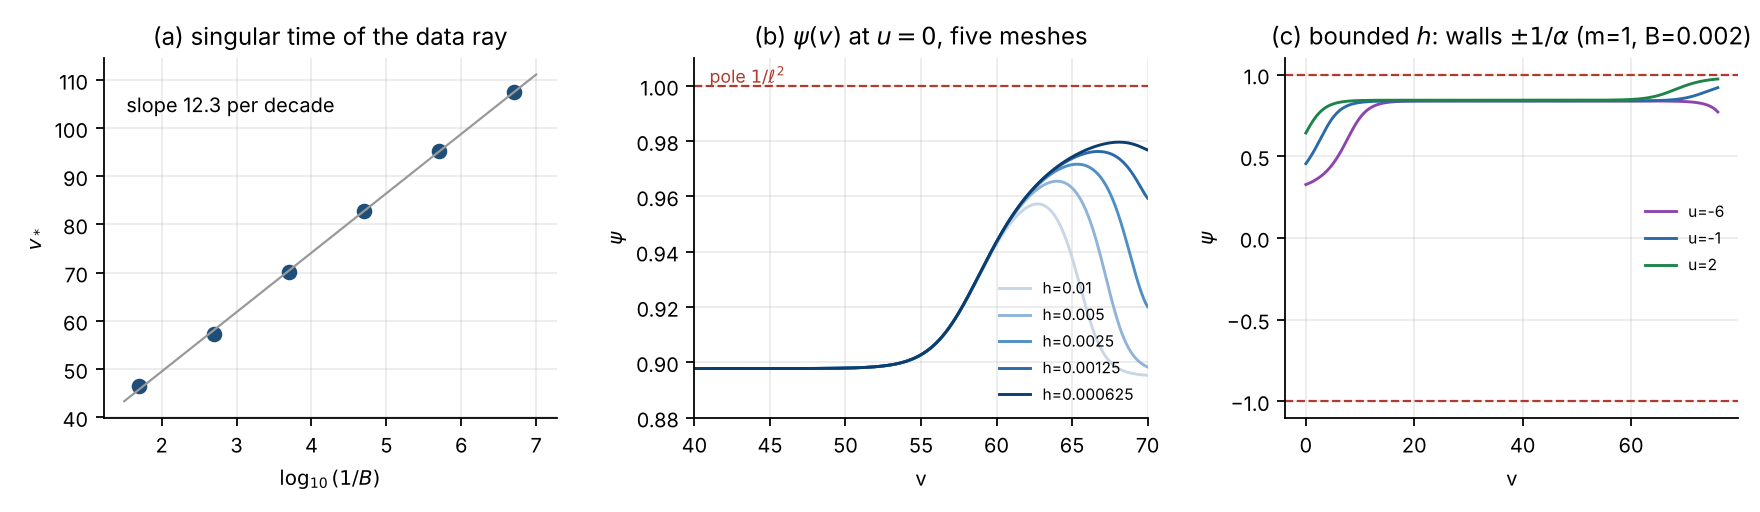
\includegraphics[width=\textwidth]{fig_qtg.png}
\caption{(a) Advanced time $v_*$ at which $|\psi|$ reaches $10^{6}$ on the data ray $u=u_0$ against $\log_{10}(1/B)$ (Hayward $h$, $k=3/2$); the line is the linear fit of Appendix~\ref{sec:num}. (b) $\psi(v)$ at $u=0$ for $B=2\times10^{-4}$ on five meshes; the pole of the Hayward $h$ is $1/\ell^{2}=1$. (c) Bounded $h$ ($m=1$, $\alpha=1$, $B=2\times10^{-3}$, $h=0.02$): $\psi$ on rays with $y<0$ ($u=-6$) and $y>0$ ($u=-1,\,2$) stays within the walls $\pm1/\alpha$.}
\label{fig:qtg}
\end{figure}


\section{Curvature invariants in double-null form}
\label{app:curv}

For $ds^{2}=g_{ab}dx^{a}dx^{b}+r^{2}d\Omega^{2}$, with $g=-W\,du\,dv$, the Kretschmann invariant is $K=R_2^{2}+8\,H_{ab}H^{ab}/r^{2}+4(1-(\nabla r)^{2})^{2}/r^{4}$, with $R_2$ the curvature scalar of the two-metric and $H_{ab}=\nabla_a\nabla_br$. Here $(1-(\nabla r)^{2})/r^{2}=\psi$ and $R_2=4\sigma_{uv}/W\equiv4\Sigma$. With $\Gamma^{u}_{uu}=\sigma_u$, $\Gamma^{v}_{vv}=\sigma_v$ one has $H_{uu}=r_{uu}-\sigma_ur_u$, $H_{vv}=r_{vv}-\sigma_vr_v$, $H_{uv}=r_{uv}$, and $g^{uv}=-2/W$, so $H_{ab}H^{ab}=(8/W^{2})(H_{uu}H_{vv}+H_{uv}^{2})$. Using~\eqref{eq:ray}, \eqref{eq:ruv}: $H_{uu}H_{vv}=16\pi^{2}r^{2}c_1^{2}\phi_u^{2}\phi_v^{2}$ and $H_{uv}^{2}=W^{2}r^{2}Q^{2}/16$, which gives~\eqref{eq:kret}, and $\Sigma$ follows from~\eqref{eq:suv}. The formula reproduces $48M^{2}/r^{6}$ for the Schwarzschild metric and $24/\ell^{4}$ at the Hayward pole with no flux, and agrees with $f''^{2}+4f'^{2}/r^{2}+4(1-f)^{2}/r^{4}$ on the static interiors (\texttt{check\_curv\_static.log}). It is a geometric statement about the metric $(r,\sigma)$ that was evolved; it depends on $h$ through $Q,c_1,c_2,c_3$.

\section{Resolution study of the interior-data run}
\label{app:res}

\paragraph{Resolution study at $u=0$.} The $y>0$ side is where $\psi$ approaches the pole $1/\ell^{2}$, and where the scheme is most demanding. Table~\ref{tab:conv} gives $\psi$ and $\sigma_v$ at $u=0$ for $B=2\times10^{-4}$ on five meshes. At $v\le60$ the solution is converged to $5\times10^{-5}$ in $\psi$ and $6\times10^{-4}$ in $\sigma_v$ already at $h=0.0025$. At $v=64$ the successive differences in $\psi$ are $1.37\times10^{-2}$, $3.9\times10^{-3}$, $1.0\times10^{-3}$, $2.6\times10^{-4}$, with ratios $3.5,\,3.9,\,3.9$, i.e.\ second order, and the two finest meshes differ by $2.6\times10^{-4}$ in $\psi$ and $2.6\times10^{-3}$ in $\sigma_v$. The coarse meshes ($h\ge0.005$) show a spurious maximum of $\psi$ near $v=64$--$66$ followed by a decrease and a spurious sign change of $\sigma_v$; this is a resolution artifact (the converged $\psi$ increases monotonically through $v=68$). At $v=68$ the two finest meshes still differ by $5.5\times10^{-3}$ in $\psi$ ($\sigma_v=+0.169$ against $+0.120$): the solution is not converged there. As an independent diagnostic we evaluate the exact identity~\eqref{eq:psiv} on the stored columns (\texttt{check\_psi\_identity.py}): the defect of $\partial_v\psi$ relative to the largest term is $2.1\times10^{-3}$, $0.39$, $2.8$ for $h=0.01$ and $5.9\times10^{-5}$, $1.6\times10^{-3}$, $6.1\times10^{-2}$ for $h=0.000625$ in $v\in[40,56],\,[56,62],\,[62,66]$ (falling by about $4$ per halving in the middle window), so the $\psi$-equation is satisfied to $2\times10^{-3}$ for $v\le62$ at the finest mesh and to $6\%$ in $[62,66]$.
\begin{table}[ht]\centering\small
\caption{$\psi$ and $\sigma_v$ at $u=0$ ($B=2\times10^{-4}$, $A=0.02$, Hayward $h$) on five meshes (\texttt{run\_conv.py}, \texttt{conv\_B2e-4.log}).}\label{tab:conv}
\begin{tabular}{rcccccc}
\toprule
$h$ & $\psi(56)$ & $\psi(60)$ & $\psi(64)$ & $\psi(66)$ & $\psi(68)$ & $\sigma_v(64)$, $\sigma_v(68)$\\\midrule
0.01 & 0.90684 & 0.94268 & 0.95176 & 0.91842 & 0.89799 & +0.0939, +1.1879\\
0.005 & 0.90691 & 0.94337 & 0.96550 & 0.95392 & 0.91531 & -0.0705, +0.9805\\
0.0025 & 0.90693 & 0.94355 & 0.96942 & 0.97093 & 0.95445 & -0.1114, +0.3855\\
0.00125 & 0.90693 & 0.94359 & 0.97042 & 0.97575 & 0.97413 & -0.1215, +0.1687\\
0.000625 & 0.90693 & 0.94360 & 0.97068 & 0.97698 & 0.97962 & -0.1241, +0.1197\\
\bottomrule
\end{tabular}
\end{table}

We do not claim a converged late-time endpoint for $y>0$: the converged range is $v\lesssim64$ ($\psi=0.971$, $\sigma_v=-0.12$ at $v=64$), the finest mesh gives $\psi=0.980$ and $\sigma_v=+0.12$ at $v=68$ with the $5\times10^{-3}$ uncertainty stated above, and the singular behavior on the $y<0$ side (which sets $v_*\simeq70$ for this amplitude) is the limit on useful $v$ for any run in this setup. Whether $\sigma_v\to0^{+}$ and the $y>0$ side tends to a regular configuration with $\psi\to1/\ell^{2}$, as~\eqref{eq:mlaw} suggests for $m\to\infty$, or something else, is open.


\section*{Code and data availability}
\raggedright
All code, logs and data tables behind the numbers and figures of this paper are archived at Zenodo, doi:\href{https://doi.org/10.5281/zenodo.23455595}{10.5281/zenodo.23455595}, (code: MIT license; text, figures and data: CC-BY-4.0). The archive is self-contained: the modules of Paper~E that it needs are copied in \texttt{code/vendor\_E/} (copied from the Paper~E archive, doi:\href{https://doi.org/10.5281/zenodo.23455587}{10.5281/zenodo.23455587}~\citep{PaperE}), and no other directory is required. It needs Python~3 with numpy, scipy and matplotlib and a C compiler (\texttt{requirements.txt}). \texttt{code/README.md} gives the dependency graph of the scripts, one measured run time per script and the logs that have no generator in the archive. \texttt{code/eh\_qtg/run\_analysis.sh} re-runs the analysis scripts and compares each new log with the shipped one (\texttt{ONLY=<substring>} selects scripts, \texttt{RUN\_LONG=1} adds the long evolutions). \texttt{bash verify.sh} in the archive runs 162 quick-tier jobs (about 55 CPU-minutes) and, with \texttt{--full}, 40 further long jobs; it compares 2149 quoted numbers with the computed ones and writes \texttt{verification/REPORT.md}; \texttt{B\_ASYM=1.5} is the default for the \texttt{asym1} fits.
\raggedright
Interior-data runs (Sections~\ref{sec:checks} and~\ref{sec:num}): \texttt{code/run\_all.sh} regenerates every log quoted there. \texttt{qtg\_dn.c} is the C evolution routine (\texttt{evolve\_qtg}, \texttt{evolve\_stream\_qtg} with models $0,1,2$ and, new here, \texttt{evolve\_stream\_qtg\_cy}, the constrained evolution of Section~\ref{sec:cy} with modes 1--3); \texttt{qtg\_lib.py} the Python side (data, ray ODE, \texttt{coef}, \texttt{hfun}, \texttt{run\_stream\_cy}); \texttt{qtg\_bg2.py} the static interior of the bounded model; \texttt{check\_*.py} the checks of Section~\ref{sec:checks}; \texttt{ray\_blowup.py}, \texttt{run\_scan\_u.py}, \texttt{run\_conv.py}, \texttt{run\_model2.py}, \texttt{run\_pde\_blowup2.py} Appendix~\ref{sec:num}; \texttt{make\_figs.py} its figure.
Code~E, the mechanism, the seed and the scans (Sections~\ref{sec:mech}, \ref{sec:seed} and~\ref{sec:curv3}): \texttt{code/eh\_qtg/codee/} (\texttt{qtg\_e.c}, \texttt{qtg\_el.c} in long double, \texttt{gen\_e.py}, \texttt{t\_static\_e.py}, \texttt{mech\_vb.py} and \texttt{vb\_prediction.py}, \texttt{conv\_e.py}, \texttt{conv\_e2.py}, \texttt{seed\_amplitude.py}, \texttt{noise\_tests.py}, \texttt{scan\_an.py}, \texttt{scans.sh}, \texttt{kstudy2.py}; thinned data in \texttt{data/}, logs in \texttt{logs/}; \texttt{setup.sh} builds the libraries).
Event-horizon-regular runs (Sections~\ref{sec:ehdata}--\ref{sec:model2}): \texttt{code/eh\_qtg/} (README there). \texttt{setup.sh} builds the three evolution libraries and the data-construction library from the modules in \texttt{code/vendor\_E/} (no sibling directory is needed); \texttt{run\_eh.sh} regenerates the logs in \texttt{logs/} (the runs are independent; the longest are the runs on four meshes to $h=0.00625$ for three amplitudes and two models). The modules: \texttt{static\_gen.py} (exact static solution for any $f$), \texttt{dnU\_qtg.py} (horizon data and rows), \texttt{gen\_q.py} (four-mesh runs, writes the JSON in \texttt{data/}), \texttt{analyze\_q.py} (Romberg extrapolation); the analyses \texttt{late\_q.py}, \texttt{endpoint\_q.py}, \texttt{front\_q.py}, \texttt{width\_q.py}, \texttt{plateau\_q.py}, \texttt{kap\_check.py}, \texttt{kap\_check\_b.py}, \texttt{kernel\_ratio\_q.py}, \texttt{cmp\_add.py}, \texttt{masslaw\_q.py}, \texttt{curv\_q.py}, \texttt{curv\_terms\_q.py}, \texttt{check\_curv\_static.py}, \texttt{check\_ruv\_q.py}, \texttt{t\_static\_*.py}, \texttt{free\_vs\_con.py}, \texttt{fig\_eh.py}. The JSON files shipped are the extrapolation inputs.

\paragraph{Collapse-generated tails (Section~\ref{sec:collapse}).} \texttt{code/eh\_qtg/codec/}: \texttt{qtg\_col.c} (stage~N: free evolution of \texttt{qtg\_dn.c} with row snapshots and an apparent-horizon tracker), \texttt{qtg\_L.c} and \texttt{tail\_L.py} (stage~L and the static Hayward/Schwarzschild background in closed form), \texttt{collapse\_lib.py} (data on the two rays), \texttt{pipeline.py}, \texttt{collapse\_tail.py} (the table of $\phi_H(v)$), \texttt{gen\_c.py} (code~E driven by a table; needs \texttt{eh\_qtg/setup.sh}), the tests \texttt{interior.py}, \texttt{overlap.py}, \texttt{tables.py}, \texttt{mscale.py}, \texttt{ascale.py}, \texttt{linear.py}, \texttt{fit\_tables.py}, the analyses \texttt{front.py}, \texttt{collapse\_E.py}, \texttt{conv\_c.py}, \texttt{fig\_collapse.py}; \texttt{run\_all.sh} regenerates the logs of stages~N and~L (the data of the runs quoted are in \texttt{data/}). The $k=2$ data of Section~\ref{sec:collapse}: \texttt{nplin.py} (stage~L alone), \texttt{np\_nl.py} (stage~N$+$L with the tail, option \texttt{tail=(b,r\_a,$\Delta r$)} of \texttt{collapse\_lib.rays}, \texttt{pipeline} and \texttt{collapse\_tail}), \texttt{np\_fit.py}, \texttt{np\_lin\_b.py}, \texttt{overlap\_np.py}, \texttt{linear\_q.py} (the $8m|Q|$ test), \texttt{an\_k.py}, \texttt{fig\_collapse\_k2.py}, and \texttt{np\_all.sh}, with the tables and the code-E runs in \texttt{npdata/}, \texttt{ce/}. The pulse-strength scan of Section~\ref{sec:collapse}: \texttt{pulse\_table.py} (adds $P\sin^{4}$ to a horizon table), \texttt{sc/runq.sh} (the code-E runs, $P$ as arguments), \texttt{pscan\_summary.py}, \texttt{pscan\_an.py}, \texttt{pscan\_zm.py}, \texttt{pscan\_conv.py} (with \texttt{sc/runh.sh}, \texttt{sc/runs.sh} for the two mesh checks), \texttt{horizon\_map.py} and \texttt{vaidya\_estimate.py} (run from \texttt{codec/sc/}; the tables and the JSON of the runs are in the second archive, \texttt{archive/paperF\_pulse\_scan\_data/}, and the logs in \texttt{sc/}); \texttt{gen\_c.py} has event stops on $r$ in the horizon shooting.

\bibliographystyle{plainnat}
\bibliography{references}
\end{document}
